%% (Master) Thesis template
% Template version used: v1.4
%
% Largely adapted from Adrian Nievergelt's template for the ADPS
% (lecture notes) project.



%% We use the memoir class because it offers a many easy to use features.
\documentclass[11pt,a4paper,table,hidelinks]{memoir}  % Remove "hidelinks" for red boxes around hyperlinks

%% Packages
%% ========

%% LaTeX Font encoding -- DO NOT CHANGE
\usepackage[OT1]{fontenc}

%% Babel provides support for languages.  'english' uses British
%% English hyphenation and text snippets like "Figure" and
%% "Theorem". Use the option 'ngerman' if your document is in German.
%% Use 'american' for American English.  Note that if you change this,
%% the next LaTeX run may show spurious errors.  Simply run it again.
%% If they persist, remove the .aux file and try again.
\usepackage[english]{babel}

%% Input encoding 'utf8'. In some cases you might need 'utf8x' for
%% extra symbols. Not all editors, especially on Windows, are UTF-8
%% capable, so you may want to use 'latin1' instead.
\usepackage[utf8]{inputenc}

%% This changes default fonts for both text and math mode to use Herman Zapfs
%% excellent Palatino font.  Do not change this.
%\usepackage[sc]{mathpazo}

%% The AMS-LaTeX extensions for mathematical typesetting.  Do not
%% remove.
\usepackage{amsmath,amssymb,amsfonts,mathrsfs}

%% NTheorem is a reimplementation of the AMS Theorem package. This
%% will allow us to typeset theorems like examples, proofs and
%% similar.  Do not remove.
%% NOTE: Must be loaded AFTER amsmath, or the \qed placement will
%% break
\usepackage[amsmath,thmmarks]{ntheorem}

%% LaTeX' own graphics handling
\usepackage{graphicx}

%% We unfortunately need this for the Rules chapter.  Remove it
%% afterwards; or at least NEVER use its underlining features.
\usepackage{soul}

%% This allows you to add .pdf files. It is used to add the
%% declaration of originality.
\usepackage{pdfpages}

\newenvironment{conditions}
  {\par\vspace{\abovedisplayskip}\noindent\begin{tabular}{>{$}l<{$} @{${}={}$} l}}
  {\end{tabular}\par\vspace{\belowdisplayskip}}

%% Some more packages that you may want to use.  Have a look at the
%% file, and consult the package docs for each.
%% See the TeXed file for more explanations

%% [OPT] Multi-rowed cells in tabulars
%\usepackage{multirow}

%% [REC] Intelligent cross reference package. This allows for nice
%% combined references that include the reference and a hint to where
%% to look for it.
\usepackage{varioref}

%% [OPT] Easily changeable quotes with \enquote{Text}
%\usepackage[german=swiss]{csquotes}

%% [REC] Format dates and time depending on locale
\let\ordinal\relax %% prevent warning
\usepackage{datetime}

%% [OPT] Provides a \cancel{} command to stroke through mathematics.
%\usepackage{cancel}

%% [NEED] This allows for additional typesetting tools in mathmode.
%% See its excellent documentation.
\usepackage{mathtools}

%% [NEED] Conditional commands
\usepackage{ifthen}

%% [OPT] Manual large braces or other delimiters.
%\usepackage{bigdelim, bigstrut}

%% [REC] Alternate vector arrows. Use the command \vv{} to get scaled
%% vector arrows.
\usepackage[h]{esvect}

%% [NEED] Some extensions to tabulars and array environments.
\usepackage{array}

%% [OPT] Postscript support via pstricks graphics package. Very
%% diverse applications.
%\usepackage{pstricks,pst-all}

%% [?] This seems to allow us to define some additional counters.
%\usepackage{etex}

%% [ADV] XY-Pic to typeset some matrix-style graphics
%\usepackage[all]{xy}

%% [OPT] This is needed to generate an index at the end of the
%% document.
%\usepackage{makeidx}

%% [OPT] Fancy package for source code listings.  The template text
%% needs it for some LaTeX snippets; remove/adapt the \lstset when you
%% remove the template content.
\usepackage{listings}
% \lstset{language=TeX,basicstyle={\normalfont\ttfamily}}

%% [REC] Fancy character protrusion.  Must be loaded after all fonts.
%\usepackage[activate]{pdfcprot}

%% [REC] Nicer tables.  Read the excellent documentation.
\usepackage{booktabs}

%% [OPT] Package for adding TODOs.
\usepackage{todonotes}

%% [OPT] Package to define and use acronyms
\usepackage[nolist,nohyperlinks,smaller]{acronym}
 

%% Our layout configuration.  DO NOT CHANGE.
%% Memoir layout setup

%% NOTE: You are strongly advised not to change any of them unless you
%% know what you are doing.  These settings strongly interact in the
%% final look of the document.

% Dependencies
%\usepackage{ETHlogo}

% use helvetica as default font:
\usepackage[scaled]{helvet}
%\renewcommand\familydefault{\sfdefault} 

% Turn extra space before chapter headings off.
\setlength{\beforechapskip}{0pt}

\nonzeroparskip
\parindent=0pt
\defaultlists

% Chapter style redefinition
\makeatletter

\makepagestyle{headerWPageNr}% Create headerWPageNr style
\if@twoside
  \copypagestyle{headerWPageNr}{Ruled}
  \copypagestyle{chapter}{Ruled}
\else
  \copypagestyle{headerWPageNr}{ruled}
  \copypagestyle{chapter}{ruled}
\fi
% chapter pages have no header and center page number in footer:
\makeoddhead{chapter}{}{}{}
\makeevenhead{chapter}{}{}{}
\makeoddfoot{chapter}{}{\thepage}{}
\makeevenfoot{chapter}{}{\thepage}{}
\makeheadrule{chapter}{\textwidth}{0pt}

% all other pages have page number and chapter or section name in header without footer:
\makeoddhead{headerWPageNr}{\rightmark}{}{\thepage}
\makeevenhead{headerWPageNr}{\thepage}{}{\leftmark}
\makeoddfoot{headerWPageNr}{}{}{}
\makeevenfoot{headerWPageNr}{}{}{}
\pagestyle{headerWPageNr}% Set page style to headerWPageNr


\makechapterstyle{bianchimod}{%
  \copypagestyle{abstract}{empty}
  \chapterstyle{default}
  \renewcommand*{\chapnamefont}{\normalfont\Large\sffamily}
  \renewcommand*{\chapnumfont}{\normalfont\Large\sffamily}
  \renewcommand*{\printchaptername}{%
    \chapnamefont\centering\@chapapp}
  \renewcommand*{\printchapternum}{\chapnumfont {\thechapter}}
  \renewcommand*{\chaptitlefont}{\normalfont\huge\sffamily}
  \renewcommand*{\printchaptertitle}[1]{%
    \hrule\vskip\onelineskip \centering \chaptitlefont\textbf{\vphantom{gyM}##1}\par}
  \renewcommand*{\afterchaptertitle}{\vskip\onelineskip \hrule\vskip
    \afterchapskip}
  \renewcommand*{\printchapternonum}{%
    \vphantom{\chapnumfont {9}}\afterchapternum}}
  
\makechapterstyle{bianchimod2}{%
  \renewenvironment{abstract}{\chapter*{\abstractname}}{}
  \chapterstyle{default}
  \definecolor{ChapGrey}{rgb}{0.6,0.6,0.6}
  \newcommand{\LargeFont}{% Needs a ’stretchable’ font
  	\usefont{\encodingdefault}{\sfdefault}{b}{n}%
    \fontsize{100}{0}\selectfont\color{ChapGrey}}
  \renewcommand*{\chapnumfont}{\LargeFont}
  \renewcommand*{\printchaptername}{\raggedleft}
  \renewcommand*{\printchapternum}{\chapnumfont {\thechapter}}
  \renewcommand*{\chaptitlefont}{\normalfont\Huge\sffamily\color{black}}
  \renewcommand*{\printchaptertitle}[1]{%
    \raggedleft \chaptitlefont\textbf{\vphantom{gyM}##1}\par}}

% Use the newly defined style
\chapterstyle{bianchimod2}

\setsecheadstyle{\Large\bfseries\sffamily}
\setsubsecheadstyle{\large\bfseries\sffamily}
\setsubsubsecheadstyle{\bfseries\sffamily}
\setparaheadstyle{\normalsize\bfseries\sffamily}
\setsubparaheadstyle{\normalsize\itshape\sffamily}
\setsubparaindent{0pt}

% Set captions to a more separated style for clearness
\captionnamefont{\sffamily\bfseries\footnotesize}
\captiontitlefont{\sffamily\footnotesize}
\setlength{\intextsep}{16pt}
\setlength{\belowcaptionskip}{1pt}

% Set section and TOC numbering depth to subsection
\setsecnumdepth{subsection}
\settocdepth{subsection}

% definitions for titlepage
\def\@advisor{}
\newcommand{\advisor}[1]{\def\@advisor{#1}}
\def\@supervisor{}
\newcommand{\supervisor}[1]{\def\@supervisor{#1}}
\def\@group{}
\newcommand{\group}[1]{\def\@group{#1}}
\def\@institute{}
\newcommand{\institute}[1]{\def\@institute{#1}}
\def\@department{}
\newcommand{\department}[1]{\def\@department{#1}}
\def\@school{}
\newcommand{\school}[1]{\def\@school{#1}}
\def\@thesistype{}
\newcommand{\thesistype}[1]{\def\@thesistype{#1}}
\def\@email{}
\newcommand{\email}[1]{\def\@email{#1}}

%% Title page adjustments
% the following definition (either 0 or 1) controls the title page's layout:
\def\centeredtitlepage{0}
\if\centeredtitlepage1
	% default title page from cadmo template
	\newcommand{\maketitlepage}{
		\begin{titlingpage}
  			\calccentering{\unitlength}
  			\begin{adjustwidth*}{\unitlength-24pt}{-\unitlength-24pt}
    		\maketitle
  			\end{adjustwidth*}
		\end{titlingpage}
	}
	\pretitle{\vspace{0pt plus 0.7fill}\begin{center}\HUGE\sffamily\bfseries}
	\posttitle{\end{center}\par}
	\preauthor{\par\begin{center}\let\and\\\Large\sffamily}
	\postauthor{\end{center}}
	\predate{\par\begin{center}\Large\sffamily}
	\postdate{\end{center}}

	\renewcommand{\maketitlehooka}{\noindent\ETHlogo[2in]}

	\renewcommand{\maketitlehookb}{\vspace{1in}%
  		\par\begin{center}\Large\sffamily\@thesistype\end{center}}

	\renewcommand{\maketitlehookd}{%
  		\vfill\par
  			\begin{flushright}
    			\sffamily
    			Advisors: \@supervisor, \@advisor\par
    			\@department, \@school
  			\end{flushright}
	}

\else
	% alternative title page (right-aligned)
	\newcommand{\maketitlepage}{
		\begin{titlingpage}
			\titlestyleright
		\end{titlingpage}
	}
	\newcommand*\titlestyleright{
		\thispagestyle{empty}
		\begin{minipage}[c]{0.35\linewidth}
			\vspace{0pt}
			\hfuzz=5.0pt
			
\includegraphics[width=0.9\linewidth]{images/ost_logo_de_rgb-eps-converted-to}
		\end{minipage}
		%
		\begin{minipage}[c]{0.4\linewidth}
			\vspace{0pt}
			\-\
		\end{minipage}
		%
		\begin{minipage}[c]{0.25\linewidth}
			\vspace{0pt}
			\hfuzz=5.0pt
			    \hspace*{-1cm} 
			        
\includegraphics[width=1.3\linewidth]{images/aris-logo}
		\end{minipage}
		\vspace{2cm}
		\sffamily
		\vspace*{\stretch{6}}
		\begin{flushright}
		{\Huge\sffamily\bfseries\@title\par}
		\par\noindent\rule[-1ex]{\linewidth}{2pt}\par
		\vspace{0.5cm}
		\emph{\huge\sffamily\@thesistype}
		\vspace{2cm}\par

		{\LARGE\sffamily\bfseries Luca Jost}\par
		{\sffamily\ \href{mailto:luca.jost@ost.ch}{luca.jost@ost.ch}}\par
		\vspace{1cm}
    	{\large\textbf{Advisor}\par
    		\@advisor\par}
    	\vspace{0.5cm}
    	{\large\textbf{Co-Advisor ARIS}\par
    		Jonas Binz\par}
    	\vspace{0.5cm}
    	{\large\textbf{Examiner}\par
    		\@supervisor\par}
    	\vspace{1cm}
    	{\@institute\par
        	\@school\par}
    	\vspace{1cm}
    	{\normalsize\@date\par}
		\end{flushright}
		\vspace{\stretch{1}}
		\noindent
		\pagebreak 
    	\sffamily
    	\thispagestyle{empty} 
	}
\fi

%Change margins
\setlrmarginsandblock{3.5cm}{3cm}{*}
\setulmarginsandblock{3cm}{*}{1}
\checkandfixthelayout

\setlength{\droptitle}{-48pt}

\makeatother

% This defines how theorems should look. Best leave as is.
\theoremstyle{plain}
\setlength\theorempostskipamount{0pt}

%%% Local Variables:
%%% mode: latex
%%% TeX-master: "thesis"
%%% End:


%% Theorem environments.  You will have to adapt this for a German
%% thesis.
%% Theorem-like environments

%% This can be changed according to language. You can comment out the ones you
%% don't need.

\numberwithin{equation}{chapter}

%% German theorems
%\newtheorem{satz}{Satz}[chapter]
%\newtheorem{beispiel}[satz]{Beispiel}
%\newtheorem{bemerkung}[satz]{Bemerkung}
%\newtheorem{korrolar}[satz]{Korrolar}
%\newtheorem{definition}[satz]{Definition}
%\newtheorem{lemma}[satz]{Lemma}
%\newtheorem{proposition}[satz]{Proposition}

%% English variants
\newtheorem{theorem}{Theorem}[chapter]
\newtheorem{example}[theorem]{Example}
\newtheorem{remark}[theorem]{Remark}
\newtheorem{corollary}[theorem]{Corollary}
\newtheorem{definition}[theorem]{Definition}
\newtheorem{lemma}[theorem]{Lemma}
\newtheorem{proposition}[theorem]{Proposition}

%% Proof environment with a small square as a "qed" symbol
\theoremstyle{nonumberplain}
\theorembodyfont{\normalfont}
\theoremsymbol{\ensuremath{\square}}
\newtheorem{proof}{Proof}
%\newtheorem{beweis}{Beweis}


%% Helpful macros.
%% Custom commands
%% ===============

%% Special characters for number sets, e.g. real or complex numbers.
\newcommand{\C}{\mathbb{C}}
\newcommand{\K}{\mathbb{K}}
\newcommand{\N}{\mathbb{N}}
\newcommand{\Q}{\mathbb{Q}}
\newcommand{\R}{\mathbb{R}}
\newcommand{\Z}{\mathbb{Z}}
\newcommand{\X}{\mathbb{X}}

%% Fixed/scaling delimiter examples (see mathtools documentation)
\DeclarePairedDelimiter\abs{\lvert}{\rvert}
\DeclarePairedDelimiter\norm{\lVert}{\rVert}

%% Use the alternative epsilon per default and define the old one as \oldepsilon
\let\oldepsilon\epsilon
\renewcommand{\epsilon}{\ensuremath\varepsilon}

%% Also set the alternate phi as default.
\let\oldphi\phi
\renewcommand{\phi}{\ensuremath{\varphi}}


%% This allow the usage of dashed and dotted lines in tables
\usepackage{arydshln}
\usepackage{hhline}
\usepackage{lscape}
\usepackage{siunitx}
\usepackage{caption}
\usepackage{subcaption}
\DeclareCaptionFont{fcaption}{\footnotesize}
%\captionsetup{labelfont={sf, bf}, textfont=sf, font=fcaption}
%\captionsetup[sub]{font=fcaption,labelfont={sf}}

%% Make document internal hyperlinks wherever possible. (TOC, references)
%% This MUST be loaded after varioref, which is loaded in 'extrapackages'
%% above.  We just load it last to be safe.
\usepackage[linkcolor=black,colorlinks=false,citecolor=black,filecolor=black]{hyperref}
\usepackage[capitalize, noabbrev]{cleveref}

%\usepackage[showframe]{geometry}% http://ctan.org/pkg/geometry
%\usepackage{lipsum}% http://ctan.org/pkg/lipsum
%\usepackage{graphicx}% http://ctan.org/pkg/graphicx

\usepackage{setspace}
\usepackage{parskip}
\usepackage{wrapfig}
\usepackage{verbatimbox}
\usepackage{bold-extra}
\usepackage{graphbox}
\usepackage{setspace}
\usepackage{framed}

\NewDocumentCommand{\codeword}{v}{%
\texttt{\textcolor{black}{#1}}%
}
\lstset{language=C,keywordstyle={\bfseries \color{blue}}}

%% Suppress warnings, kind of hack..
\usepackage{silence}
\WarningFilter{glossaries}{Overriding \printglossary}
\WarningFilter{glossaries}{Overriding `theglossary'}
%% Important: Must be last import package, otherwise hyperlinks do not work?!
\usepackage[acronym]{glossaries}

%% Document information
%% ====================

\title{Parachute Reefing System for Sounding Rockets}
\author{}
\email{}
\thesistype{Bachelor Thesis}
\advisor{Prof. Dr.\ Andreas Breitenmoser}
\supervisor{Theo Scheidegger}
\group{}
\institute{Akademische Raumfahrt Initiative Schweiz (ARIS)}
\department{Department of Electrical Engineering}
\school{Eastern Switzerland University of Applied Sciences}
\date{June 2022}

\makeglossaries
\pagenumbering{Roman}
\apptocmd{\sloppy}{\hbadness 4000\relax}{}{}  %% Suppress Underfull \vbox warning for bibliography
\begin{document}
\frontmatter

%% Title page is autogenerated from document information above.  DO
%% NOT CHANGE.
\hfuzz=5.0pt \maketitlepage

%% The abstract of your thesis.  Edit the file as needed.
\begin{abstract}
The association Akademische Raumfahrt Initiative Schweiz (ARIS) brings together students from Swiss universities interested in space exploration. Several rockets have been built over the years for student competitions and experiments. The rockets built by ARIS are fully reusable, as they are recovered by parachutes.  With the rockets getting larger and heavier with each passing year, a solution to reduce the shock loads at parachute opening is needed. Consequently, the development of an active parachute reefing system was proposed.

After evaluating many line-cutting methods, it was decided that a thermal
solution would provide the best results. The reefing line is guided through a ceramic
heating element and gets burned through at a target altitude. Once the reefing line is
cut, the parachute can fully open.\newline
Custom hardware was developed to drive the heating element, receive data over a
telemetry link and compute sensor data. The system is based around an STM32F411
microcontroller and all the software is written in C. Through the telemetry link; the
reefing computer can receive commands to initiate the cut of the reefing line. In
addition, a Kalman filter was developed to estimate the velocity and altitude of the
rocket, allowing the reefing computer also to work fully autonomous. Through the
USB interface, all relevant system settings can be changed by the user. An enclosure
to house the electronics and heating element was designed and manufactured using a
3D printer. With its small size, lightweight, and ease of use, the reefing system can be
deployed in almost any size parachute.

A comprehensive testing campaign was carried out to assess the system's functionality. Many cutting tests were conducted to determine the effectiveness and repeatability. To validate the state estimation, multiple drone flights were performed. In these tests, an FPV drone was used to accelerate upwards with up to 4g and reach altitudes of around 100 meters. Finally, a full-scale rocket flight of the whole system was conducted. The reefing system cut the line at parachute opening, proving its effectiveness.
\end{abstract}

\newpage

\chapter{Acknowledgements}

The completion of this project could not have been possible without the expertise I received throughout the Thesis. I thank all people who helped me during the long process. Especially Dr. Andreas Breitenmoser, who gave me the opportunity to work on this topic and the support I received throughout the project. 

I would like to thank Jonas Binz, who helped me with the design of the state estimation, and for the time he took to answer all my questions. 

Last but not least, gratitude goes out to Florian Baumgartner, who provided his support for the enclosure design.



%% reset acronym usage:

%% TOC with the proper setup, do not change.
\cleartorecto
{
    \linespread{0.99}\selectfont{}
    \tableofcontents*       % This asterisk is important to prevent listing "Contents" in the table of contents
}
\mainmatter
\renewcommand{\thefigure}{\thechapter.\arabic{figure}}

\newglossaryentry{esp32}
{
        name=ESP32,
        description={Is a series of low-cost, low-power \acrlong{soc} microcontrollers with integrated Wi-Fi}
}

\newglossaryentry{canopen}
{
        name=CANOpen,
        description={Is a communication protocol and device profile specification for embedded systems used in automation}
}

\newglossaryentry{devicenet}
{
        name=DeviceNet,
        description={Is a network protocol used in the automation industry to interconnect control devices for data exchange}
}

\newglossaryentry{unix}
{
        name=Unix,
        description={Is a system for describing a point in time. It is the number of seconds that have elapsed since the Unix epoch}
}

\newglossaryentry{nasa}
{
        name=NASA,
        description={The National Aeronautics and Space Administration is an independent agency of the U.S. federal government responsible for the civil space program, aeronautics research, and space research.}
}

\newglossaryentry{arduino}
{
        name=Arduino,
        description={Is an open-source company providing software libraries and microcontroller kits}
}

\newglossaryentry{stm32}
{
        name=STM32,
        description={Is an ARM based microcontroller family from STMicroelectronics}
}

\newglossaryentry{esp-idf}
{
        name=ESP-IDF,
        description={Is Espressif's official \acrshort{iot} development framework for the \gls{esp32} lineup}
}

\newglossaryentry{platformio}
{
        name=PlatformIO,
        description={Is a professional collaborative platform for embedded development}
}

\newglossaryentry{openai-codex}
{
        name=OpenAI Codex,
        description={Is an artificial intelligence model developed by OpenAI. It parses natural language and generates code in response}
}

\newglossaryentry{gnu}
{
        name=GNU General Public License v3.0,
        description={Open source license allowing free and copyleft use without warranty}
}

\newglossaryentry{cats}
{
        name=CATS,
        description={Is a side project of the author, producing recovery computers for European rocketry teams. All hard- and software files are open source}
}

\newglossaryentry{betaflight}
{
        name=Betaflight,
        description={Open source flight software for multi-rotors and fixed wings}
}

\newacronym{wlan}{WLAN}{Wireless LAN}
\newacronym{lan}{LAN}{Local Area Network}
\newacronym{nac}{NAC}{Network Access Control}
\newacronym{iot}{IoT}{Internet of Things}
\newacronym{fms}{FMS}{Fleet Management System}
\newacronym{ip}{IP}{Internet Protocol}
\newacronym{can}{CAN}{Controller Area Network}
\newacronym{twai}{TWAI}{Two Wire Automotive Interface}
\newacronym{usb}{USB}{Universal Serial Bus}
\newacronym{imu}{IMU}{Inertial Measurement Unit}
\newacronym{pcb}{PCB}{Printed Circuit Board}
\newacronym{soc}{SoC}{System on a Chip}
\newacronym{led}{LED}{Light-emitting Diode}
\newacronym{gnss}{GNSS}{Global Navigation Satellite System}
\newacronym{sae}{SAE}{Society of Automotive Engineers}
\newacronym{ptc}{PTC}{Positive Temperature Coefficient}
\newacronym{dfu}{DFU}{Device Firmware Update}
\newacronym{jtag}{JTAG}{Joint Test Action Group}
\newacronym{rf}{RF}{Radio Frequency}
\newacronym{phy}{PHY}{Physical Layer}
\newacronym{tcp}{TCP}{Transmission Control Protocol}
\newacronym{ip}{IP}{Internet Protocol}
\newacronym{spi}{SPI}{Serial Peripheral Interface}
\newacronym{cad}{CAD}{Computer Aided Design}
\newacronym{mit}{MIT}{Massachusetts Institute of Technology}
\newacronym{fat}{FAT}{File Allocation Table}
\newacronym{msc}{MSC}{Mass Storage Controller}
\newacronym{cdc}{CDC}{Communications Device Class}
\newacronym{vcp}{VCP}{Virtual COM Port}
\newacronym{json}{JSON}{JavaScript Object Notation}
\newacronym{ssid}{SSID}{Service Set Identifier}
\newacronym{ap}{AP}{Access Point}
\newacronym{rtr}{RTR}{Remote Transmission Request}
\newacronym{crc}{CRC}{Cyclic Redundancy Check}
\newacronym{pgn}{PGN}{Parameter Group Number}
\newacronym{http}{HTTP}{Hypertext Transfer Protocol}
\newacronym{udp}{UDP}{User Datagram Protocol}
\newacronym{ascii}{ASCII}{American Standard Code for Information Interchange}
\newacronym{ppm}{ppm}{parts per million}
\newacronym{gui}{GUI}{Graphical User Interface}
\newacronym{ide}{IDE}{Integrated Development Environment}
\newacronym{i2c}{I\textsuperscript{2}C}{Inter-Integrated Circuit}
\newacronym{din}{DIN}{Deutsches Institut für Normung}
\newacronym{dc}{DC}{Direct Current}
\newacronym{cm}{CM}{Common-Mode}
\newacronym{cpu}{CPU}{Central Processing Unit}
\newacronym{ieee}{IEEE}{Institute of Electrical and Electronic Engineers}
\newacronym{iso}{ISO}{International Organization for Standardization}
\newacronym{iot}{IoT}{Internet of Things}
\newacronym{dhcp}{DHCP}{Dynamic Host Configuration Protocol}
\newacronym{led}{LED}{Light-Emitting Diode}
\newacronym{rgb}{RGB}{Red Green Blue}
\newacronym{wpa}{WPA}{Wi-Fi Protected Access}
\newacronym{wep}{WEP}{Wired Equivalent Privacy}
\newacronym{pdu}{PDU}{Protocol Data Unit}
\newacronym{oem}{OEM}{Original Equipment Manufacturer}
\newacronym{ai}{AI}{Artificial Intelligence}
\newacronym{csv}{CSV}{Comma-separated values}
\newacronym{url}{URL}{Uniform Resource Locator}
\newacronym{pc}{PC}{Personal Computer}
\newacronym{ota}{OTA}{Over-the-Air}
\newacronym{mcu}{MCU}{Microcontroller Unit}
\newacronym{css}{CSS}{Chirp Spread Spectrum}
\newacronym{fhss}{FHSS}{Frequency Hopping Spread Spectrum}
\newacronym{euroc}{EuRoC}{European Rocketry Challenge}
\newacronym{mosfet}{MOSFET}{Metal–oxide–semiconductor Field-effect Transistor}
\newacronym{ic}{IC}{Integrated Circuit}
\newacronym{dcdc}{DC/DC}{Direct Current / Direct Current}
\newacronym{liion}{Li-Ion}{Lithium-ion}
\newacronym{lipo}{Li-Po}{Lithium-ion polymer}
\newacronym{pwm}{PWM}{Pulse Width Modulation}
\newacronym{ipc}{IPC}{Integrated Passive Component}
\newacronym{lora}{LoRa}{Long-Range}
\newacronym{fdm}{FDM}{Fused Deposition Modeling}
\newacronym{sla}{SLA}{Stereolithography}
\newacronym{pla}{PLA}{Polylactic acid}
\newacronym{adc}{ADC}{Analog Digital Converter}
\newacronym{rtos}{RTOS}{Real-time Operating System}
\newacronym{ram}{RAM}{Random-access Memory}
\newacronym{vcp}{VCP}{Virtual COM Port}
\newacronym{cli}{CLI}{Command Line Interface}
\newacronym{fsm}{FSM}{Finite State Machine}
\newacronym{fpv}{FPV}{First Person View}
\newacronym{aris}{ARIS}{Akademische Raumfahrt Initiative Schweiz}
\newacronym{risc}{RISC}{Reduced Instruction Set Computer}
\newacronym{hal}{HAL}{Hardware Abstraction Layer}
\newacronym{si}{SI}{International System}
\newacronym{icao}{ICAO}{International Civil Aviation Organization}
{
    \linespread{0.7}\selectfont{}
    \glsnogroupskiptrue
    \printglossary[type=\acronymtype]
}
\printglossary


%% Your real content!
%%\input{sections/1_task}
\section{Introduction}
\label{sec:intro}

\subsection{Association}
The association Akademische Raumfahrt Initiative Schweiz (ARIS) brings together students from Swiss universities fascinated by space exploration. Formed around ETH Zurich, HSLU, ZHAW, UZH and OST the association engages it's members in engineering challenges by integrating theory and practice. ARIS is also offering a wide variety of Theses for parts and systems that can be integrated in their future rockets. 

\subsection{Background}
In order to reduce the drift of a sounding rocket's descent a multi stage recovery system is needed. Normally, at apogee, a drogue chute is deployed, and the main chute is released at a lower altitude. If a parachute inflates too rapidly it can cause extreme shock to the overall parachute system and rigging causing it to malfunction. In order to keep the loads to a minimum, the descent speed needs to be reduced but at the same time the rocket needs to come down to earth as fast as possible to reduce its drift. As the rockets developed by ARIS get bigger and heavier new methods need to be developed to reduce these loads.\newline
Reefing is something that prevents a parachute from opening too rapidly. With an active reefing system the main parachute can be deployed at apogee and slowly open at a low altitude. This would simplify and reduce the overall weight of the recovery system.
\medskip
\begin{figure}[h!]
	\centering
	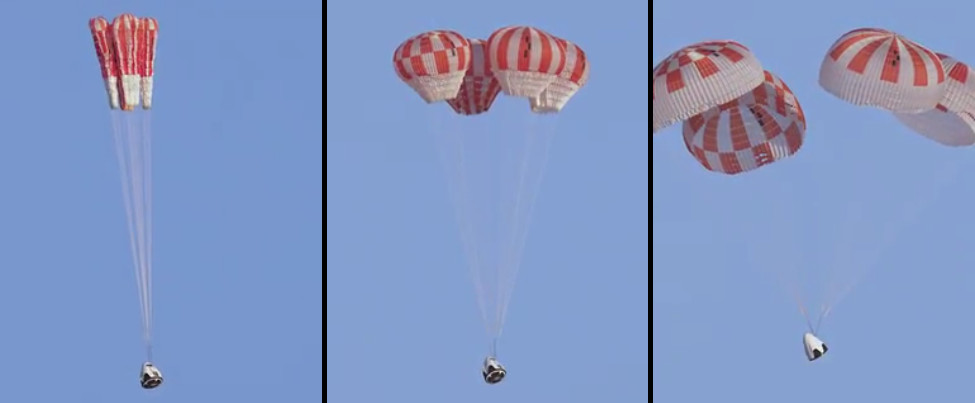
\includegraphics[height=6cm]{images/dragon.jpg}
	\caption{Dragon Reefing System}
	%\vspace{-2ex}
	%\caption*{\textbf{Source:} Original task definition}
	\label{fig:dragon_parachute}
\end{figure}

In the space industry reefing is often achieved by cutting lines inside the parachute. In the \cref{fig:dragon_parachute} above two lines are cut inside the parachute. This is often done by using pyrotechnic line cutters, activated by an electric signal.
\chapter{Requirements Specification}
%\clearpage
\newpage

\section{Requirements Specification} \label{Requirements Specification}
\enlargethispage{2.5cm}
\begin{adjustwidth}{0.23cm}{0cm} \hfuzz=7.0pt \vfuzz=19.0pt
\makebox[\textwidth]{\frame{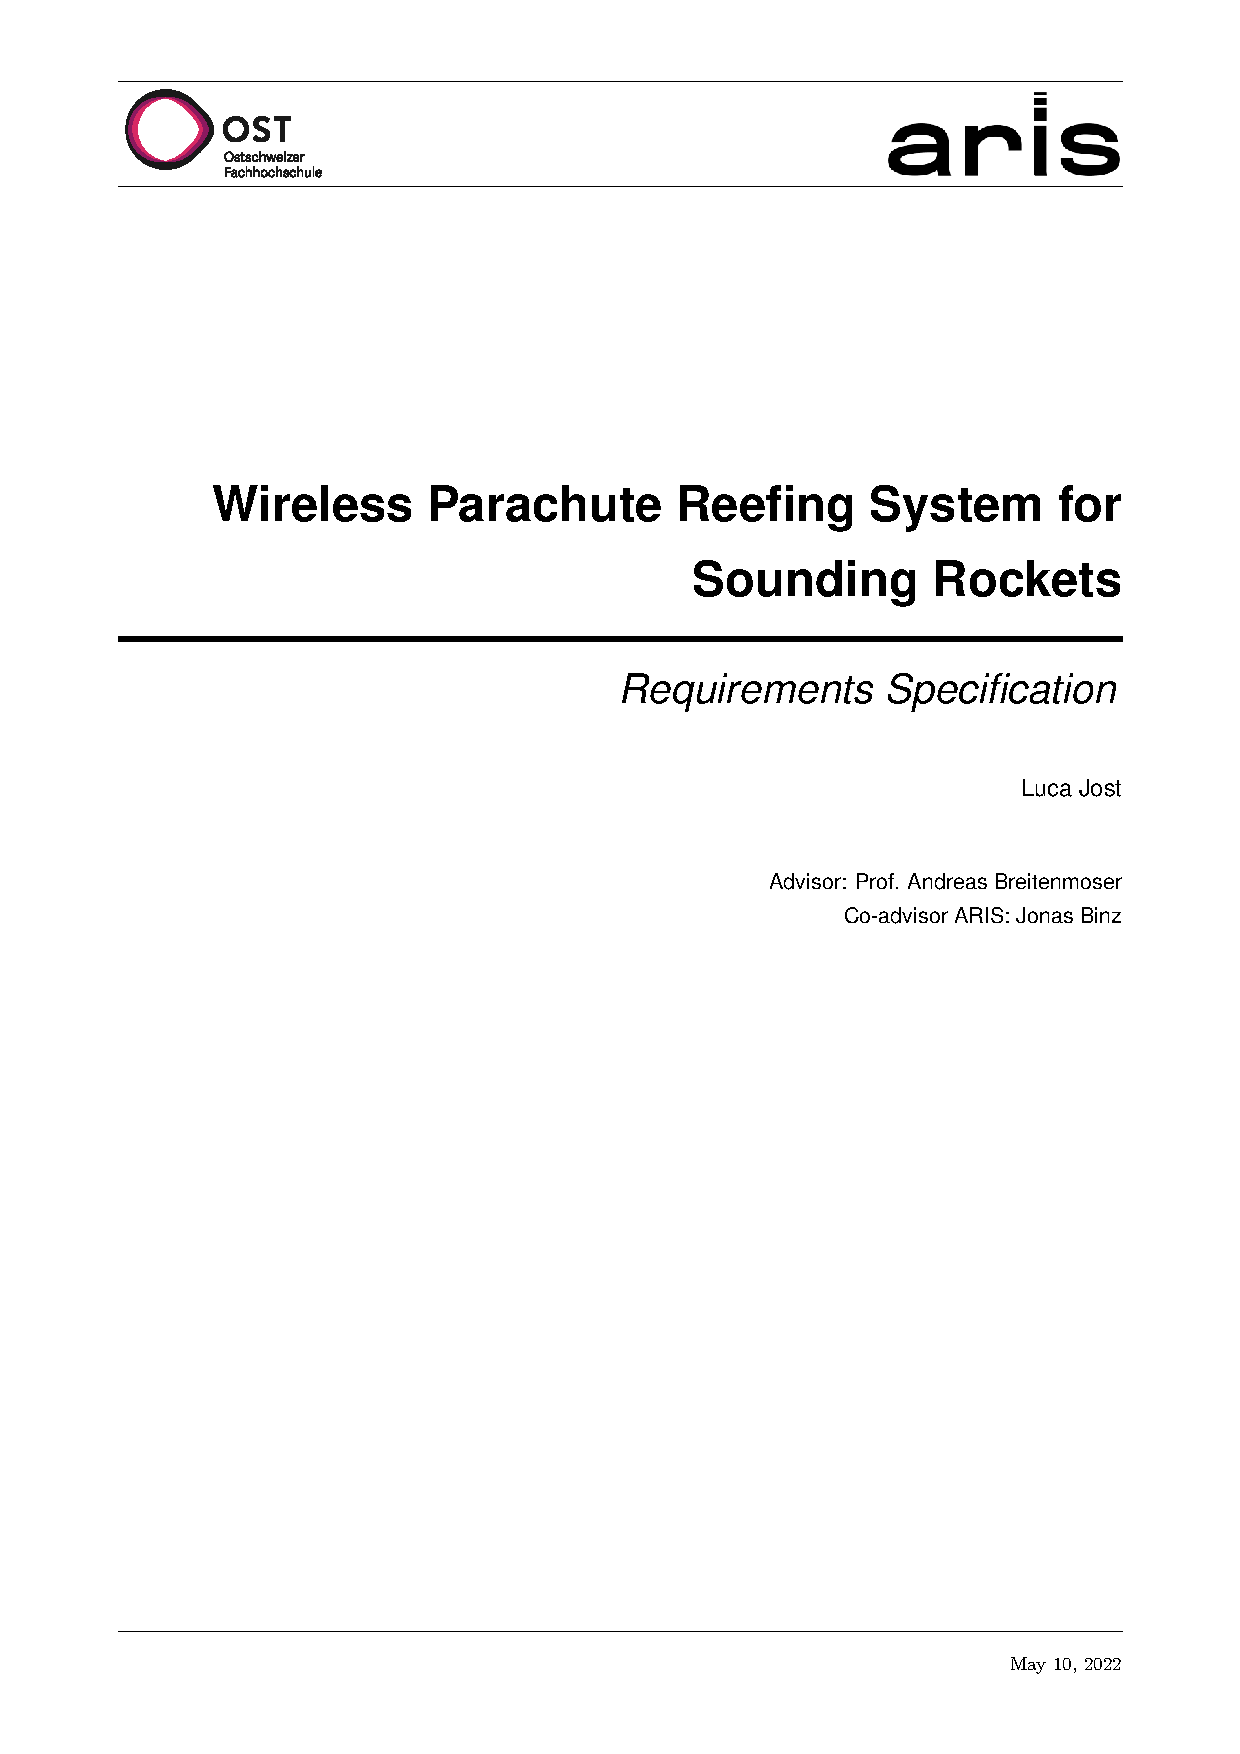
\includegraphics[width=17.3cm, page=1]{appendix/Requirements_Specification}}}
\end{adjustwidth}
\newpage

\begin{adjustwidth}{-0.23cm}{0cm} \hfuzz=7.0pt \vfuzz=19.0pt
\makebox[\textwidth]{\frame{\includegraphics[width=17.3cm, page=2]{appendix/Requirements_Specification}}}
\end{adjustwidth}
\newpage

\begin{adjustwidth}{0.23cm}{0cm} \hfuzz=7.0pt \vfuzz=19.0pt
\makebox[\textwidth]{\frame{\includegraphics[width=17.3cm, page=3]{appendix/Requirements_Specification}}}
\end{adjustwidth}
\newpage

\begin{adjustwidth}{-0.23cm}{0cm} \hfuzz=7.0pt \vfuzz=19.0pt
\makebox[\textwidth]{\frame{\includegraphics[width=17.3cm, page=4]{appendix/Requirements_Specification}}}
\end{adjustwidth}
\newpage

\begin{adjustwidth}{0.23cm}{0cm} \hfuzz=7.0pt \vfuzz=19.0pt
\makebox[\textwidth]{\frame{\includegraphics[width=17.3cm, page=5]{appendix/Requirements_Specification}}}
\end{adjustwidth}
\newpage

\begin{adjustwidth}{-0.23cm}{0cm} \hfuzz=7.0pt \vfuzz=19.0pt
\makebox[\textwidth]{\frame{\includegraphics[width=17.3cm, page=6]{appendix/Requirements_Specification}}}
\end{adjustwidth}
\newpage

\addtolength{\textheight}{\topskip}
\chapter{Preliminaries}

\section{Sounding Rockets}
A sounding rocket is designed to carry scientific payloads and experiments in a suborbital flight profile. The altitude at apogee of sounding rockets varies greatly. As an example, sounding rockets designed by \gls{nasa} can reach altitudes from 50\,km to 1300\,km, while students build high power rockets often only go up to 10\,km. The rocket and, in some cases, only the payload gets recovered by a parachute system. These systems always consist of multiple parachute stages to minimize drift from the launch site.\cite{nasa-rockets}

\begin{figure}[h!]
	\centering
	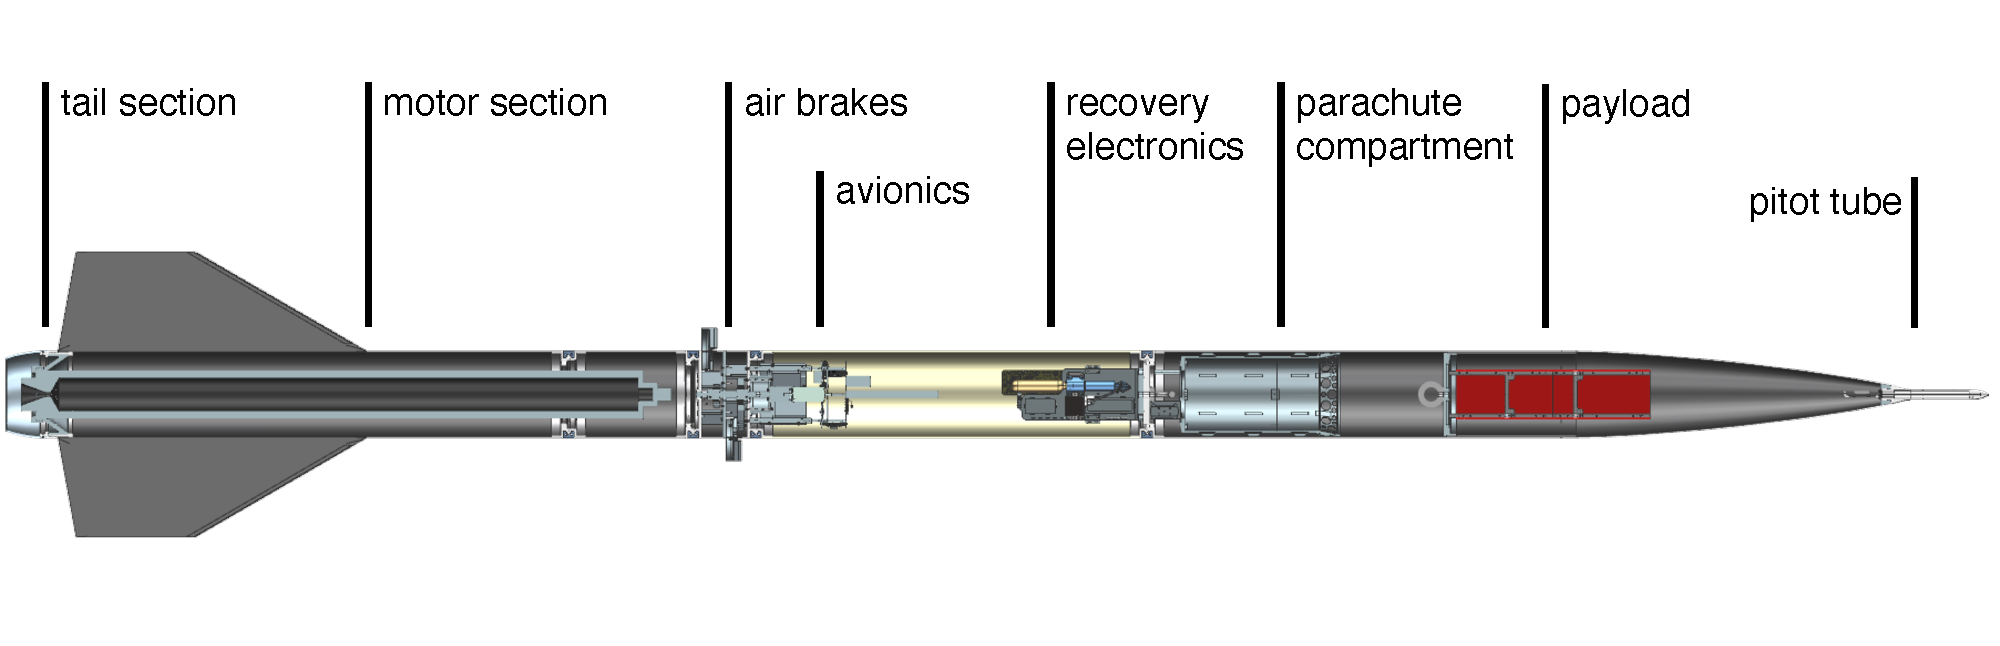
\includegraphics[width=\textwidth]{images/EULER_FSL_CAD}
	\caption{CAD drawing of the rocket EULER from ARIS}
	\caption*{\textbf{Source:} ARIS EULER 2021 EuRoC Report \cite{euler-euroc_report}}
	\label{fig:euler}
\end{figure}

The rocket in Figure \ref{fig:euler} was developed by \acrshort{aris} members for the \acrfull{euroc} in Portugal. It is equipped with an air breaks system to accurately hit a target apogee, an avionics system to transmit telemetry data, and a custom-developed recovery system. The parachute system consists of a drogue and main chute, and a scientific payload can be carried and recovered. The rocket has a dry mass of almost 40\,kg and is 4.2\,m long.  


\newpage

\subsection{Concept of Operation}\label{conops}
Sounding rocket operations are often separated into the phases shown in Figure \ref{fig:operation}.

\begin{figure}[h!]
	\centering
	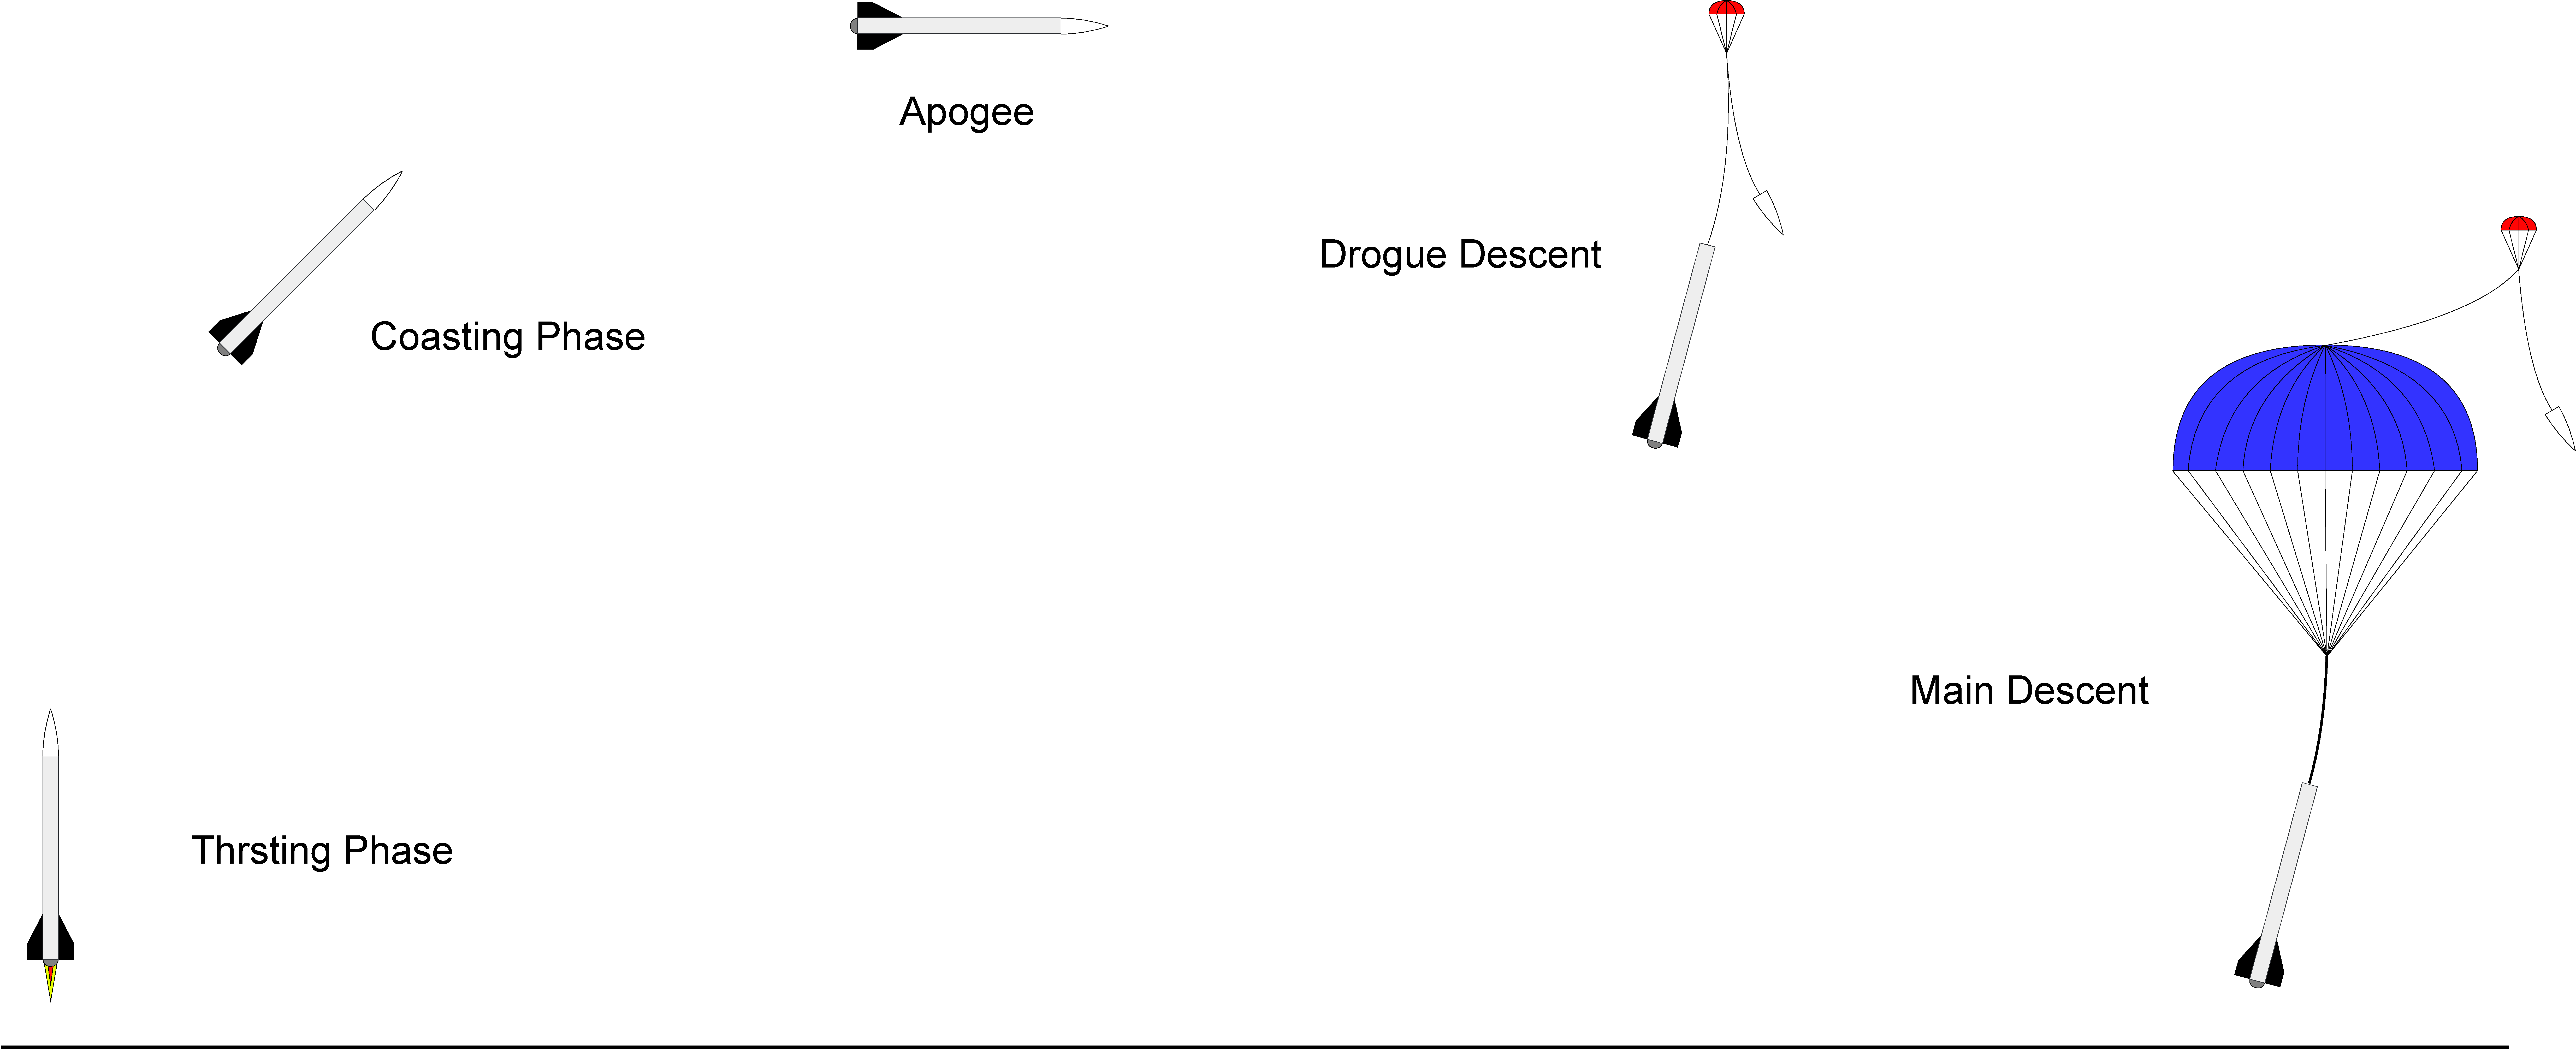
\includegraphics[width=\textwidth]{images/rocket-operation}
	\caption{Illustration of rocket operation}
	\label{fig:operation}
\end{figure}

\subsubsection{Thrusting Phase}
The rocket begins its flight without support from the launch rail and accelerates until the motor burns out. During this phase, accelerations can reach incredibly high numbers, depending on the flight profile. For example, the rockets from the association \acrshort{aris} usually accelerate at around 20\,g but accelerations as high as 100\,g can be experienced. The maximum velocity is reached just at the point of burnout.

\subsubsection{Coasting Phase}
Starting with burnout of the motor, the rocket enters the coast phase. Drag and gravitational forces cause the rocket to decelerate until it reaches apogee. At altitudes above 80\,km, aerodynamic forces are almost nonexistent, leaving the payload exposed to a microgravity environment.

\subsubsection{Drogue Descent}
The drogue parachute sends the rocket into a stable descent to allow a reliable deployment of the main parachute. Drogue parachute deployment causes shock forces to be applied to the rocket structure. For structural reasons, the drogue is often deployed at apogee, where the rocket's velocity is at its lowest point of the flight.

\subsubsection{Main Descent}
In order to minimize the velocity before ground impact, a larger main parachute is deployed close to the ground. The shock loads during the parachute opening are the highest the rocket will experience during its flight. To minimize these forces, a gradual opening of the parachute is preferred.

\newpage

\section{Parachute Reefing}
Parachute reefing permits the gradual opening of the parachute canopy or restricts its full inflation or overinflation. Advantages of parachute reefing include:
\begin{itemize}
		\item Reducing the parachute opening forces. 
		\item Obtain a temporarily high rate of descent. Reefing the parachute to a low drag area permits a more accurate descent from a high altitude. Low-impact velocity is then obtained by disreefing the parachute shortly before ground impact. 
		\item Increase parachute stability by a slight amount of fixed reefing.
\end{itemize}
Two reefing methods are discussed in the following subsections.\cite[Chapter~5.6]{parachute-design}

\subsection{Skirt Reefing}
Skirt reefing is the most commonly used reefing method. 

Reefing rings are located at the connection points of each suspension line inside the canopy skirt. Reefing lines, which are continuous ropes that prevent the canopy from opening, are guided through the reefing rings and several reefing line cutters. Upon firing the cutter at the preset time, it cuts off the reefing line, allowing the canopy to open up or advance to the next stage.

Multiple reefing stages can be added to reduce the forces between each stage.\cite[Chapter~5.6]{parachute-design}

\begin{figure}[h!]
	\centering
	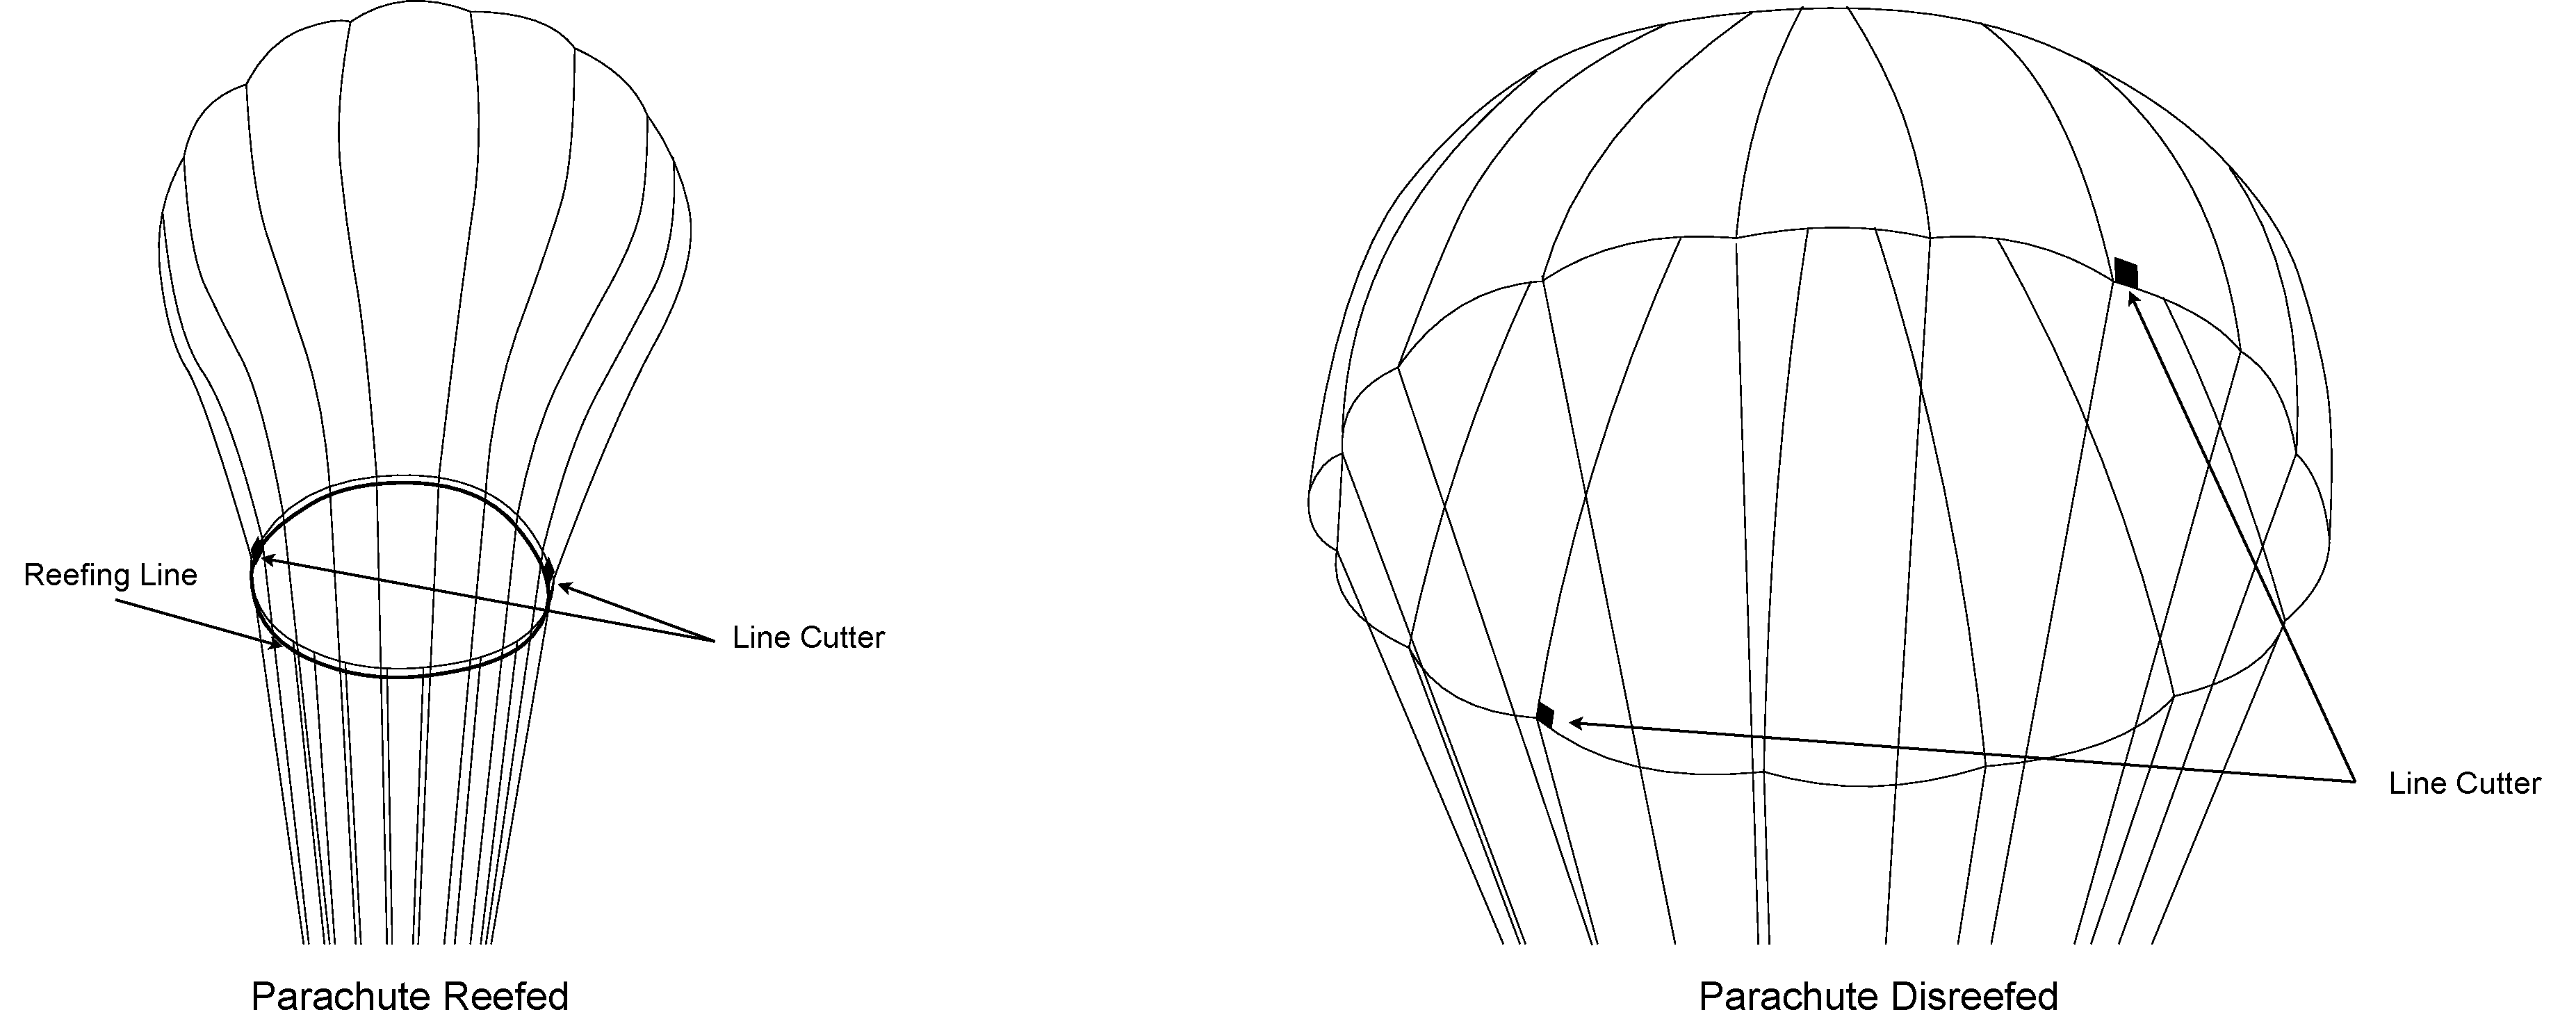
\includegraphics[width=\textwidth]{images/reefing-iilustration}
	\caption{Illustration of skirt reefing system}
	\label{fig:reefing-iilustration}
\end{figure}

\subsection{Continuous Disreefing}
A reefing system in which a pre-selected force-time diagram governs the opening of the parachute canopy is considered the pinnacle of reefing systems. Many attempts have been made to develop such a system. However, none of these attempts resulted in a practical solution.\cite[Chapter~5.6]{parachute-design}

\newpage

\section{Wireless Transmission Methods}

\subsection{Chirp spread spectrum}
\acrfull{css} is a modulation technique used in wireless transmission. It uses its entire allocated bandwidth for broadcast, making it robust to channel noise. The data transmission is based on chirps; a chirp is a sinusoidal signal that linearly increases or decreases in frequency over time. Symbols can be encoded by varying the start frequency as shown in Figure \ref{fig:css}.\cite{css-wiki}

\begin{figure}[h!]
	\centering
	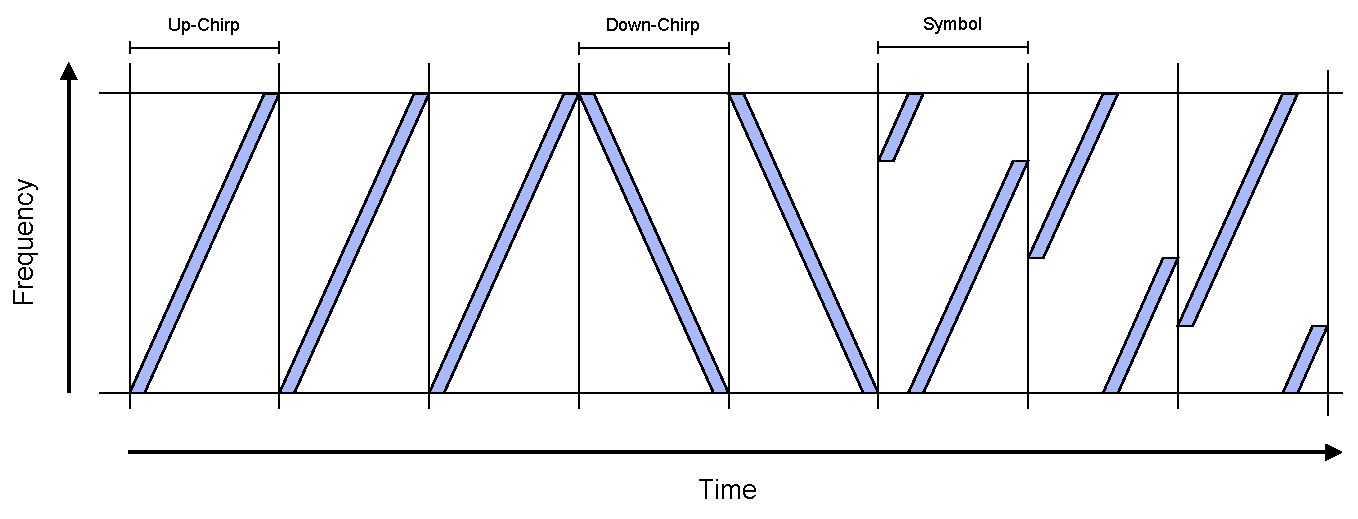
\includegraphics[width=\textwidth]{images/css}
	\caption{\acrshort{css} transmission example}
	\label{fig:css}
\end{figure}

\subsubsection{LoRa}
\acrshort{lora} is a physical proprietary radio modulation technique developed by Cycleo, which Semtech later acquired. \acrfull{css} modulation is used for the transmission. The technology is ideal for applications that transmit small chunks of data with low bit rates. Compared with Wi-Fi, Bluetooth, or ZigBee, data can be transmitted over a longer distance. As a result of these features, \acrshort{lora} is well suited for sensor nodes that operate on a limited power budget.\cite{lora-ttn}

\acrshort{lora} can be operated on the license-free sub-gigahertz bands, such as 915 MHz, 868 MHz, and 433 MHz. It can also work at 2.4 GHz, which achieves higher data rates than sub-gigahertz bands at the expense of range. The frequencies in question are within the ISM bands, reserved internationally for industrial, scientific, and medical uses. \cite{ism-wiki}

The name, \acrshort{lora}, is a reference to the extremely long-range data links that this technology enables. 

\newpage

\subsection{Frequency Hopping Spread Spectrum}
\acrfull{fhss} is a method of transmitting radio signals over rapidly changing carrier frequencies. The frequency band is subdivided into narrow channels. Throughout these channels, signals change their carrier frequencies rapidly in a predetermined order. The transmission requires both the transmitter and receiver to know the hopping pattern. A key benefit of \acrshort{fhss} is that it makes transmissions much more resistant to interference and more difficult to intercept. Allowing more devices on the same frequency band with little or no impact on the link quality.\cite{fhss-wiki}

\begin{figure}[h!]
	\centering
	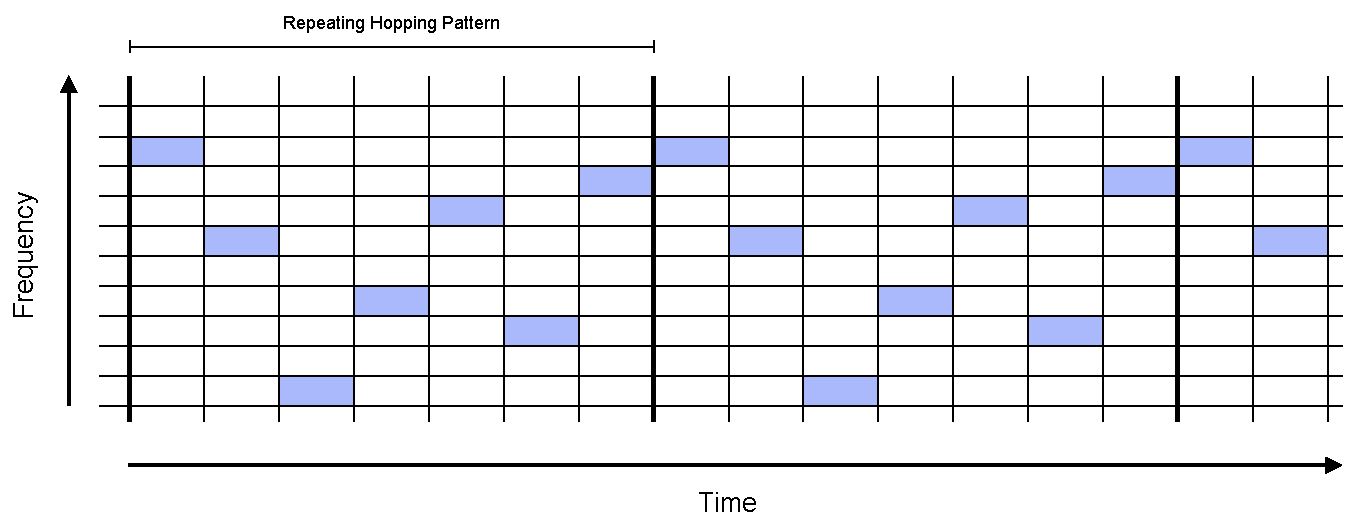
\includegraphics[width=\textwidth]{images/fhss}
	\caption{\acrshort{fhss} transmission example}
	\label{fig:fhss}
\end{figure}

As shown in Figure \ref{fig:fhss}, the frequency is changed with a fixed interval. One of the challenges when developing a \acrshort{fhss} protocol is the synchronization of the transmitter and receiver. The receiver needs to wait for a package to be received. Also, when no data is received, it needs to switch to the subsequent frequency in time. Therefore the time synchronization between the devices is critical. 
\newpage

\section{Kalman Filter}
Kalman filters are used to estimate states based on linear dynamical systems. Using a series of measurements observed over time, including statistical noise and other inaccuracies, the algorithm produces estimates of unknown variables that are usually more accurate than those based solely on a single measurement.

The filter was developed by Rudolf E. Kálmán, after whom the algorithm is named. Although Thorvald Nicolai Thiele and Peter Swerling developed a similar algorithm earlier.\cite{kalman-wiki}

\subsection{Kalman Filter Model}
A Kalman filter is typically built in two phases. A prediction advances the state until the following scheduled observation, while the update step incorporates that observation. It is, however, not necessary for the filter to have two phases. If an observation is not available, the update may be skipped and multiple prediction steps performed. In the same way, if there are several independent observations, multiple updates may be performed as well.\cite{kalman-introduction}

The Kalman Filter model assumes the true state $x_k$ at time ${k}$ from the previous state ${k-1}$. Thus the process model is defined according to
\begin{equation}
    x_{k} = Ax_{k-1} + Bu_{k} + w_{k}
\end{equation}
where
\begin{itemize}
    \item $A$ is the state transition model applied to the previous state $(x-1)$;
    \item $B$ is the control input model applied to the control vector $u_k$;
    \item $w_k$ is the process noise, which is assumed to be a zero mean normal distribution $\mathcal{N} (0, \sigma)$.
\end{itemize}

The measurement model describes the relationship between the state and the measurement at current time $k$. The model takes an observation of the true state  
\begin{equation}
    z_{k} = Cx_{k} + v_{k}
\end{equation}
where
\begin{itemize}
    \item $C$ is the observation model, which maps the true state into the observation state;
    \item $v_k$ is the observation noise, which is assumed to be a zero mean normal distribution $\mathcal{N} (0, \sigma_R)$.
\end{itemize}

\chapter{Conceptual Design}

\section{Line Cutting Methods}

\subsection{Electro-mechanical mechanism}
\subsubsection{Servomotor Actuator}\label{servo-actuator}
A servo motor is a rotary actuator that allows for precise control of the angular position. It consists of a motor coupled to a sensor for position feedback and a drive unit. Hobby-grade servomotors are cheap and available in a variety of sizes.\cite{servo-motor}

For the servomotor actuated concept, the rotary movement of the servo needs to be translated into a linear movement to release the reefing line. The reefing line is attached to both ends of the mechanism. Figure \ref{fig:servo} shows a concept where only one side of the reefing line can be released. The loop in the reefing line is released when the servomotor is actuated, moving the rod down. A concept with two servos to release both loops is feasible, although with the downside of increased weight and size. 

\begin{figure}[h!]
	\centering
	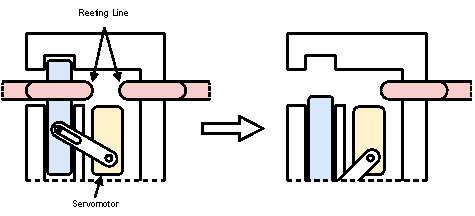
\includegraphics[width=\textwidth]{images/servo}
	\caption{Servomotor release mechanism concept}
	\label{fig:servo}
\end{figure}

\newpage

One of the main issues with this design is the complexity of the mechanical system, and the size and weight constrain. In addition, the loops in the reefing line could entangle with a reefing ring, resulting in a partial opening of the parachute. 

\subsubsection{Linear Solenoid Actuator}
Linear solenoids are electro-mechanical devices that generate a uniform magnetic field when an electric current is applied. They are composed of a coil of wire wrapped around a moveable metal core. The main advantage of solenoid actuators is that the movement is linear; therefore, they can be easily deployed to release a hook.\cite{solenoid-actuator}

The solenoid actuator concept is very similar to the servo actuated release mechanism. As shown in Figure \ref{fig:solenoid}, two solenoid actuators hold on to both ends of the reefing line. The solenoids pull the metal rods down when powered, releasing the reefing line. 

\begin{figure}[h!]
	\centering
	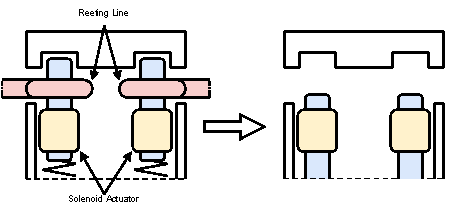
\includegraphics[width=\textwidth]{images/solenoid}
	\caption{Solenoid release mechanism concept (side view, parallel to reefing line)}
	\label{fig:solenoid}
\end{figure}

When solenoids of small size were tried, it was immediately found that they had a meager force. Releasing a reefing line under tension required very large and heavy actuators. Moreover, the same issue described in the servomotor actuated concept also applies to this design. The loops in the reefing line can entangle with reefing rings, preventing the parachute from opening. 

\subsubsection{Continuous Disreefing}
Continous disreefing was briefly considered. In this concept, it was thought of to use a brushless DC motor. The reefing line would be rolled on a spool and then gradually released with the motor. Brushless DC motors can be operated in a constant torque mode, resulting in a very smooth and controlled opening of the parachute canopy.

Some of the significant drawbacks of such a system are complexity, size, and weight.

\newpage

\subsection{Pyrotechnic cutter}
Pyrotechnic cutters were specially designed for this application. They consist of a pyrotechnic charge, a cutting blade, and a piston. On ignition of the pyrotechnic charge, pressure builds up behind the piston, pushing it forward into the reefing line. Severed by the blades, the reefing line is released. Their high reliability and cutting force make them excellent for safety-critical applications. Because of that, pyrotechnic cutters are the industry standard for space and military applications.\cite[Chapter~6.5]{parachute-design}   

\begin{figure}[h!]
	\centering
	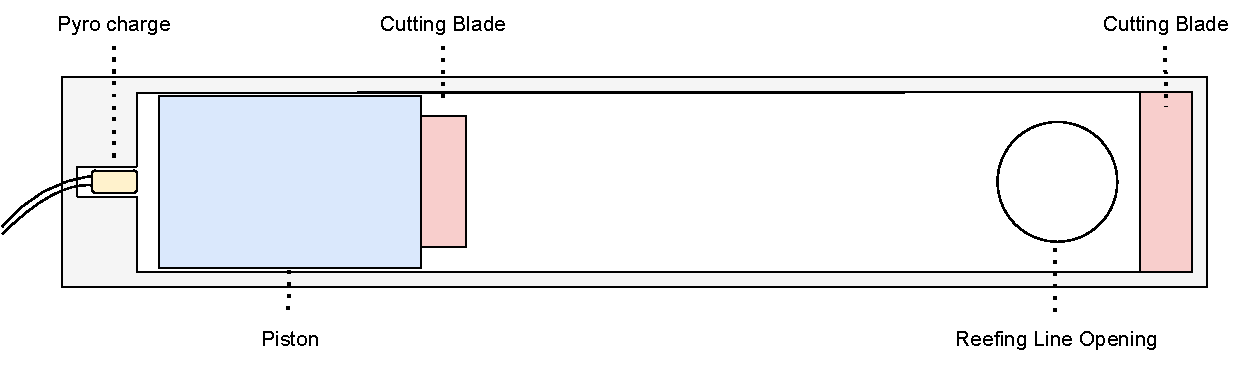
\includegraphics[width=\textwidth]{images/pyro-cutter}
	\caption{Illustration of pyrotechnic line cutter}
	\label{fig:pyro-cutter}
\end{figure}

  Developing a pyrotechnic cutter from scratch was never considered as the author lacks the knowledge of mechanical design. Thus some commercial options were investigated. The Mako Line Cutter from Tinder Rocketry turned out to be a good match for the application. The low weight, high power, and low price are some of the system's advantages. The cutter is advertised to cut paracord, zip ties, and copper wires. Unfortunately, pyrotechnic line cutters are labor- and time-intensive to set up. After every deployment, the igniter, black powder, and a sealing O-ring must be replaced. A turnaround time of fewer than 24 hours is impossible, as epoxy, used to seal the igniter cables, needs to cure overnight.

\begin{figure}[h!]
	\centering
	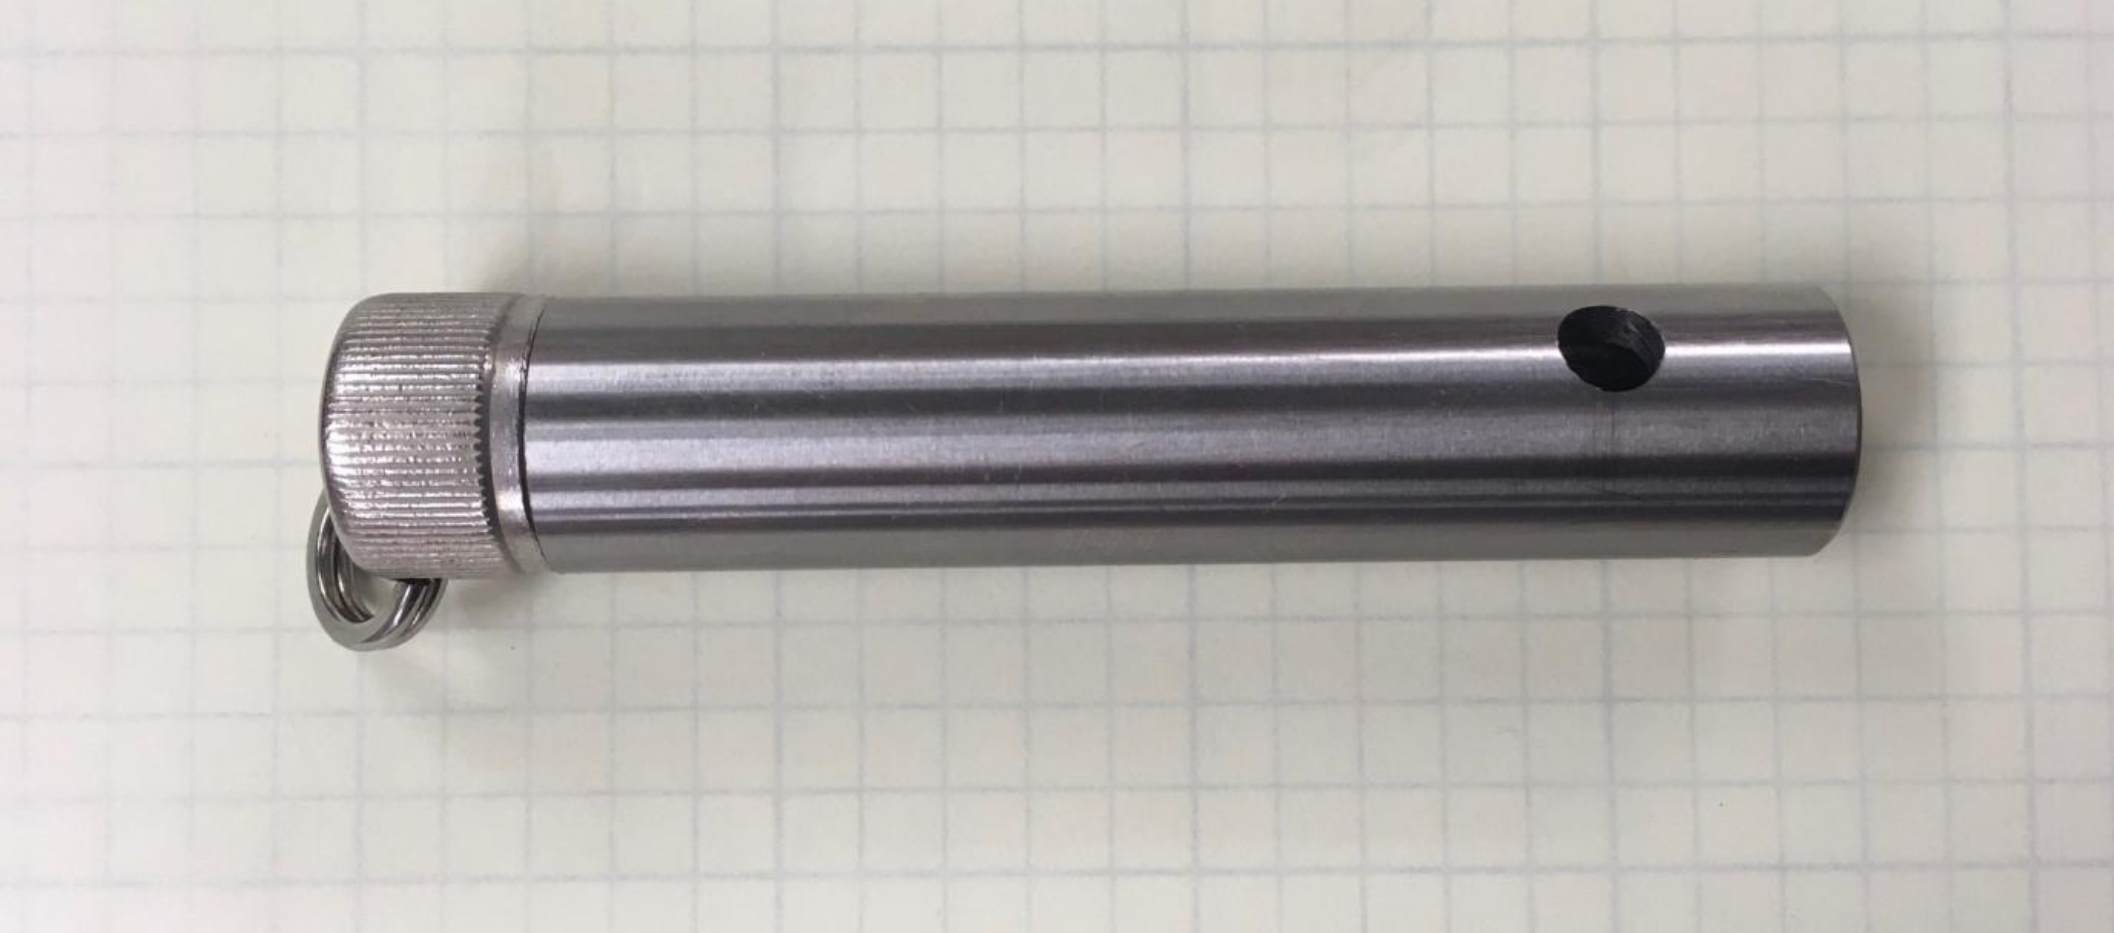
\includegraphics[width=13cm]{images/tinder-rocketry}
	\caption{Make Line Cutter from Tinder Rocketry}
	\caption*{\textbf{Source:} Mako User Instruction Manual  \cite{mako-user-instuction}}
	\label{fig:mako-cutter}
\end{figure}

\newpage


\subsection{Thermal cutter}
During the conceptual design phase, it was identified that the most commonly used parachute lines have a low melting point, making them suitable for thermal separation. Table \ref{tab:thermal-properties} shows the thermal properties of different rope materials.

\begin{table}[h]
    \centering
    \begin{tabular}{ | l | c |}
      \hline
      \textbf{Material}             & \textbf{Melting Point}    \\ \hline
      High Modulus Polyethylene     & 140-150$^\circ$C          \\ \hline
      High Modulus Polyester        & 280-330$^\circ$C          \\ \hline
      Para-aramid                   & 500$^\circ$C $^1$         \\ \hline
      PBO                           & 650$^\circ$C $^1$         \\ \hline
      Polyester                     & 225-240$^\circ$C          \\ \hline
      Polyamide                     & 215-260$^\circ$C          \\ \hline
      Polypropylene                 & 165-175$^\circ$C          \\ \hline
    \end{tabular}
    \caption{\label{tab:thermal-properties}Melting point of commonly used rope materials}
    \caption*{\textbf{Source:} Barry: Technical Properties of Synthetic Fibres \cite{fibers}}
\end{table}
\begin{footnotesize}
        {$1$ Carbonizes before it burns or melts}
\end{footnotesize}

As shown in Table \ref{tab:thermal-properties} all but two of the most commonly used rope materials are suitable for a thermal reefing system. Para-aramid, often branded under the name \textit{Kevlar} is a widespread parachute line material for space missions but is rarely seen in more miniature parachutes. Paracord, designed initially for use as parachute suspension lines, is a lightweight polyamide rope. Due to its strength, elasticity, and comparatively low melting point, it is well suited for a thermal line cutting system.


\subsubsection{Nichrome Wire}\label{nichrome-wire}
Nichrome is widely used in electric heating elements because of its resistance to oxidation, stability at high temperatures, and resistance to the flow of electrons.\cite{nichrome} With a melting point of 1350\,$^{\circ}C$, it can be used to burn through almost all types of ropes. One of the issues with using just a wire is that the rope needs to be in constant contact with the nichrome wire while still being able to move around freely. Therefore, a spring-loaded mechanism was thought of, pushing the nichrome wire against the rope and the case wall. Two posts made out of metal span the nichrome wire across the case. When inserting the reefing line, the springs need to be compressed. One of the drawbacks with this design is that force on the line could damage or rip the nichrome wire. The design was largely inspired by a paper about a release mechanism for CubeSats. \cite{nichrome-cubesats}  

\begin{figure}[h!]
	\centering
	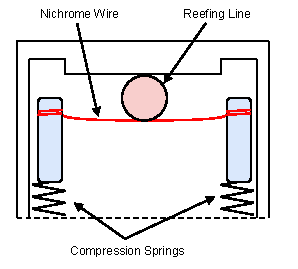
\includegraphics[width=8cm]{images/nichrome-wire}
	\caption{Nichrome wire concept (side view, in line with reefing line)}
	\label{fig:nichrome-wire}
\end{figure}

Initial testing showed that a nichrome wire could burn through a polyamide rope quickly and reliably. Unfortunately, a problem was observed when the reefing line lacked tension. The line would still burn through but melt back together immediately after. The line would stay attached with the nichrome wire out of the way. To combat that, some mechanism is needed to always tension the line. At this point, other thermal options were investigated.

\newpage

\subsubsection{Ceramic Heating Element}
After a long search, commercially available tubular heating elements were discovered. The designed use case for these elements is unknown, but there is some indication that they are being used in electronic cigarettes. The elements are rated to operate at up to 700\,$^\circ$C. The tubular heating element combats all drawbacks from the nichrome wire concept described above \ref{nichrome-wire}. The element's shape allows the rope to move around without transferring force to the heating element.
Additionally, the problem of the wire melting back together is mitigated. However, one of the main drawbacks of the heating element is the high power consumption and the relatively slow temperature rise. Another challenge is that the heating element requires a large voltage and current to be operated.

\begin{figure}[h!]
	\centering
	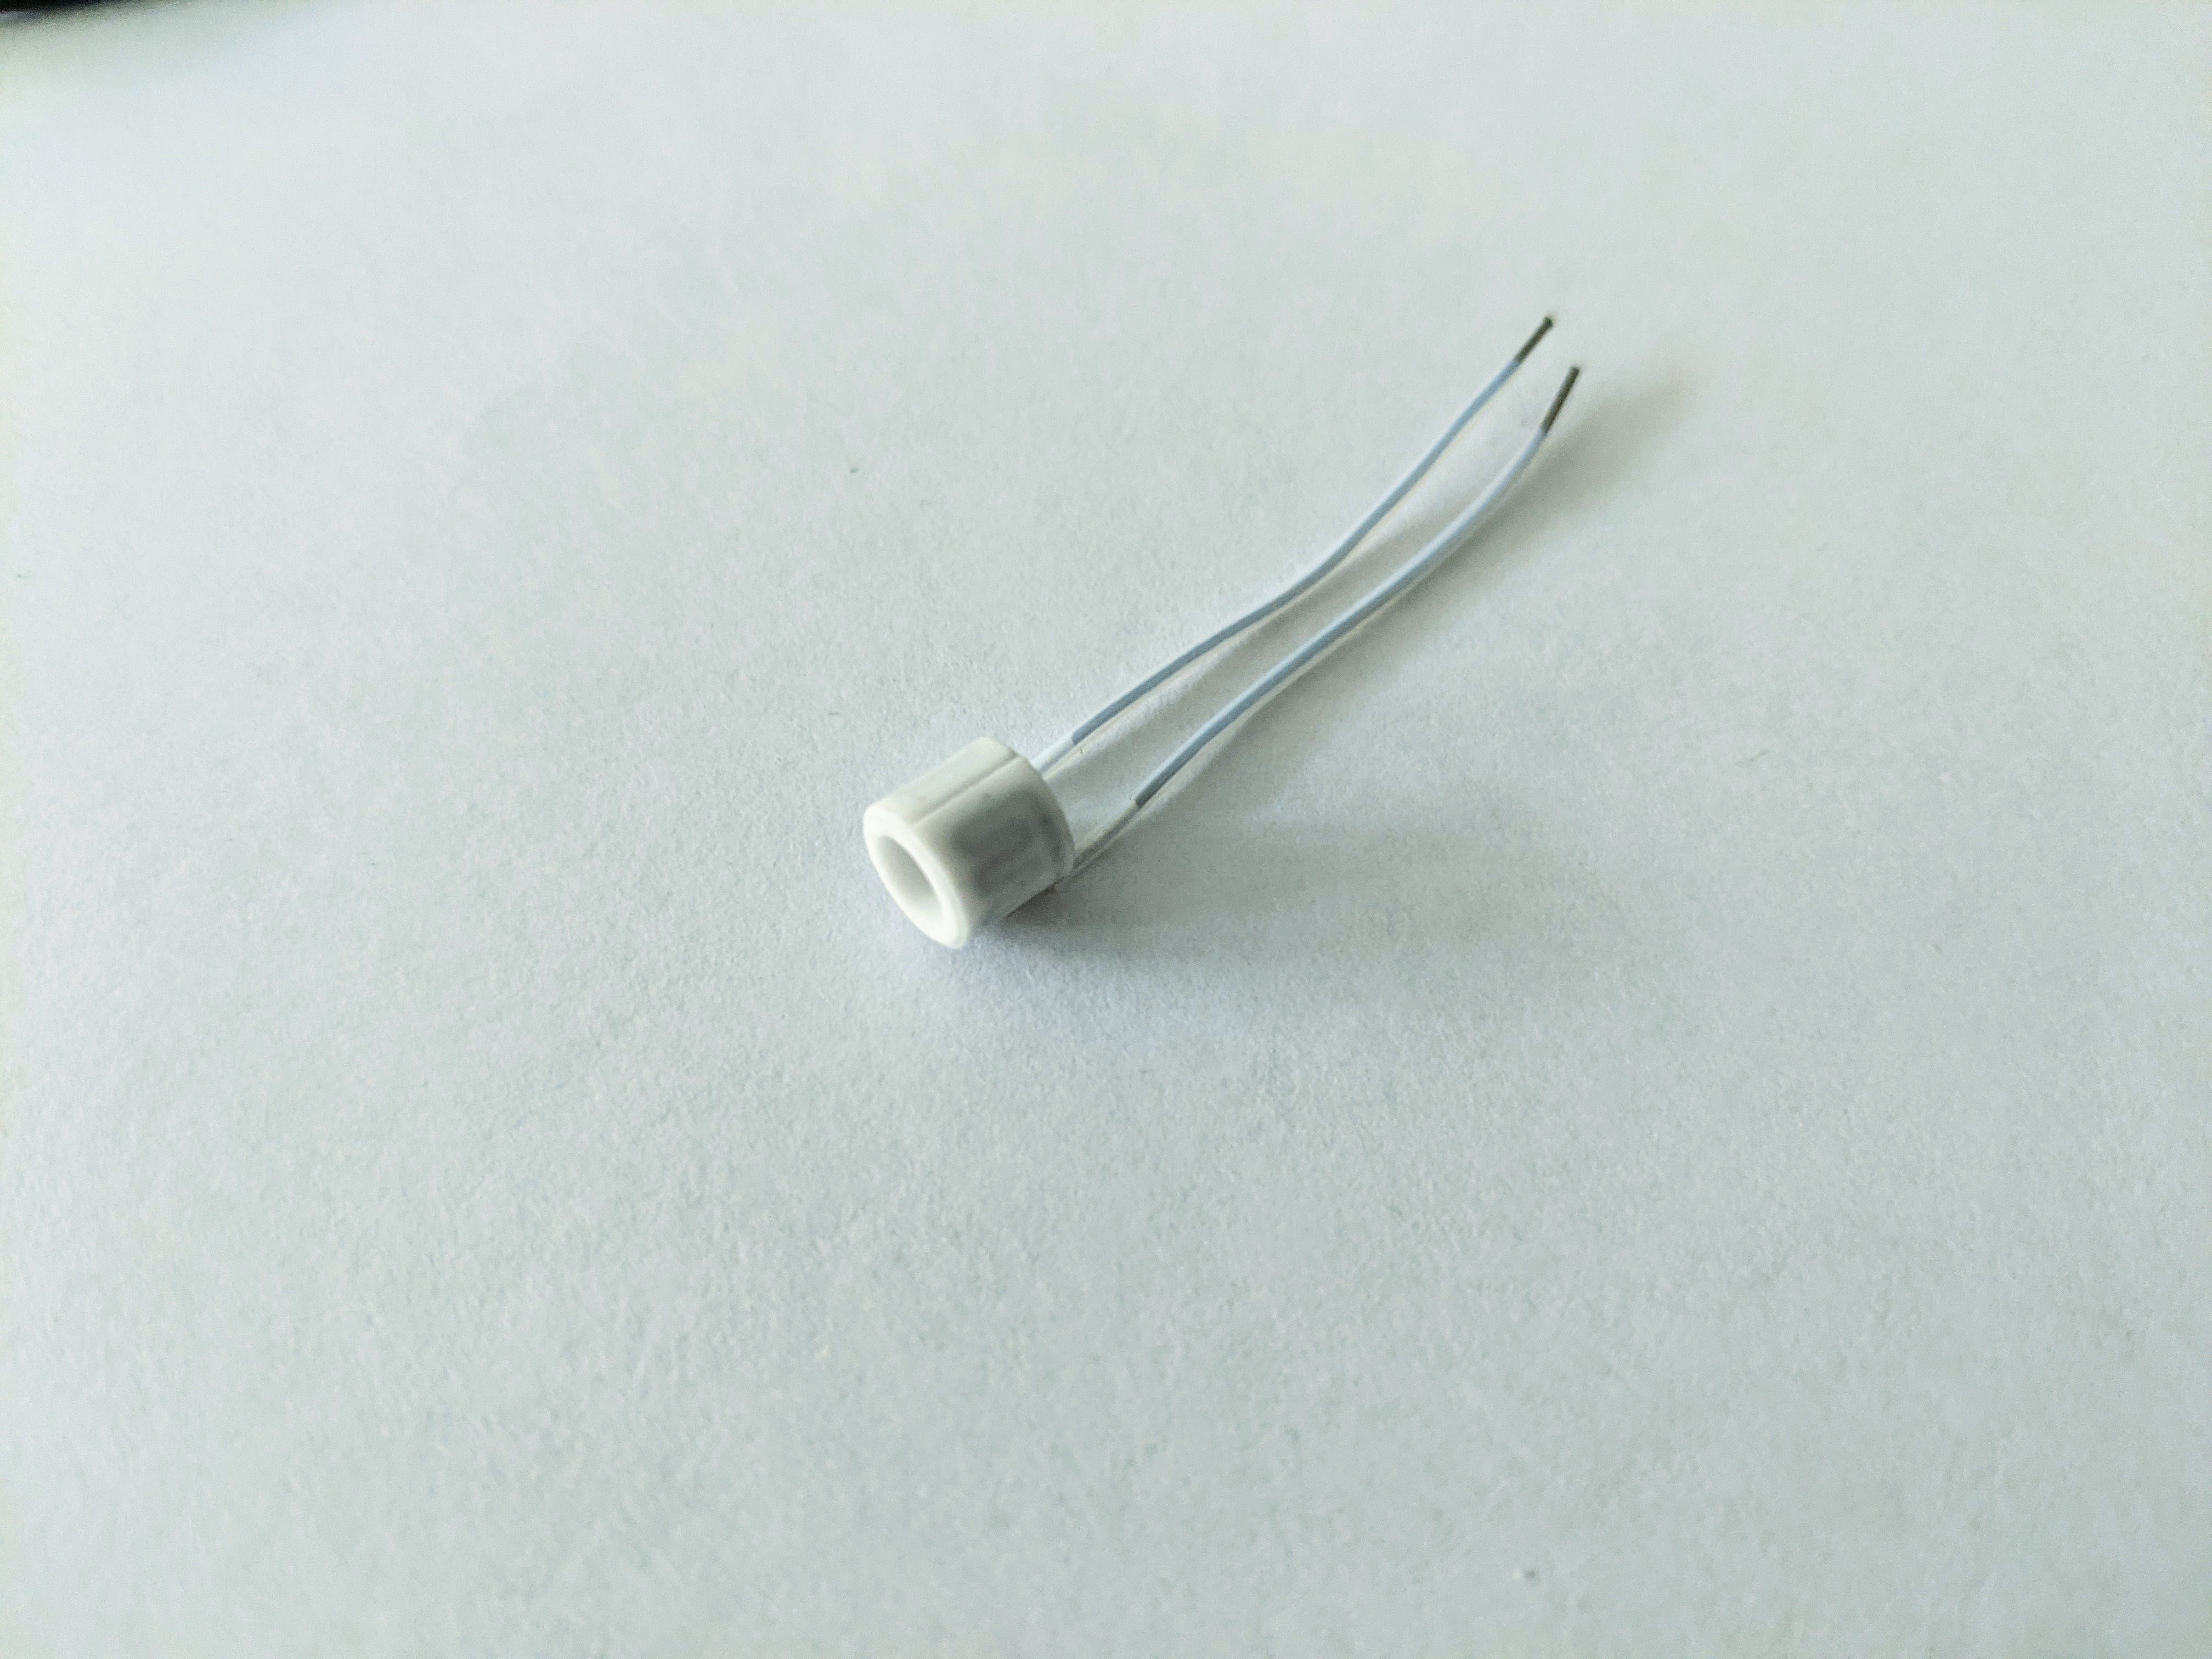
\includegraphics[width=10cm]{images/element}
	\caption{Ceramic Heating element}
	\label{fig:element}
\end{figure}

\newpage

\section{Comparison of Cutting Methods}
A list was created to assess the different cutting methods and decide on a solution. The list was created using the author's limited knowledge, and testing of the different systems and should not be taken as a fact. Especially the reliability is arbitrary and can not be fully assessed before building it. In general, both the electro-mechanical and nichrome wire concepts are medium to low in terms of reliability because the reefing line's force is transferred to the mechanism.  
\begin{table}[h]
    \centering
    \begin{tabular}{ | l | p{2cm} | p{2cm} | p{2cm} | p{1.95cm} |}
      \hline
      \textbf{Method}               & \textbf{Reliability}  & \textbf{Size}  & \textbf{Weight}  & \textbf{Reusable}   \\ \hline
      Servo actuated                & Medium                & Medium         & Medium           & Yes                       \\ \hline
      Linear Solenoid Actuator      & Medium                & Medium         & Medium           & Yes                       \\ \hline
      Continuous Disreefing         & Low                   & Large          & Heavy            & Yes                       \\ \hline
      Pyrotechnic cutter            & Excellent             & Medium         & Medium           & No                        \\ \hline
      Nichrome Wire                 & Medium                & Small          & Light            & Yes                       \\ \hline
      Ceramic Heating Element       & High                  & Small          & Light            & Yes                       \\ \hline
    \end{tabular}
    \caption{\label{tab:cutting-methods}Overview of important line cutter properties}
\end{table}

As shown in Table \ref{tab:cutting-methods}, the pyrotechnic cutter and ceramic heating element are the only two methods that stand out as promising. If the system should be as reliable as possible, pyrotechnic cutters should always be used. However, for this work, reusability was considered more important. Therefore the ceramic heating element cutting method was persuaded.
\chapter{Development}

\section{Hardware Design}
The hardware of the Reefing System was designed using Altium Designer 22. The integrated 3D \acrshort{cad} functionality simplified the overall development and lowered the possibility of errors in the design. The small footprint and consequently extremely dense placement of components required a 6-layer \acrfull{pcb}. The board, with the size of 50\,mm\;x\;35\,mm has been manufactured and assembled by JLCPCB.

\begin{figure}[h!]
	\hspace{-2.2cm}
	\includegraphics[height=11.0cm]{images/render1}
	\caption{Assembled PCB 3D-Render}
	\label{fig:rendering-pcb}
\end{figure}
\newpage

\subsection{Block Diagram}
The hardware block diagram in Figure \ref{fig:hardware-block-diagram} offers an overview of the system architecture. The complete schematic can be found in Appendix \ref{apx:schematic}.  

\medskip
\begin{figure}[h!]
	\centering
	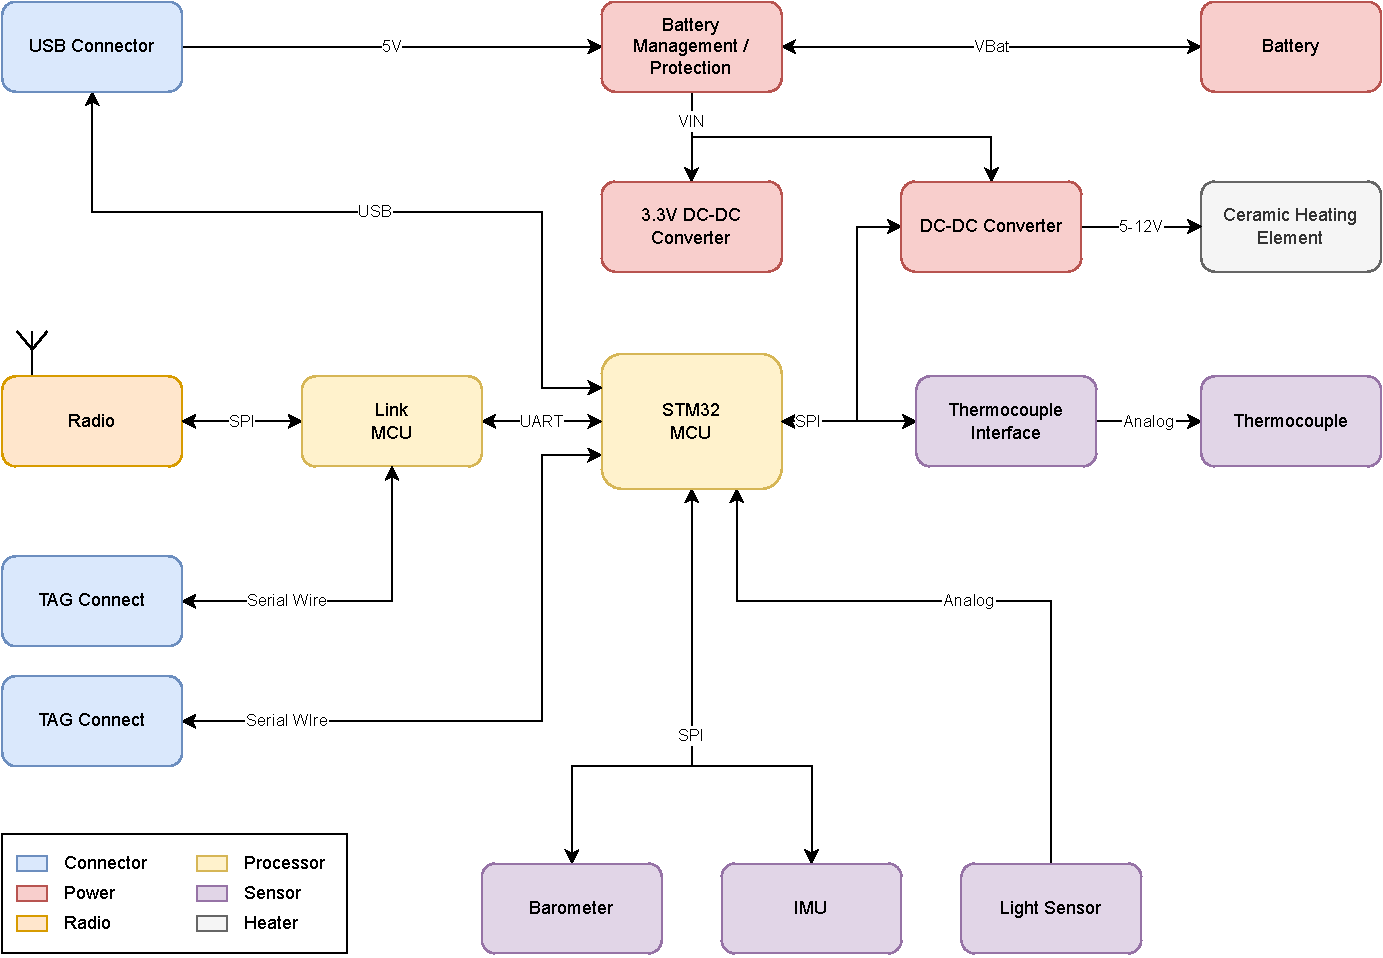
\includegraphics[width=\textwidth]{images/block_diagram}
	\vspace{0.1cm}
	\caption{Hardware Block Diagram}
	\label{fig:hardware-block-diagram}
\end{figure}




\clearpage

\subsection{Microcontroller} \label{microcontroller}
The microcontroller is an essential part of any embedded system. It is the brain of the whole design, processing all incoming and outgoing data.  
\subsubsection{Selection}
Current shortages of chips essentially dictated the selection of a suitable microcontroller. Several factors were carefully considered and key requirements have been set, such as:

\begin{itemize}
		\item System performance: \acrshort{cpu} speed, memory and peripherals
		\item Native \acrshort{usb} 2.0 Interface
		\item Physical package and pin count
		\item Low power draw
		\item Stop mode to preserve battery life
		\item Availability
\end{itemize}

The best suitable \acrshort{mcu} family for the given requirements is the \gls{stm32}L4 ultra-low-power series. Their low power draw and high performance and the native USB 2.0 interface make them ideal for the application. Unfortunately, the availability of the low-power series microprocessors is terrible. Because of that, the decision was taken to go with an older, about as powerful but less efficient, \gls{stm32}F4 microprocessor. In particular, the STM32F411CC was chosen because they were available for assembly by JLCPCB.   

The \acrshort{mcu} selected is based on the high-performance ARM Cortex-M4 32-bit \acrshort{risc} core. Some of its features can be seen in the info graphic \ref{fig:coretex-m4}

\begin{figure}[h!]
	\centering
	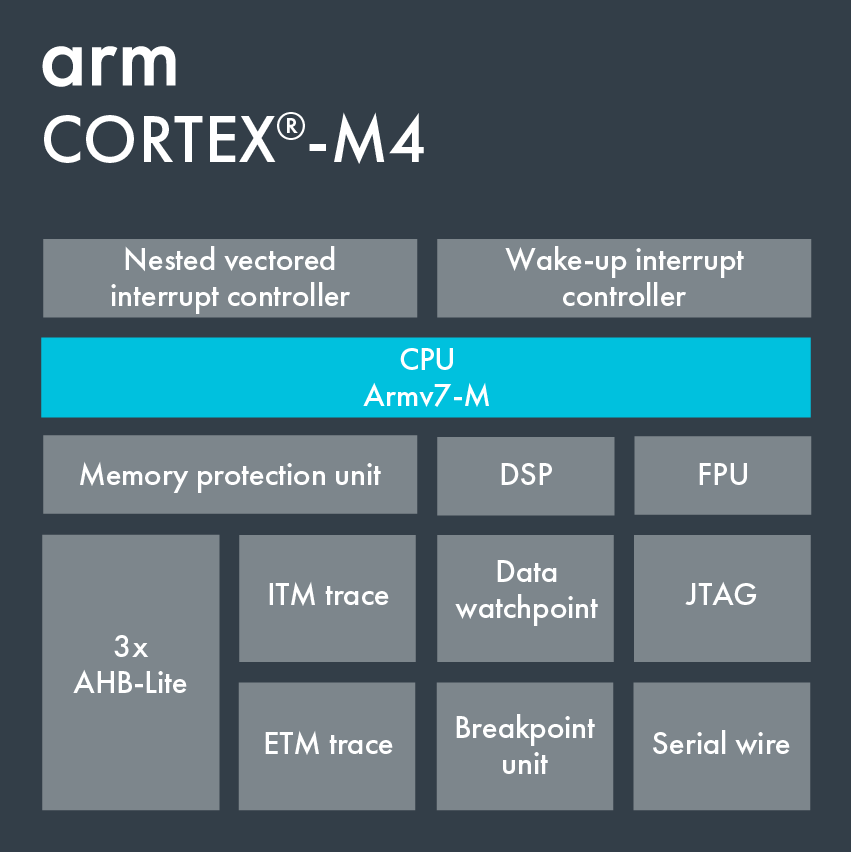
\includegraphics[height=9cm]{images/cortrex-m4}
	\caption{ARM Cortex-M4 Block Diagram}
	\vspace{-1.4ex}
	\caption*{\textbf{Source:} ARM Developer Cortex-M4 Techical Specification \cite{arm-techspecs}}
	\label{fig:coretex-m4}
\end{figure}


\subsubsection{Programming and Debugging}
The \acrshort{mcu} can be programmed over Serial Wire with a suitable programmer (e.g., STMicoroeletronics ST-Link). Through the programmer, debugging is fully supported, allowing fast and efficient software development. 

\subsubsection{Clock Source}
The microprocessor supports clock frequencies up to 100\,MHz. By using an external 8\,MHz crystal oscillator, the main \acrshort{cpu} clock frequency can be adjusted according to the power and processing needs. Another key benefit of an external crystal oscillator is the temperature stability and accuracy of the clock source. However, these factors are not of great relevance for the application.

\subsection{Battery}
The reefing system is permanently attached to a battery. In order to prevent damage to the battery, systems are put in place to protect and monitor it. 

\subsubsection{Battery Selection}
The heating element consumes a lot of current when activated. In order to deliver the currents needed to cut the line, a \acrfull{lipo} battery was selected. In comparison to the more commonly used \acrshort{liion} batteries, \acrshort{lipo} batteries are more power-dense. Meaning they can deliver more current for their size and weight.

The C discharge rating of a battery determines how much current can be pulled from it without overheating. One C is equivalent to a fully charged battery being discharged in one hour. For example, a battery with a rating of 30\,C can dump the whole energy stored in just 2 minutes. The battery selected is a Swaytronic 650\,mAh one cell \acrshort{lipo} battery with a continuous C rating of 35. The battery can be safely discharged at 22.75A, providing enough margin for a successful deployment. 

\begin{figure}[h!]
	\centering
	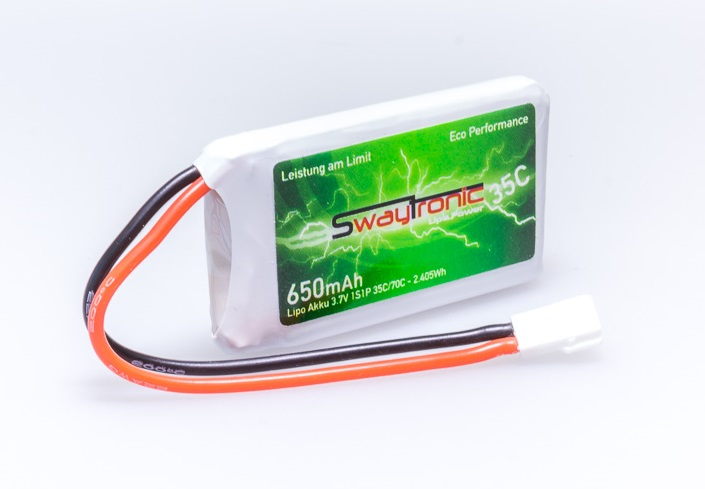
\includegraphics[width=10cm]{images/swaytronic.jpg}
	\caption{Swaytronic 1S 3.7V 650mAh Battery}
	\vspace{-1.4ex}
	\caption*{\textbf{Source:} Swaytronic Webshop \cite{swaytronic}}
	\label{fig:swaytronic}
\end{figure}

\subsubsection{Battery Protection}
In order to protect the battery from under-voltage, over-voltage, and over-current, a battery management chip was selected. Two N-Channel \acrshort{mosfet} operated in a bi-directional switching configuration allow the battery protection \acrshort{ic} to shut off charging or discharging. Whenever the under-voltage threshold is reached, the discharging \acrshort{mosfet} is turned off, allowing the battery to be charged but not further discharged. While charging, as soon as the battery surpasses the minimum allowed voltage, the discharge \acrshort{mosfet} is turned back on. The same goes for an over-voltage event. In that case, charging is disabled, while discharging the battery is possible. 

The under- and over-voltage detection work by measuring the battery voltage directly. The over-current detection, on the other hand, measures the voltage drop across the two \acrshort{mosfet}. For the selected battery protection \acrshort{ic}, the maximum allowed voltage drop across the two \acrshort{mosfet} is 0.15\,V. As soon as that voltage is surpassed, the system gets cut off from the battery. A delay circuit inside the \acrshort{ic} turns the power back on after a short delay. 

\begin{figure}[h!]
	\centering
	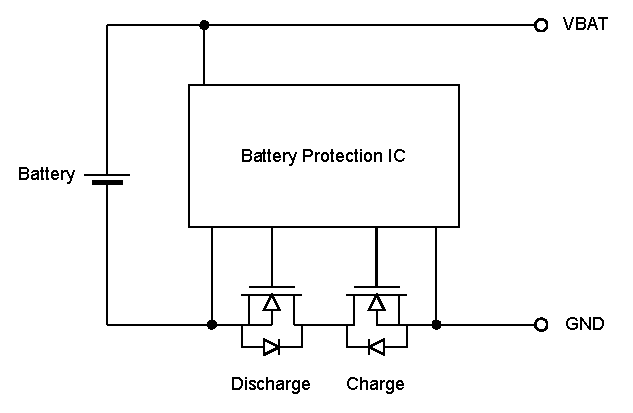
\includegraphics[width=10cm]{images/battery-protection}
	\caption{Simplified Battery Protection}
	\label{fig:battery-protection}
\end{figure}

While cutting a reefing line, the system requires a large current. This current has to be lower than the current limit on the battery protection circuit. Therefore the system was designed to allow a current of at least 15\,A to flow. In order for the system to not trigger over-current events, low internal resistance \acrshort{mosfet} were selected. The Equation \ref{eq:mosfet} shows the maximum allowed internal drain-source resistance of a \acrshort{mosfet} while turned on.

\begin{equation}\label{eq:mosfet}
    R_{DS(ON)} = \frac{U}{2 \times I} = \frac{0.15V}{2 \times 15A} = 5m\Omega
\end{equation}

Initially, some problems with the battery protection circuit were experienced. The battery protection did not switch off whenever the battery voltage reached a critically low voltage, resulting in one of the batteries being deeply discharged. However, only two of the ten boards showed this behavior after much testing. Indication a problem with the assembly, the chip or the \acrshort{mosfet}. No further investigation was conducted.

\subsubsection{Battery Charging}
The battery can be charged through the \acrshort{usb} port on the reefing system. A charging \acrshort{ic} developed by \textit{MicrOne} was used to linearly regulate the 5\,V from the \acrshort{usb} to the battery voltage. The battery is being charged with a constant current until the maximum battery voltage of 4.2\,V is reached. Once the threshold voltage is reached, the charging chip switches to a constant voltage mode. The charging current slowly reaches zero up until the battery is fully charged. Figure \ref{fig:charging-curve} shows an example charge curve of a battery.

\begin{figure}[h!]
	\centering
	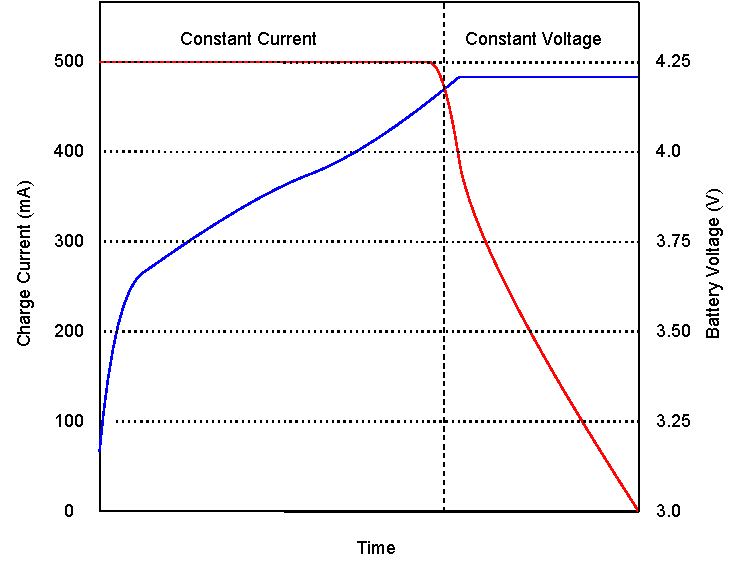
\includegraphics[width=10cm]{images/charge-curve}
	\caption{Example Charge Curve of Lithium Battery}
	\label{fig:charging-curve}
\end{figure}

The charge current can be programmed using a resistor between the \acrshort{ic}s \textit{PROG} pin and ground. Supported are currents of up to 800\,mA. A \acrshort{lipo} battery should not be charged with currents higher than 1\,C. Therefore, a battery with a capacity of 650\,mAh should only be charged with a maximum current of 650\,mA. In order to support a wide range of battery sizes, a jumper was placed on the board that adds a second resistor of the same size in parallel to the first one, doubling the charging current from 300\,mA to 600\,mA. 

\subsubsection{Battery Monitor}
The system can measure the battery voltage using a resistor divider and an analog input on the microcontroller. The voltage divider is built with large resistors, keeping the power dissipation low. A 100\,nF capacitor is used to smooth out the voltage going to the microcontroller. The battery voltage measurement can be reported to the user or used internally for power-saving operations.

\subsubsection{Connector}
Unfortunately, Wire-to-Board connectors rated for the expected currents require a large footprint. For that reason, the battery is soldered directly to the board, providing an extremely low resistance connection with the drawback of not being able to remove the battery quickly.

\newpage

\subsection{Power Management}\label{power-management}

The power management of the system is quite complex. Powering the device from the \acrshort{usb} port, keeping the power draw low while sleeping in addition to the high power draw while cutting, required some clever circuitry. Figure \ref{fig:pm} shows a simplified version of the power management.

\begin{figure}[h!]
	\centering
	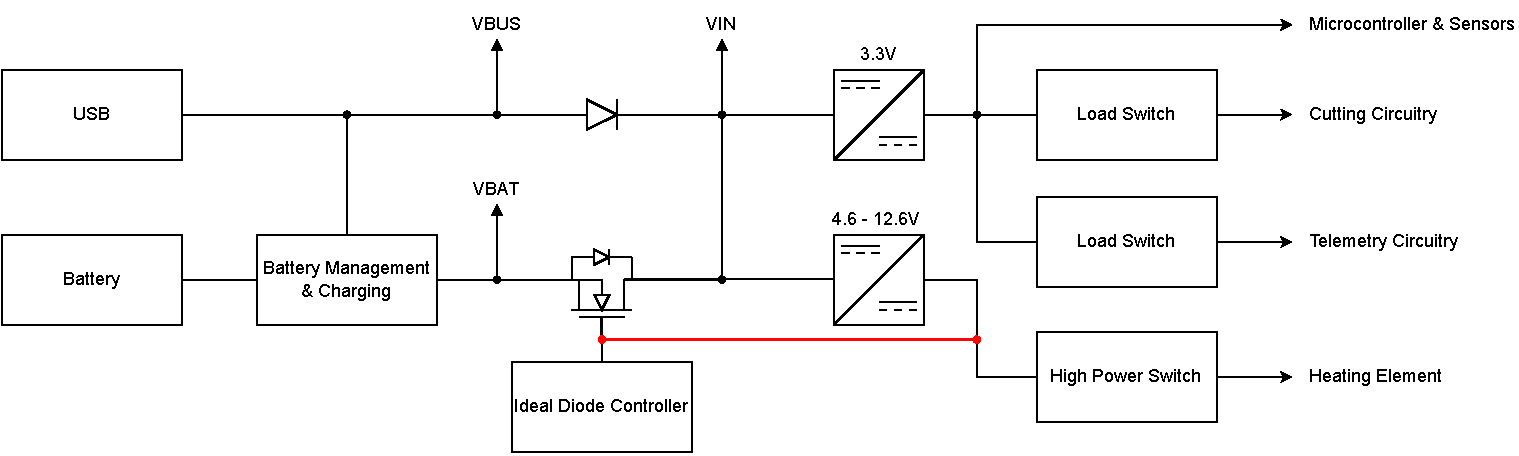
\includegraphics[width=\textwidth]{images/pm}
	\caption{Simplified Power Management of the Reefing System}
	\label{fig:pm}
\end{figure}

\subsubsection{3.3V Power Rails}
In order to keep the power consumption low during sleep modes, multiple power rails were added. The primary power rail is generated from the input voltage using a \acrshort{dcdc} step-down converter. The main power rail, operating at 3.3\,V is connected only to the microcontroller and the sensors operating in low power modes. Two load switches prevent the primary power supply voltage from powering the rest of the system. One of the load switches is intended for all circuitry that powers the cutting mechanism. The second power rail is for the telemetry section. The load switches are operated from the microcontroller, allowing the software to control when each rail is on.

\subsubsection{Heating Element Power Supply}
A \acrshort{dcdc} step-up converter is used to drive the heating element. The TPS61088 is a fully-integrated synchronous boost converter intended for high-power portable applications. The \acrshort{ic} has a wide input voltage range and supports applications with single-cell or two-cell lithium batteries. Texas Instruments rates the \acrshort{ic} to deliver up to 3\,A at 12\,V for a short duration, making it ideal for driving the heating element. The \acrshort{dcdc} converters output voltage can also be adjusted from 4.5\,V to 12.6\,V using a resistor divider. In order to test different heating profiles, a digital potentiometer is used to change the output voltage. The voltage can be adjusted over the full range of the TPS61088 with a step size of around 30\,mV. The digital potentiometer is programmed using \acrshort{spi} and offers 256-taps. 

The \acrshort{dcdc} converter can be powered on and off using the \textit{EN} pin from the TPS61088. Additionally, the heating element can be switched using a power \acrshort{mosfet} allowing for continuous or \acrshort{pwm} operation.

\subsubsection{Ideal Diode and Charging}
While charging, the battery is disconnected from the main power rail, and the current from the \acrshort{usb} is used. This switching was done by using two diodes in parallel. For the battery side, the diode is inside a \acrshort{mosfet}, driven by the ideal diode controller. Resulting in a low voltage drop whenever the system is in flight. The ideal diode controller is turned off as soon as the USB is connected. In that case, the voltage from the USB is always greater than the voltage from the battery, allowing only current to flow from the USB port to the system. 

Unfortunately, the ideal diode controller selected is entirely unavailable for purchase. For that reason, the voltage from the \acrshort{dcdc} step-up converter was used to switch the \acrshort{mosfet}. This fix, which was added after the \acrshort{pcb}s were produced, is shown in Figure \ref{fig:pm} with a red line. With that change, the current consumption in run mode increases but has proven to be working as expected. While sleeping, the \acrshort{dcdc} step-up converter is shut off, allowing current to flow through the diode while preserving battery life. The step-up converter is also shut off immediately when a \acrshort{usb} cable is connected, preventing current from flowing backward into the battery.  

\subsection{Sensors}
\subsubsection{Inertial Measurement Unit}
A \acrfull{imu} was added to the board, intended for liftoff detection and to gather additional data during flight. The LSM6DSR is an ultra-low-power high-performance three-axis linear accelerometer and gyroscope with digital \acrshort{i2c}/\acrshort{spi} serial interface output. The accelerometer inside the sensor has user-selectable scales of ±2\,g up to ±16\,g and can measure with data rates from 1\,Hz up to 6.6\,kHz. The gyroscope has user-selectable scales of ±125\,dps up to ±4000\,dps and provides the same update rates as the accelerometer. The sleep modes provided have an ultra-low power consumption of less than 3\,$\mu$A. Additionally, wake-up on accelerometer action is available, allowing the system to sleep up to the point of rocket liftoff. The sensor is connected through \acrshort{spi} to the microcontroller.

\subsubsection{Barometer}\label{barometer}
A specialized barometric air pressure sensor is used to get altitude information. The sensor has an industry-leading range of 10 to 1200\,mbar allowing for altitude readings of up to around 30\,km above sea level. In addition, the barometer is advertised to have an extremely low power draw of 0.02\,$\mu$A when in standby. Unfortunately, during testing, it was noted that the barometer's current consumption was significantly higher. Contact with the manufacturer was established, but an explanation of that behavior is still pending. The sensor shares the \acrshort{spi} bus with the \acrshort{imu}.

\subsubsection{Thermocouple Interface}
A type-K thermocouple interface was added to monitor the temperature of the heating element. The MAX6675 is designed by Maxim integrated and consists of cold-junction temperature compensation, an analog-digital converter, and a \acrshort{spi} serial interface. The internal \acrshort{adc} with a range of 12\,bit provides a resolution of 0.25\,$^\circ$C and measures up to +1024\,$^\circ$C. Type-K thermocouples provide information about the difference in temperature between two ends of the wires. The cold end, which is the ambient temperature, can fluctuate. The MAX6675 senses and corrects for the changes in the ambient temperature with the cold-junction compensation.

\subsubsection{Light Sensor}
The light sensor is intended to detect the ejection of the parachute. The kind of light sensor used in this application is a phototransistor. In comparison to photodiodes, phototransistors have a much higher gain, allowing for minor light differences to be detected. The collector is connected to the cutting 3.3\,V power rail, reducing current consumption when not in use. The emitter of the sensors is directly connected to a microcontroller \acrshort{adc} pin and a 10\,k$\Omega$ resistor to ground.


\subsection{Telemetry}
The system should be capable of receiving telemetry from the main flight computer of the rocket. For that reason, the telemetry part of the hardware was mostly copied from the existing design of the \gls{cats} flight computer. The \gls{cats} flight computer is the main recovery computer used by \acrshort{aris} in their rockets. 

\begin{figure}[h!]
	\centering
	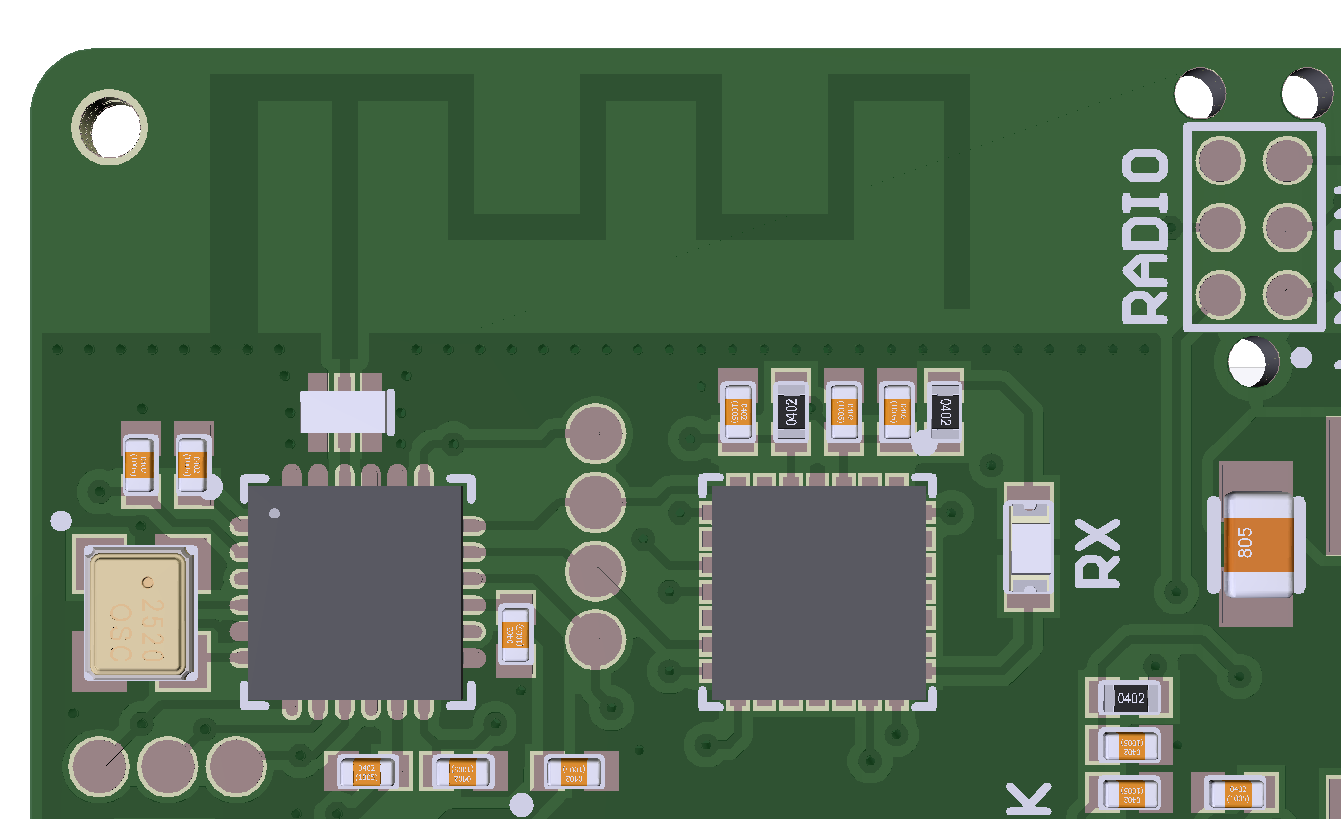
\includegraphics[width=10cm]{images/antenna}
	\caption{Telemetry Section, PCB view}
	\label{fig:antenna}
\end{figure}

\subsubsection{Microcontroller}
The telemetry has a dedicated microcontroller. The task of that microcontroller is to keep the radios synchronized without worrying about other processing tasks. An STM32G071GB was selected for its low price, small footprint, and availability. The \acrshort{mcu} provides no interface for an external crystal oscillator. Therefore the internal one was used. The time stability of the internal oscillator is sufficient to keep time synchronization between the transmitter and receiver.

\subsubsection{Radio}
The radio used for the telemetry link is a Semtech SX1280. It is a \acrshort{lora} 2.4\,GHz \acrshort{rf} transceiver that provides excellent range and low power consumption. An external 52\,MHz crystal oscillator is required, and its frequency gets boosted internally to the carrier frequency. The radio is connected over \acrshort{spi} to the telemetry \acrshort{mcu}. Additionally, two interrupt signals and the busy signal are used for more efficient operation.

\subsubsection{Impedance \& Filter}
The transmission line impedance of the \acrshort{rf} signal line is 50\,$\Omega$. Therefore, close attention was paid to match the \acrshort{pcb} trace to the target impedance by calculating the line thickness and distance to ground. An integrated Altium Designer tool was used for all calculations based on the stack-up of materials and rules added to the transmission lines.  

A \acrshort{ipc} 2.4\,GHz \acrshort{rf} filter was added to the board. A \acrfull{ipc} is a single surface mount component with a filter network built-in. Due to manufacturing and component tolerances, they require considerably less space on the board and often perform better than discrete filters. The main task of the low pass filter is to reduce the harmonics generated by the radio. The selected \acrshort{rf} filter from Johanson Technology matches the transmission line impedance of 50\,$\Omega$.  

\subsubsection{Antenna}
A PCB antenna was added to the board. The design was taken from the Texas Instruments application Note AN043 \cite{ti-antenna}. The antenna chosen has a small footprint and provides good performance. With a reflection of less than -10\,dB over the whole 2.4\,GHz frequency band, the design ensures efficiency of more than 90\,\%. The antenna is linearly polarized and has an omnidirectional radiation pattern. With a matching impedance of 50\,$\Omega$, the antenna requires no additional components on the board. The antenna design can be seen through the solder mask in Figure \ref{fig:antenna}.

\newpage
\section{Mechanical Design \& Line Cutter}

\subsection{Line Cutter}

\subsubsection{Specifications}
The ceramic heating element obtained from Aliexpress has an inner diameter of 4\,mm and an outer diameter of 6.6\,mm. The selected element has an operating voltage of 12\,V. The electrical resistance at room temperature is 8.2\,$\Omega$ and settles at around 18\,$\Omega$ when the maximum temperature of 450\,$^\circ$C is reached. Therefore the power supply needs to deliver a minimum current of 1.5\,A at 12\,V to heat the element quickly. The \acrshort{dcdc} converter, presented in Section \ref{power-management} fulfills this requirement. 

\subsubsection{Insulation}
The heating element needs to be thermally insulated not to burn its surroundings. In order to keep the heat contained, the element is wrapped in multiple layers of fiberglass insulation material. The insulation protects the enclosure from overheating and keeps the heat inside the element, speeding up the separation of the line. In addition, aluminum tape is wrapped around the fiberglass, keeping it in place and reflecting additional heat. The insulating barrier is about 5\,mm thick and keeps the temperatures on the outside below 50\,$^\circ$C after one minute of heating, providing enough margin for the enclosure and surrounding electronics to not be damaged.

\begin{figure}[h!]
	\centering
	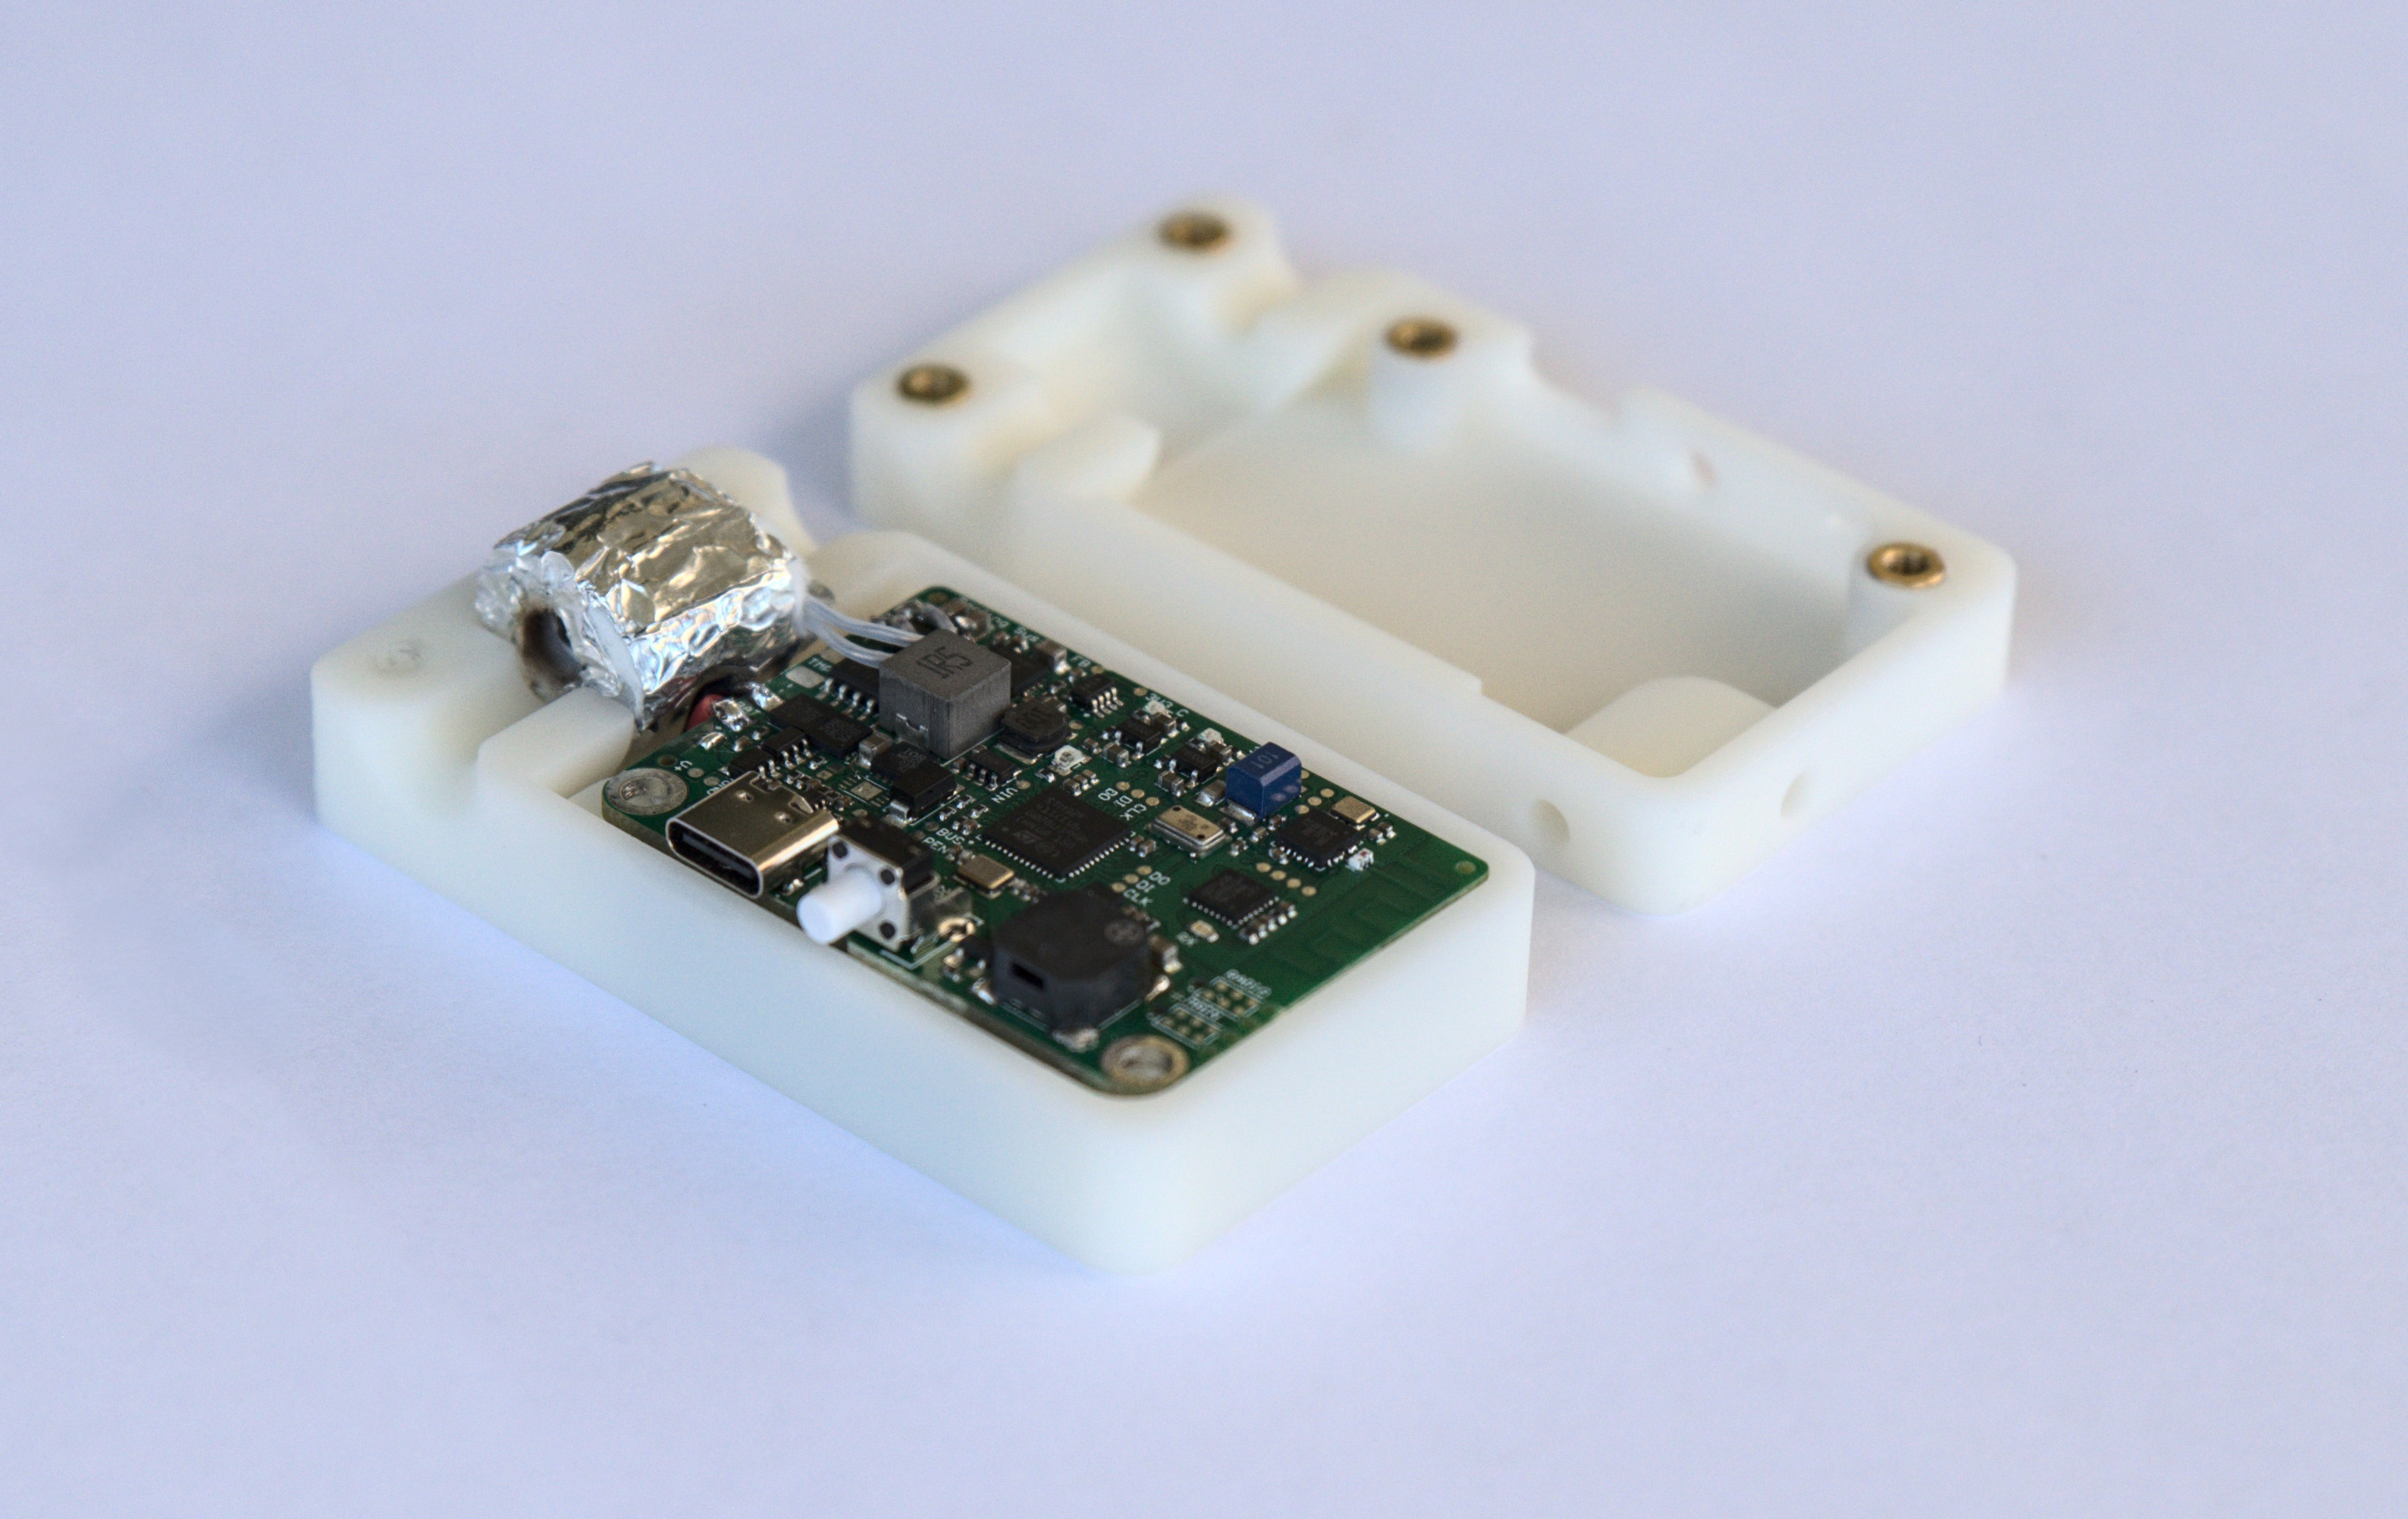
\includegraphics[width=\textwidth]{images/heating-elemet}
	\caption{Open Enclosure with heating element and PCB inside}
	\label{fig:heating-element}
\end{figure}


\newpage

\subsection{Enclosure}
A case for the reefing system was designed using the \acrshort{cad} software SOLIDWORKS 2022. The enclosure is manufactured using a 3D printer. 

\begin{figure}[h!]
	\centering
	\includegraphics[width=8cm]{images/case}
	\caption{Enclosure 3D-Render}
	\label{fig:enclosure}
\end{figure}


\subsubsection{Design}
All parts, the PCB, battery, and heating element were imported into the \acrshort{cad} software in order to design an enclosure around it. The case is built from two halves, the bottom part where the battery and \acrshort{pcb} are mounted and the top part, where holes for the \acrshort{usb} connector and button are placed. A set of M3 screws are used to assemble the enclosure. Threaded inserts, added after printing, make it possible to open and close the case repeatedly. The heating element is clamped together, and channels guide the reefing line to the heating element. 

\subsubsection{Manufacturing}
Initial prototypes were printed using \acrshort{pla} plastic filament on a \acrshort{fdm} printer. \acrfull{fdm} is a method of additive manufacturing where layers of materials are fused together. The material is melted and then extruded in a pattern next to or on previous extrusions, creating an object layer by layer. The main advantage of this manufacturing process is the fast and cheap process. 

The final design is manufactured using LEDO 6060 plastic. Compared to the \acrshort{pla} plastic filament, it provides better dimensional stability and good temperature resistance. The parts are manufactured using a \acrfull{sla} printer. Other than the \acrshort{fdm} process, the printers use a light source to cure liquid resin into hardened plastic. JLCPCB manufactured the enclosure. They print the design on industrial-grade machines resulting in excellent surface finish and accuracy.

\newpage

%% Section Firmware %%
\section{Firmware}
The firmware is written in C and is based on the STMicroelectronics \acrshort{hal} libraries. As an \acrshort{ide}, CLion together with CubeMX is used. This modern environment ensures rapid and efficient development.\newline
FreeRTOS is the real-time operating system of choice. It guarantees a reliable operation and handles multi-task operations on single-core systems.

\subsection{Operation}\label{operation}

The state event diagram in Figure \ref{fig:fsm} offers an overview of the behavior of the system.

\begin{figure}[h!]
	\centering
	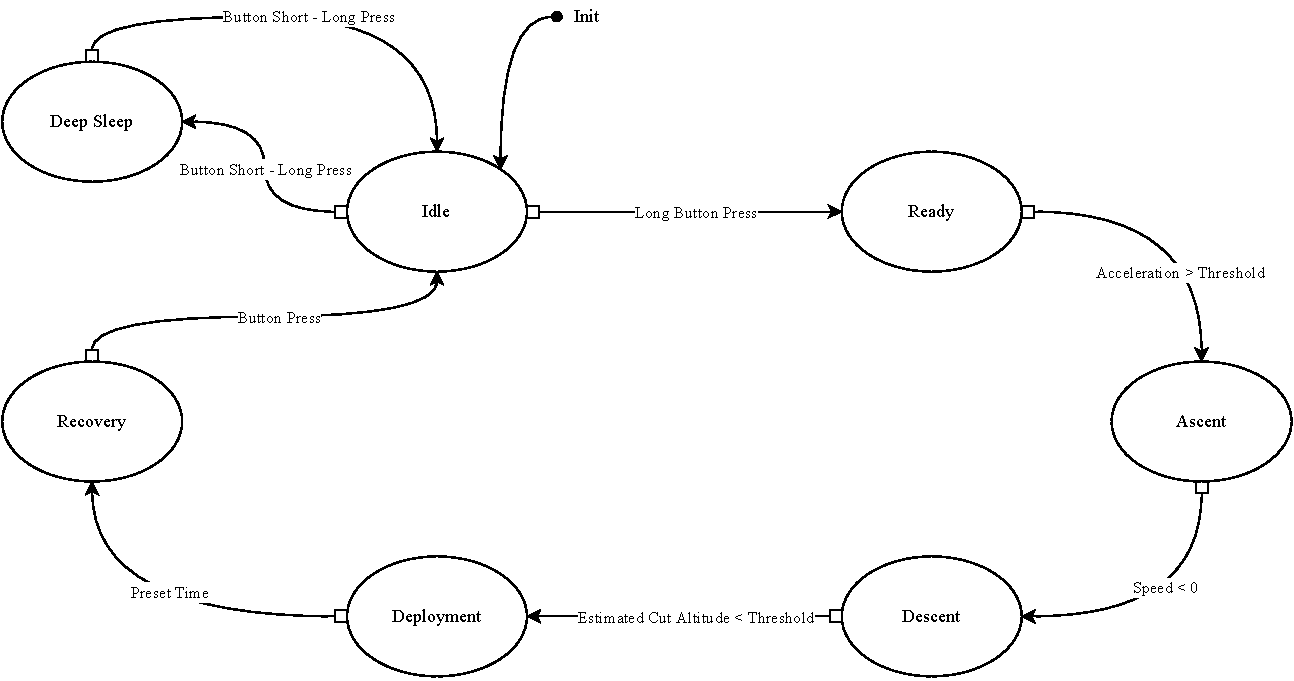
\includegraphics[width=\textwidth]{images/fsm}
	\caption{Finite State Machine}
	\label{fig:fsm}
\end{figure}

\subsubsection{Deep Sleep}
During deep sleep, the microcontroller is put into stop mode, all auxiliary power rails are turned off, and the sensors are put into sleep mode. During deep sleep, the power consumption is minimized to preserve battery life. In addition, all interrupts except for the button pin are turned off. Therefore the system can only be woken up by user input.  

\subsubsection{Idle}
When woken up from deep sleep, the system goes into idle mode. The user can configure the device through the USB port or check the battery life during this state. If the device is inactive for over a minute, it will automatically return to deep sleep. Before liftoff, with user input, the device can be put into ready mode.

\subsubsection{Ready}
In the ready state, both the barometer and accelerometer are constantly readout. The barometric air pressure data is used to calculate the altitude and passes through a Kalman filter. After 30 seconds, the microcontroller puts the accelerometer in wake-up mode and goes to stop mode—preserving battery life before the rocket's liftoff. An acceleration event triggers an interrupt and puts the microcontroller back into run mode. If the acceleration is greater than a user set threshold for over 100\,ms, the rocket's liftoff is detected. User input during the ready state can transition the finite state machine back into idle mode. 

\subsubsection{Ascent}
After liftoff is detected, the rocket ascends to apogee. The barometer is read out and passed through the state estimation during this phase. The estimated vertical velocity is used to detect the highest point in the flight. At that point, the vertical velocity hits zero and becomes negative. As soon as the velocity sign changes, the apogee is reached, and the finite state machine advances to the descent phase.

For short-duration flights, the heating element is getting preheated as soon as liftoff is detected. The temperature only slowly rises and does not damage the reefing line by applying a lower voltage to the element. Preheating is only recommended on very short flights if there is not enough time for the element to heat up between apogee and the main altitude. 

\subsubsection{Descent}
During the descent phase, the velocity and altitude are read out continuously. With the data obtained, the deployment altitude is calculated and initiates the separation as soon as the following criteria applies:
\begin{equation}
    h_{deploy} < (h + v \times t_{burn}) 
\end{equation}
where
\begin{itemize}
    \item $h_{deploy}$ is the user set deployment altitude in m;
    \item $h$ is the current altitude in m;
    \item $v$ is the current velocity in m/s;
    \item $t_{burn}$ is the estimated burn duration in s;
\end{itemize}

\subsubsection{Recovery}
After separating the lines, the system goes into recovery mode. The reefing system continuously beeps, making the recovery operation of the rocket easier. The device can be disabled with user input, returning to the idle state.

\newpage

\subsection{RTOS}
The system is running on FreeRTOS, an open-source, free-to-use \acrlong{rtos} developed by Real Time Engineers Ltd. The operating system runs with a tick rate of 1000\,Hz while most tasks operate at 100\,Hz. Seven tasks are running simultaneously while the system is in flight. The sensor readouts, state estimation, and finite state machine operate at 100\ Hz. Event-based tasks, like the buzzer, execute only once whenever requested. The health monitor, telemetry, and heater operate at a fixed frequency of 10\,Hz.

The \acrshort{rtos} is operated with preemption enabled, allowing task switching. All tasks are running with the same priority, preventing deadlocks but with the downside of slowing down the system if a task is blocked.   

\subsection{Sleep Mode}
As already described in Section \ref{operation} the microcontroller can be put in to stop mode to preserve battery life. The microcontroller is in the deepest possible sleep mode with memory retention in this operating state. All clock sources are turned off, and the low power regulator is used. From the datasheet, in this configuration, the current consumption of the \acrshort{mcu} is reduced to around 38\,$\mu$A. Outside the chip, all power rails, except for the main 3.3\,V supply, are turned off, and all sensors are put in standby mode. The only wake-up source in sleep mode are external interrupts. Only the button can wake the system up in the deep sleep state. While during the ready state, both the button and the accelerometer interrupt can return the \acrshort{mcu} from stop mode.  

According to some calculations ahead of time, the power consumption of the whole system in deep sleep mode should not exceed 100\,$\mu$A. But unfortunately, the measured current is a lot higher. As explained in Section \ref{barometer}, the main cooperate for the high consumption is the barometer. All current measurements were done using the NORDIC Semiconductors Power Profiler Kit II. The 200\,nA to 1\,A range made it possible to monitor the power consumption accurately.  

\begin{figure}[h!]
	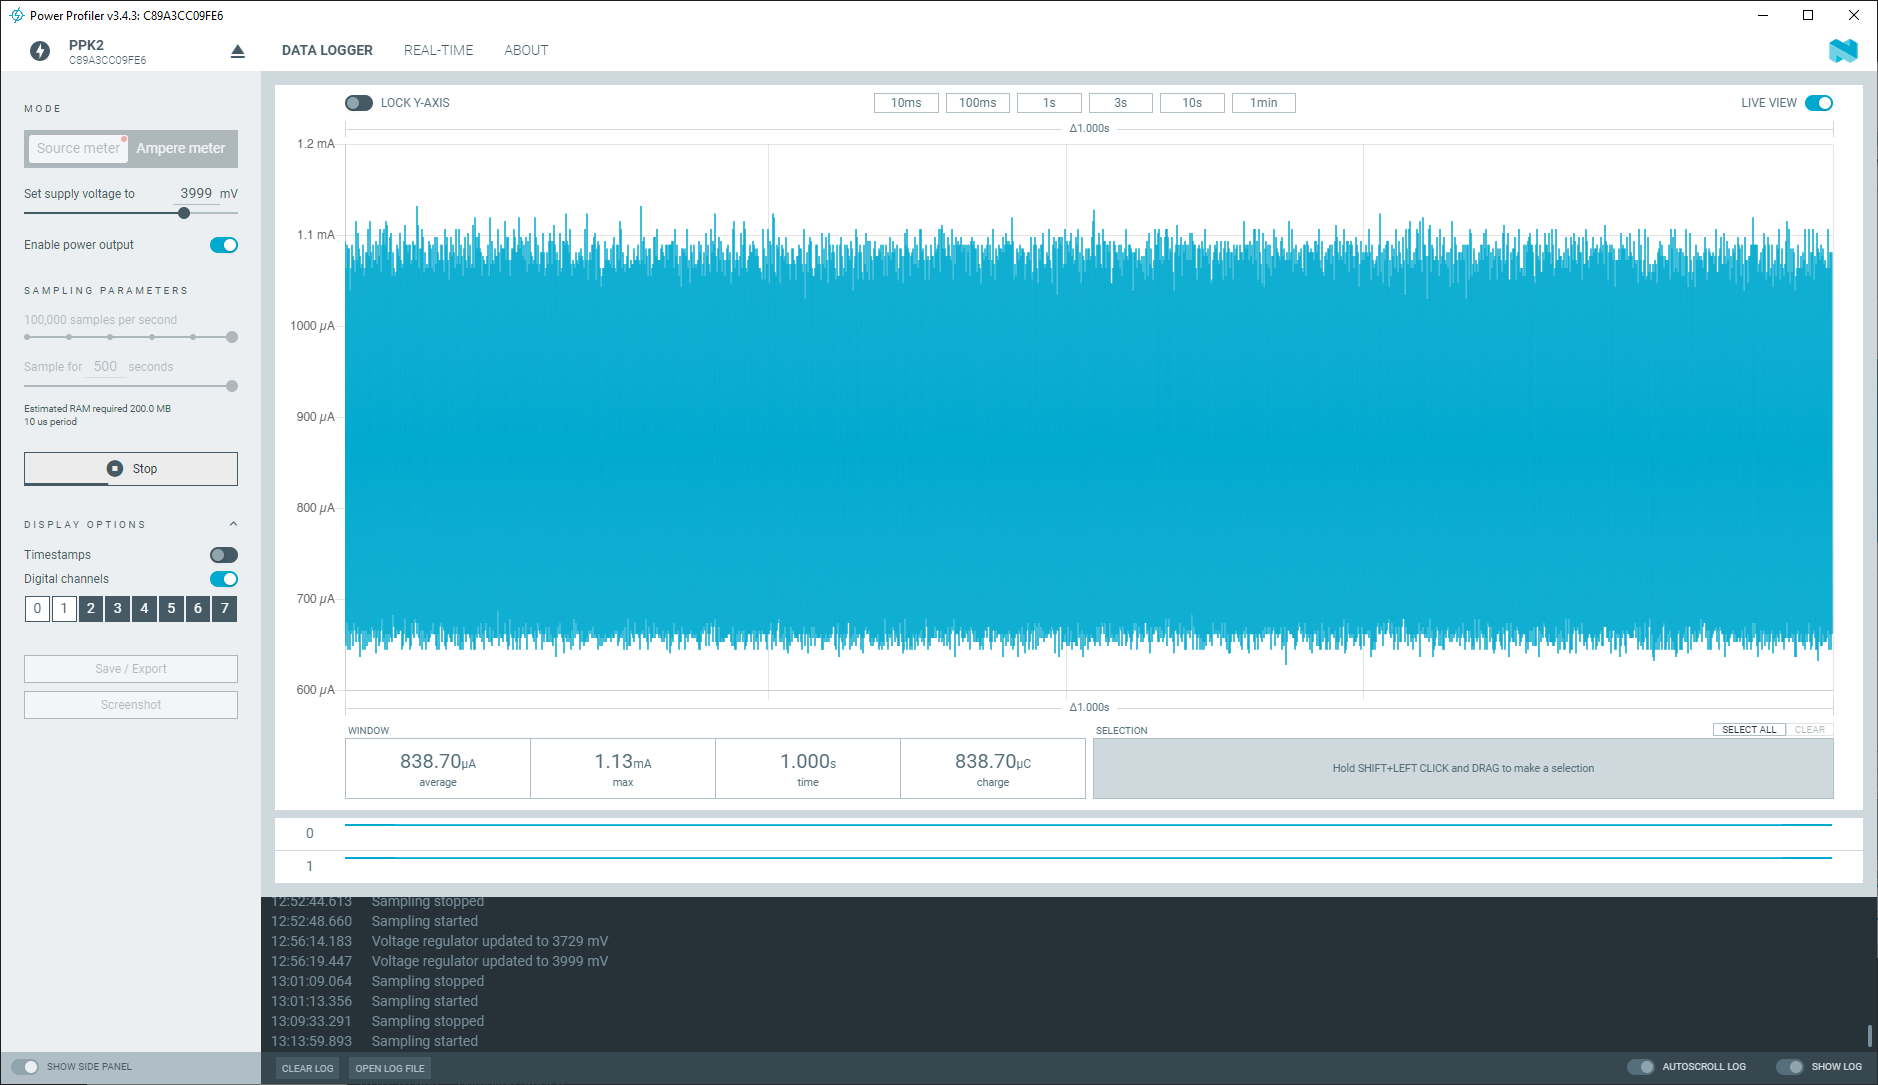
\includegraphics[width=\textwidth]{images/current}
	\caption{Current measurements with the Power Profiler II}
	\label{fig:current}
\end{figure}

\subsection{Telemetry}

For the system to receive commands from the main flight computer of the rocket, the telemetry system is designed to be compatible. The telemetry link on the main fight computer of the rocket is based around \acrlong{fhss} and was developed by the author.

\subsubsection{Hopping Pattern}
The hopping pattern is defined with a password. The password is hashed using a \acrshort{crc}32 algorithm, and the resulting \acrshort{crc} is then used as the seed for a pseudo-random number generator. The generator is run 20 times, defining the hopping pattern. With this method, a password always generates the same hopping pattern. Both the transmitter and receiver require the same password for the transmission to work.

\subsubsection{Synchronization}
The receiver waits on the first frequency until a sync packet is received. The sync packet contains the link \acrshort{crc} to identify the transmission source. If the remote \acrshort{crc} matches the local \acrshort{crc}, the receiver hops to the subsequent frequency, waiting for data. Each data package contains a checksum to validate the contents. The time between packages is measured and used to jump to the next frequency when no package was received in the estimated time frame. A total of 30 hops can be performed without receiving a package before the synchronization is lost. On connection loss, the receiver returns to the first frequency.  

\subsubsection{Package}
Each package contains 14\,Bytes of data but only the state, altitude, and velocity are relevant for the Reefing System. The data is squashed as much as possible to maximize throughput and range.

\begin{figure}[h!]
	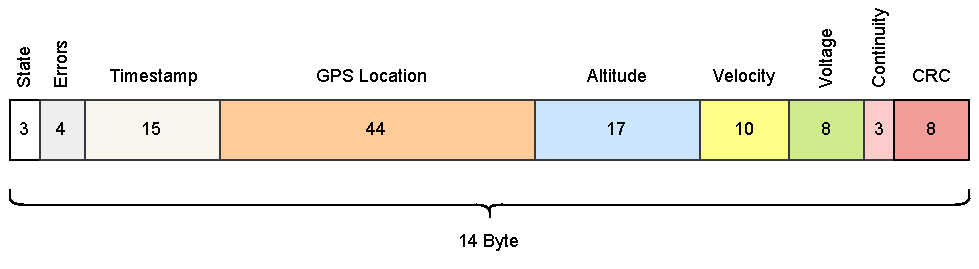
\includegraphics[width=\textwidth]{images/package}
	\caption{Telemetry Data from main flight computer of rocket}
	\label{fig:rf-package}
\end{figure}

\subsubsection{Future use}
Since the main flight computer of the rocket is also still in development and the data is not to be 100\,\% trusted, the Reefing System is only operating in independent mode, meaning the telemetry data is not used at all during flight. However, the device can interface with the main flight computer and use its data for all aspects of flight in the future. 

\subsection{Data Logger}
In order to validate the system and replay flight data, an onboard logging system was added. Since the device is always powered, data is being logged into the \acrshort{ram} of the main \acrshort{mcu}. Each element logged has a size of 5\,B containing the type of data, a timestamp in ms, and the recorded data. With a total reserved size of 64\,kB, it is possible to log 12800 elements per flight.

Only one flight can be recorded on the device. When the system detects liftoff, the previously stored data is overwritten. As soon as the allocated \acrshort{ram} is filled up, the recording is stopped, preventing overflows.  

Four different logging elements were added: the filtered altitude, the estimated altitude, the estimated velocity, and the state transitions. While altitude and velocity data are logged in every user-configured iteration, the state transitions are only logged whenever they occur. 

Maximum log durations of 42 seconds are possible when logging at full speed. The time can be extended for longer flights by changing the logging interval. This can be done through the USB port as explained in Section \ref{usb}.

The logged data can be read out through the \acrshort{usb} port and is then parsed with a jupyter notebook. Using pandas, the data is scaled to \acrshort{si} units and plotly to visualize the recorded flight. Plotly generates interactive plots, allowing for efficient data analysis.

\begin{figure}[h!]
	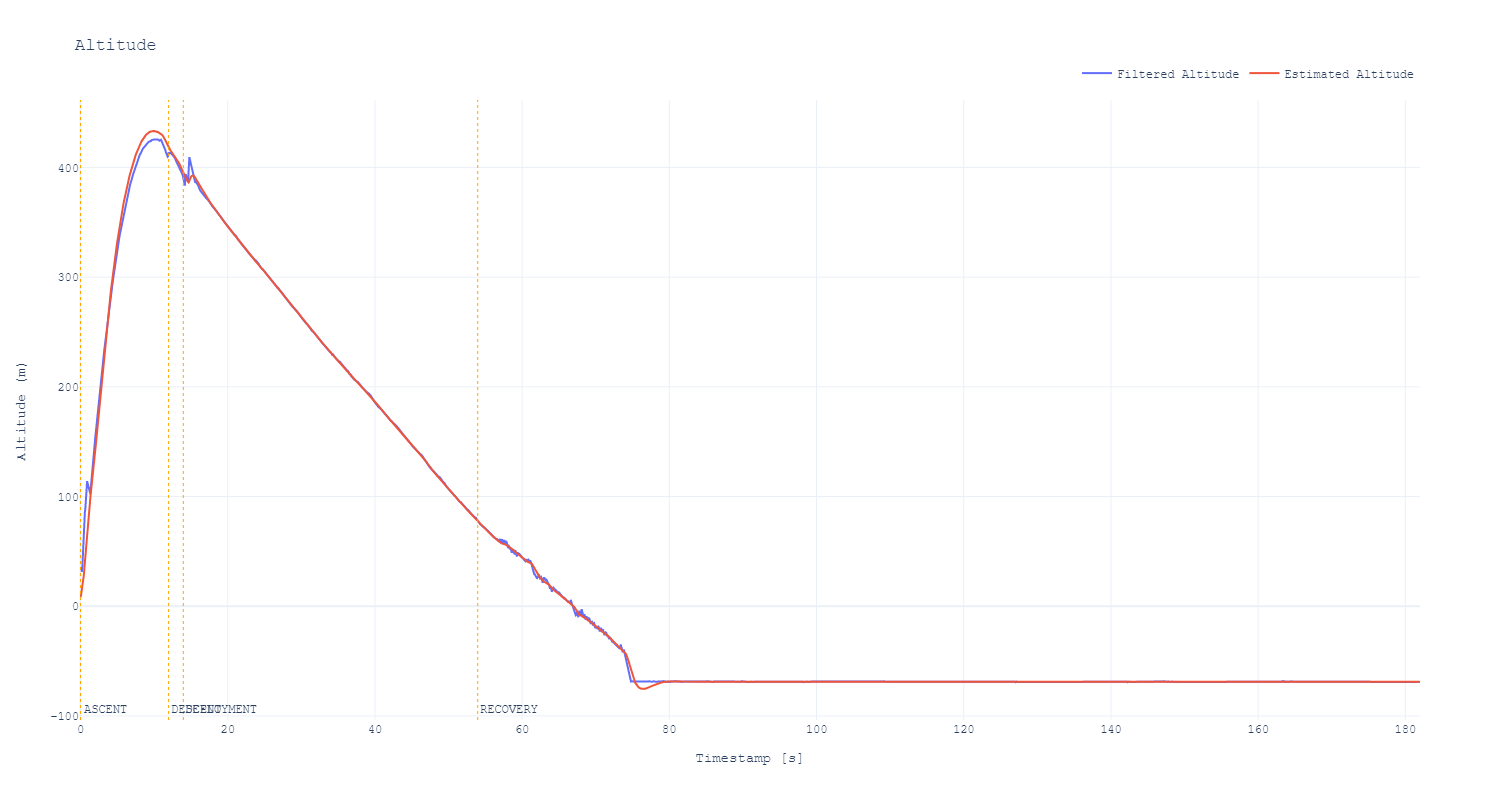
\includegraphics[width=\textwidth]{images/plotly}
	\caption{Visualization of rocket altitude using plotly}
	\label{fig:plotly}
\end{figure}

\newpage

\subsection{USB}\label{usb}
The \acrshort{usb} interface is initialized as a \acrfull{vcp} using the provided libraries from STMicroelectronics. When opening the serial port in a terminal, the device provides diagnostics and battery voltage information. Additionally, it provides a \acrfull{cli} to configure settings on the device, read out data logs, and get general information about the device. The following commands are implemented on the system as presented by the \acrshort{cli}.


\bigskip
\colorlet{mygray}{black!30}
\colorlet{mygreen}{green!60!blue}
\colorlet{mymauve}{red!60!blue}
\begin{lstlisting}[backgroundcolor=\color{gray!10},  
                   basicstyle=\ttfamily,
                   columns=fullflexible,
                   breakatwhitespace=false,      
                   breaklines=true,                
                   captionpos=b,                    
                   commentstyle=\color{mygreen}, 
                   extendedchars=true,              
                   frame=single,                   
                   keepspaces=true,             
                   keywordstyle=\color{blue},      
                   language=C,              
                   numbers=none,                
                   numbersep=5pt,                   
                   numberstyle=\color{blue}, 
                   rulecolor=\color{mygray},        
                   showspaces=false,
                   showstringspaces=false,
                   showtabs=false,                 
                   stepnumber=5,                  
                   stringstyle=\color{mymauve},    
                   tabsize=2,                      
                   title=\lstname,
                   frame=none,
                   xleftmargin = 1cm,
                   framexleftmargin = 1em]
>help
defaults - reset settings to defaults
dump - dump full configuration
get - get variable value
        [cmd_name]
help - display command help
log_enable - enable the logging output
reboot - reboot system
read - print out last recorded flight
save - save configuration
set - change setting
        [<cmd_name>=<value>]
status - show status
version - show version

>

\end{lstlisting}

All configurable settings are shown in the example below. Some of the most important settings are the acceleration threshold used to define the sensitivity of the liftoff detection, the heating element burn duration, and the main altitude. 

\bigskip
\colorlet{mygray}{black!30}
\colorlet{mygreen}{green!60!blue}
\colorlet{mymauve}{red!60!blue}
\begin{lstlisting}[backgroundcolor=\color{gray!10},  
                   basicstyle=\ttfamily,
                   columns=fullflexible,
                   breakatwhitespace=false,      
                   breaklines=true,                
                   captionpos=b,                    
                   commentstyle=\color{mygreen}, 
                   extendedchars=true,              
                   frame=single,                   
                   keepspaces=true,             
                   keywordstyle=\color{blue},      
                   language=C,              
                   numbers=none,                
                   numbersep=5pt,                   
                   numberstyle=\color{blue}, 
                   rulecolor=\color{mygray},        
                   showspaces=false,
                   showstringspaces=false,
                   showtabs=false,                 
                   stepnumber=5,                  
                   stringstyle=\color{mymauve},    
                   tabsize=2,                      
                   title=\lstname,
                   frame=none,
                   xleftmargin = 1cm,
                   framexleftmargin = 1em]
>set
Current settings:
acc_threshold = 35 m/s^2
main_altitude = 100 m
enable_telemetry = 0
enable_preheat = 1
buzzer_volume = 100 %
log_every_n = 5 samples
burn_duration = 35 s
link_phrase = -

>
\end{lstlisting}

The \acrlong{cli} was taken and adapted from the open-source project \gls{betaflight}.

\newpage

\subsection{Persistent Storage}
In order to store configuration settings and retain the information even after a reset, the onboard flash memory is used. The sectors of the microcontroller are not of equal length, therefore the flash mapping was modified to have the user configuration in two dedicated flash sectors each with a length of 16\,kB. As a result, the flash mapping is divided into the following partitions as shown in Table \ref{tab:Flash-Partitions}.

\begin{table}[h]
    \begin{tabular}{ | m{3.15cm} | m{3.7cm}| m{3cm} | m{2.5cm} |} 
      \hline
      \multicolumn{1}{|c|}{\textbf{Name}} & \multicolumn{1}{c|}{\textbf{Type}} & \multicolumn{1}{c|}{\textbf{Memory Address}} & \multicolumn{1}{c|}{\textbf{Size}}\\ \hline
      flash-startup & Startup code and Interrupt Vector Table & \codeword{0x8000000} & 16k \\ \hline
      flash-config & User configuration & \codeword{0x8004000} & 32k \\  \hline
      flash-app & Application & \codeword{0x800C000} & 464k \\  \hline
    \end{tabular}
    \caption{\label{tab:Flash-Partitions}Flash Partitions}
\end{table}

The implementation for reading and writing to the flash is straightforward. Each variable has a fixed length of 32\,bit and is stored with a virtual address, starting at zero. The virtual address is then mapped to the flash memory. In order to change a variable, the whole flash sector needs to be erased and then all stored variables are rewritten. Since the device's configuration is only changed a handful of times, no wear leveling is implemented. Despite contemplation, the implementation of a \acrfull{crc} was not carried out due to time constraints.

\subsection{Sensors}
All sensors on the board are read out, but not all of them are used for the operation. 

\subsubsection{Inertial Measurement Unit}
Only the accelerometer of the \acrshort{imu} is read out, as it is the only data needed for the operation. The maximum acceleration range of 16\,g is selected, and data is read out with a rate of 100\,Hz. Before liftoff, the sensor is put in sleep mode. Acceleration events above 1.5\,g wake the sensor up and generate an interrupt signal for the main microcontroller.

The sensor is used to detect the liftoff of the rocket. If the acceleration on the device is above a user set threshold for over 100\,ms, the finite state machine advances to the ascent phase of the flight. From that point onward, the sensor is not used anymore. 

\subsubsection{Barometer}
The barometer provides accurate pressure and temperature data of the environment. The sensor only provides either the temperature or pressure data for each sample. Therefore the sensor is sampled at a rate of 200\,Hz. Alternating between the temperature and pressure readouts. 

The pressure data is used for the state estimation as explained in Section \ref{state-estimation}.

\newpage

\subsubsection{Thermocouple}
Over \acrshort{spi} the temperature of the thermocouple is readout. 

Initially, the idea of the sensor was to read the temperature of the heating element and build a controller around it. Unfortunately, the thermocouple placement turned out to be extremely difficult, and the temperature measured did not reflect the actual temperature of the heating element. Each device would need to be calibrated for an accurate temperature readout, and a displacement of the thermocouple would result in bad measurements. For that reason, the thermocouple is not used in the software.  

\subsubsection{Light Sensor}
A light sensor implementation was added, where the sensor can be used as a binary signal. The analog value from the sensor is converted using the microcontrollers \acrshort{adc}. 

Before ejection of the parachute, the Reefing System is in the dark. In that state, the sensor can be calibrated to detect a change in brightness. The change translates to the ejection of the parachute and can be used for the finite state machine. As of now, the sensor is not taken into account by the \acrshort{fsm}.

\subsection{State Estimation}\label{state-estimation}
In order to get accurate altitude and vertical velocity information, a state estimation is implemented. The Figure \ref{fig:state-est} provides an overview of the data flow.
\begin{figure}[h!]
	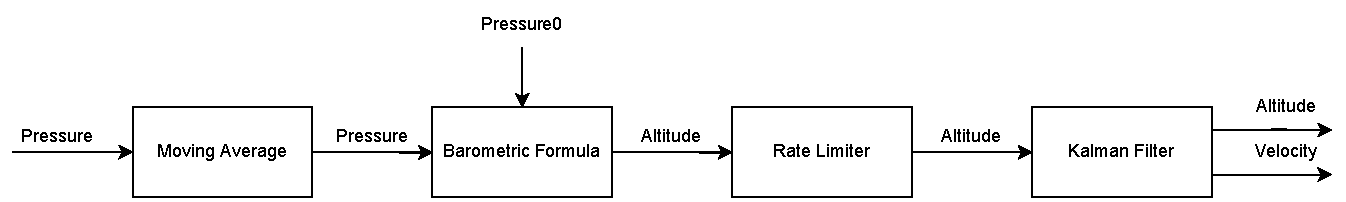
\includegraphics[width=\textwidth]{images/state-est}
	\caption{Overview of State Estimation Data Flow}
	\label{fig:state-est}
\end{figure}

\subsubsection{Moving Average}
The only sensor used for the state estimation is the barometer. In order to smooth out the data before passing it on, a moving average filter is implemented. For the filter, $k$ samples are summed up and then divided by their size $k$. The mean over the last $k$ data-points is denoted as $SMA_{k}$ and calculated as:

\begin{equation}
    SMA_{k} = \frac{1}{k}\sum _{i=n-k+1}^{n}p_{i}
\end{equation}

A filter size of 8 was chosen, as it is ideal for efficient operation. The division needed can be replaced with right shift operations on the hardware as the data is stored as an unsigned integer.

\subsubsection{Measurement}
The barometric air pressure is converted to the altitude above ground level. Because weather conditions affect altitude calculations, the pressure and temperature at sea level must be known. Since that data is not available, the \acrshort{icao} Standard Atmosphere model is used to calculate the relative altitude from liftoff. \acrshort{icao} defines the air temperature to be 15\,$^{\circ}$C below an altitude of 11\,km. Before liftoff, the system continuously takes air pressure readings, averages them, and stores it as the initial air pressure $P_0$. Using the barometric formula, the relative altitude can be calculated.\cite{atmosphere}

\begin{equation}
    h = \frac{T_0}{L}\times{}\left({\frac{P}{P_0}}^{\frac{-R\times L}{g\times M}} - 1\right)
\end{equation}

where
\begin{itemize}
    \item $h$ is the relative altitude in m;
    \item $T_0$ is the air temperature at sea level in K;
    \item $L$ is the standard temperature lapse $= -0.0065\frac{K}{m}$;
    \item $P$ is the current air pressure in Pa;
    \item $P_0$ is the air pressure at liftoff altitude in Pa;
    \item $R$ is the universal gas constant $= 8.31432 \frac{Nm}{molK}$;
    \item $g$ is the gravitational constant $= 9.81 \frac{m}{s^2}$;
    \item $M$ is the molar mass of Earth's air $= 0.0289644 \frac{kg}{mol}$.
\end{itemize}

Before passing the air pressure data through the formula, it is converted into a 32-bit floating-point number.

\subsubsection{Rate limiter}
In order to eject parachutes from a rocket body, the section where the parachute, and consequently the Reefing System, is located gets pressurized. These pressure spikes usually last for one to two seconds. For that reason, a rate limiter is implemented. The rate limiter prevents the altitude from dropping suddenly, thus preventing the Kalman filter from receiving bad data points. An implementation of a median filter was considered, but since the pressure spikes can last multiple seconds, it was decided against that option. 

Rockets can reach incredibly high speeds while ascending. Therefore the ascent rate is not limited by the rate limiter. For the descent, on the other hand, the rate limiter is set to -25\,m/s. In a nominal flight, descent rates will never surpass that threshold. Therefore, if the measured descent rate is less than the falling slew rate of -25\,m/s the output is calculated as:

\begin{equation}
    y(i) = \Delta t \times F + y(i-1) 
\end{equation}

where

\begin{itemize}
    \item $F$ is the falling slew rate;
    \item $\Delta t$ is time between samples;
\end{itemize}

\newpage

\subsubsection{Kalman Filter Design}

Kalman filters are used to estimate states based on linear dynamical systems. In order to estimate the current altitude and vertical velocity of the rocket a linear Kalman Filter was deployed. The state space of the filter is described as follows:
\begin{equation}
    x = \begin{bmatrix}h\\v\end{bmatrix}
\end{equation}
where
\begin{itemize}
    \item $h$ is the position (altitude) of the rocket;
    \item $v$ is the velocity of the rocket which can also be described as the derivative of the position $\dot{h}$.
\end{itemize}

We assume that between the previous $(k-1)$ and the current timestep $k$ constant accelerations $w_a$ act upon the rocket. The acceleration is normally distributed, with mean 0 and standard deviation $w_R \sim \mathcal{N} (0, \sigma_R)$. This process noise is used to tune the dynamics of the filter, which was done using a simulation and flight data of previous rocket flights. More information can be found in Section \ref{filter-tuning}.

From Newton's laws of motion we can conclude that:

\begin{equation}
    \dot{x} = Ax + Gw_a
\end{equation}

\begin{equation}
    \dot{x} = \begin{bmatrix}v\\a\end{bmatrix} =  \begin{bmatrix}0 & 1\\ 0 & 0\end{bmatrix} \begin{bmatrix}h\\v\end{bmatrix} + \begin{bmatrix}0\\1\end{bmatrix}w_a
\end{equation}

Since no control inputs are known, the model is simplified by removing the $B$ matrix.

For the measurement model we assume a Gaussian white noise for the sensor noise $w_R \sim \mathcal{N} (0, \sigma_R)$.
The measurement model is defined as:
\begin{equation}
    z = Hx + w_R
\end{equation}
\begin{equation}
    z = \begin{bmatrix}1 & 0\end{bmatrix} \begin{bmatrix}h\\v\end{bmatrix} + w_R
\end{equation}

Afterward, the model was discretized and implemented on the hardware. The discretization process and implementation can be found in Appendix \ref{apx:kalman}

\chapter{Validation \& Testing}

\section{Cutting Tests}
To validate the line cutter, a series of cutting tests were performed. 

\begin{figure}[h!]
    \centering
	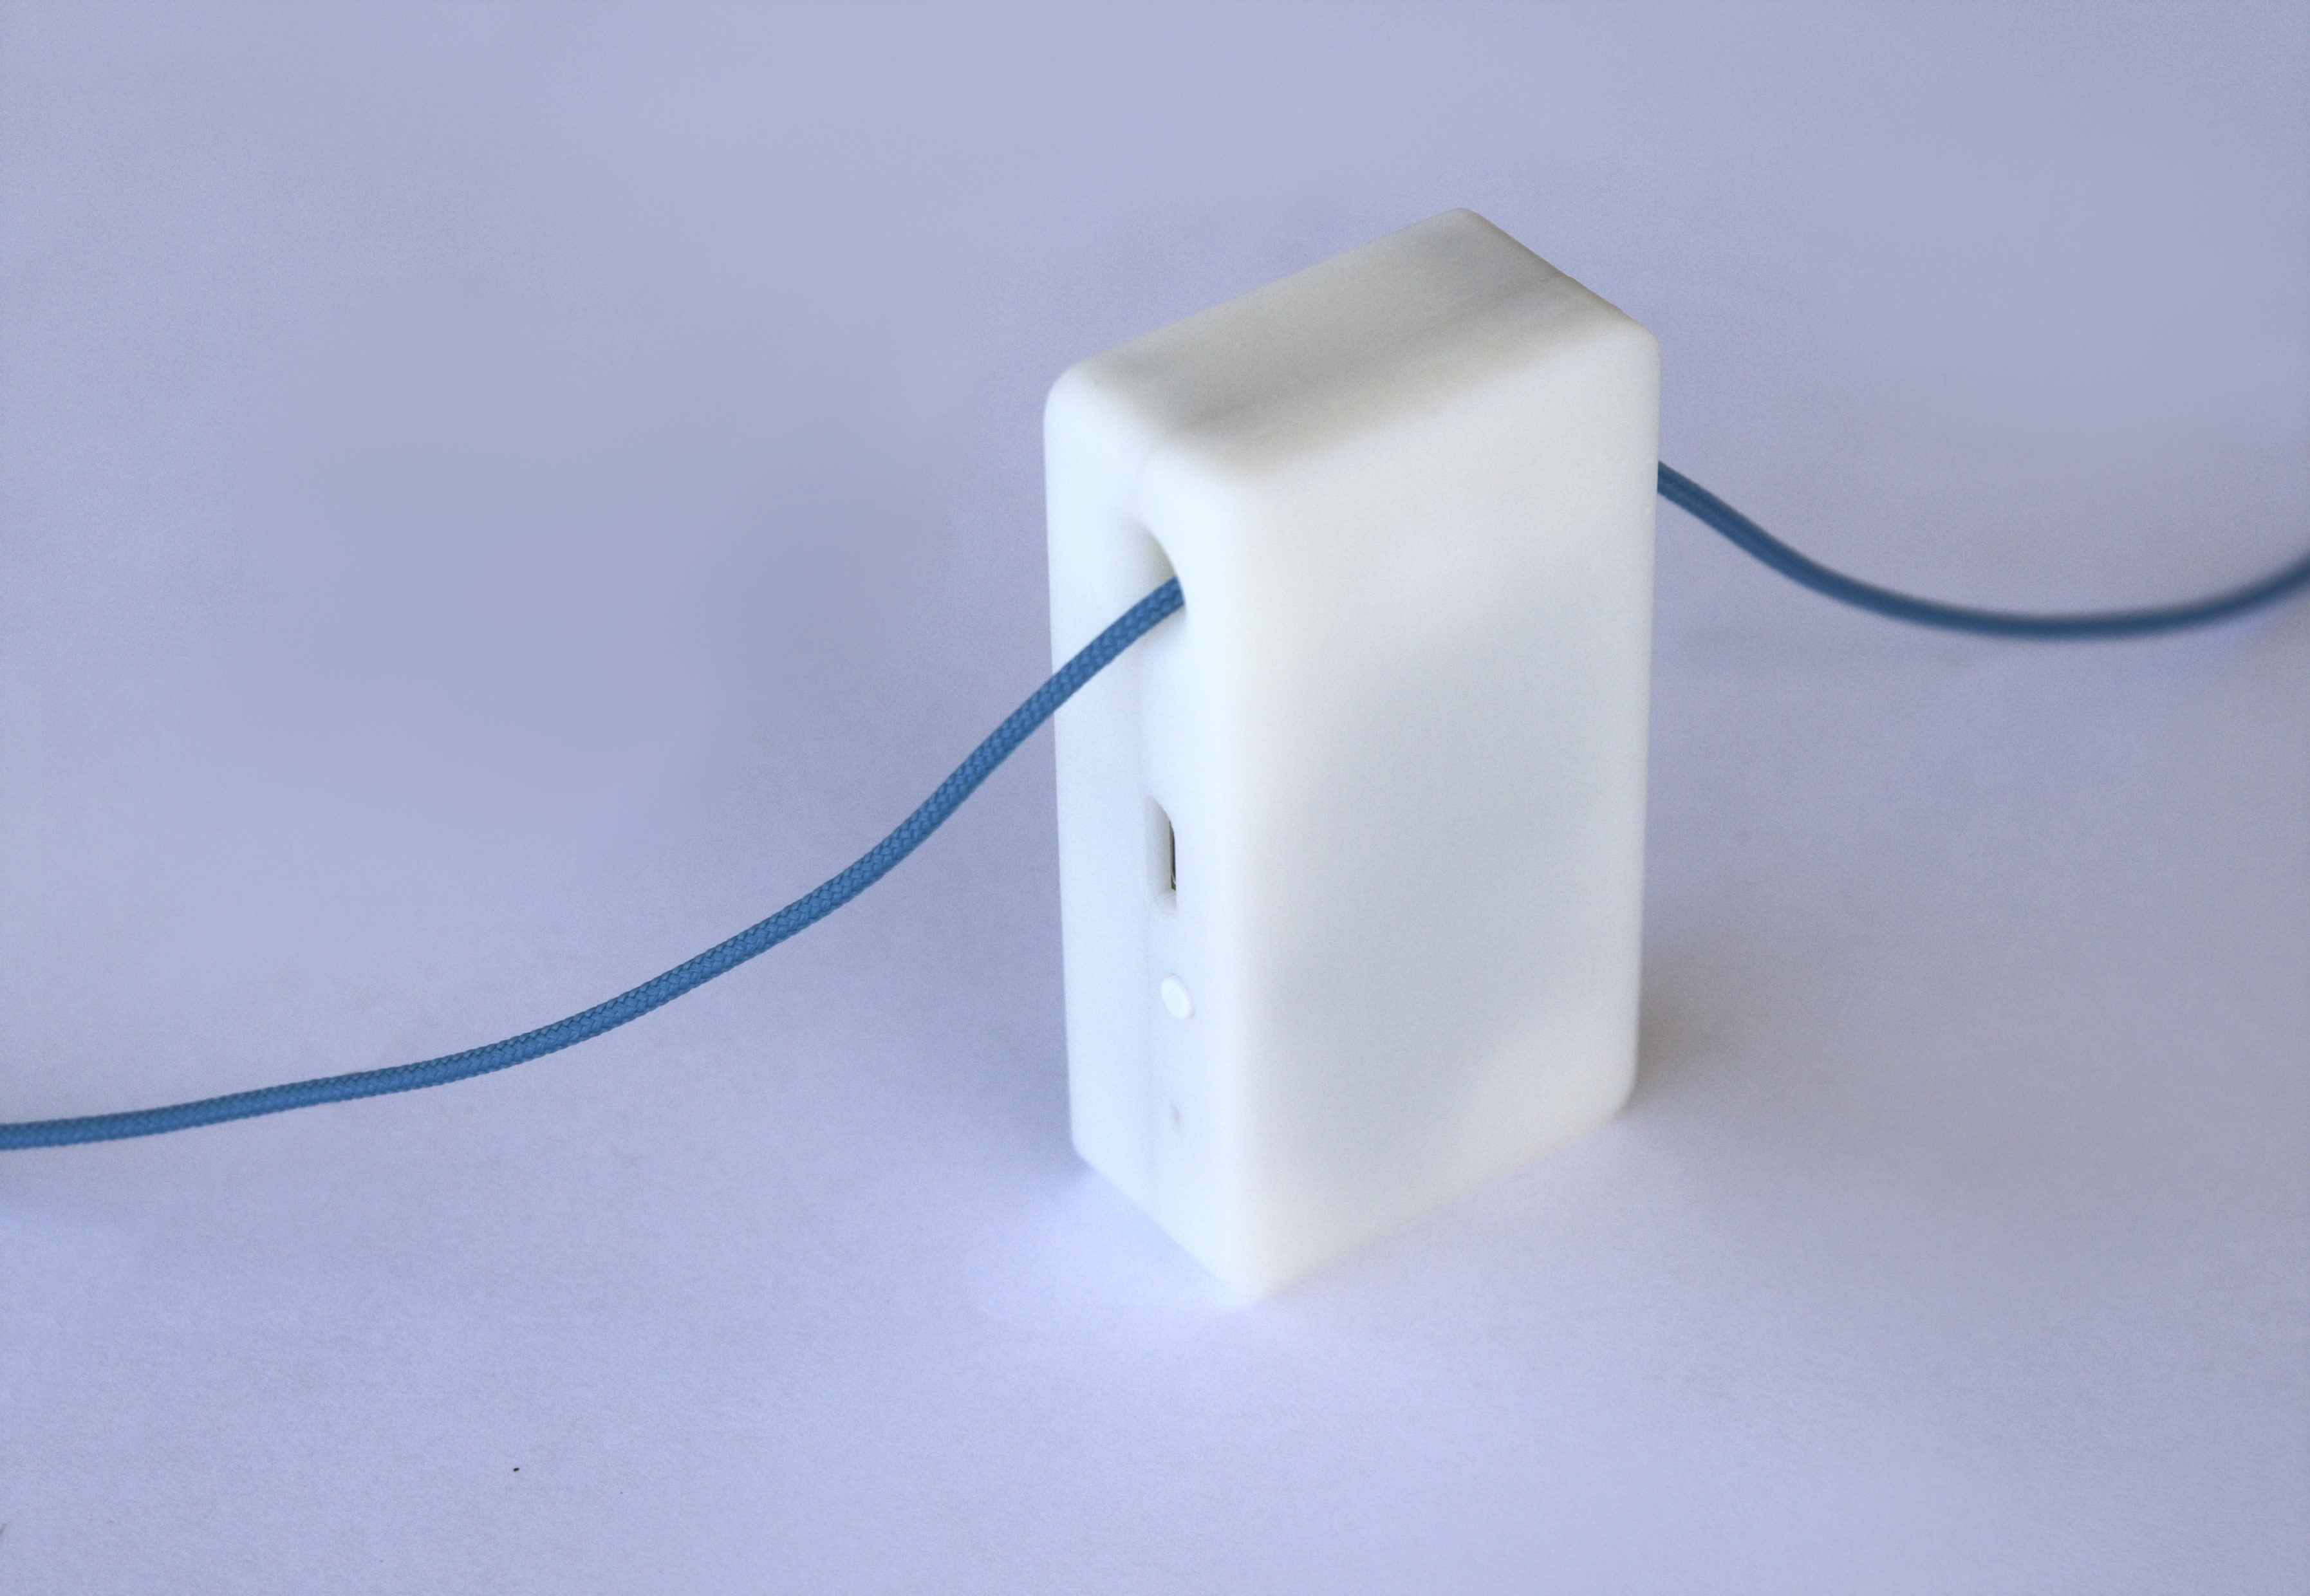
\includegraphics[width=8cm]{images/cutting-test}
	\caption{Cutting tests performed with the Reefing-System}
	\label{fig:cutting-test}
\end{figure}

\subsubsection{Scope of Test}
The scope of the cutting tests is to work out the cutting speed and repeatability. In particular, the following functions were tested:
\begin{itemize}
    \item Temperature of the ceramic heating element
    \item Time to cut reefing line 
    \item Variance in cutting time
\end{itemize}

\subsubsection{Acceptance criteria}
The test is successful if
\begin{itemize}
    \item The reefing line is always cut
    \item The time to cut, for the same setup, stays within a standard deviation of 5 seconds 
\end{itemize}

\subsection{Test Setup}
The Reefing System powered the heating element with a fully charged battery for both tests, and the heating element voltage was set to the maximum 12.2\,V. All tests were performed at an ambient temperature of 24\,$^\circ$C.

\subsubsection{Temperature measurement}
In order to generate a temperature curve of the heating element, a multimeter with a thermocouple was used. The thermocouple was firmly pressed against the surface of the heating element to get a reading close to the actual surface temperature. With a camera, the multimeter's display was recorded. The video was then used to get the data points. This test was repeated three times to get a better estimate. 

\subsubsection{Cutting Tests}
For the cutting tests, a paracord made out of nylon was used. The lines had a diameter of 1.4\,mm and 2.0\,mm. For testing the impact of force on the reefing line, a weight was added to one side of the paracord and suspended in air. The other end was tied down on a table. The time from the initiation of the cut to the separation was measured with a stopwatch. 

\subsection{Results}
\subsubsection{Temperature measurement}
A temperature curve was plotted using Python and matplotlib. The temperature increase is quite linear initially but drops off towards the end of the 30-second testing duration. As seen in Figure \ref{fig:temperature}, the experiment was repeated three times, and the corresponding temperature curves are relatively similar. A maximum temperature of 360\,$^\circ$C can be expected after 30 seconds.

\begin{figure}[h!]
	\centering
	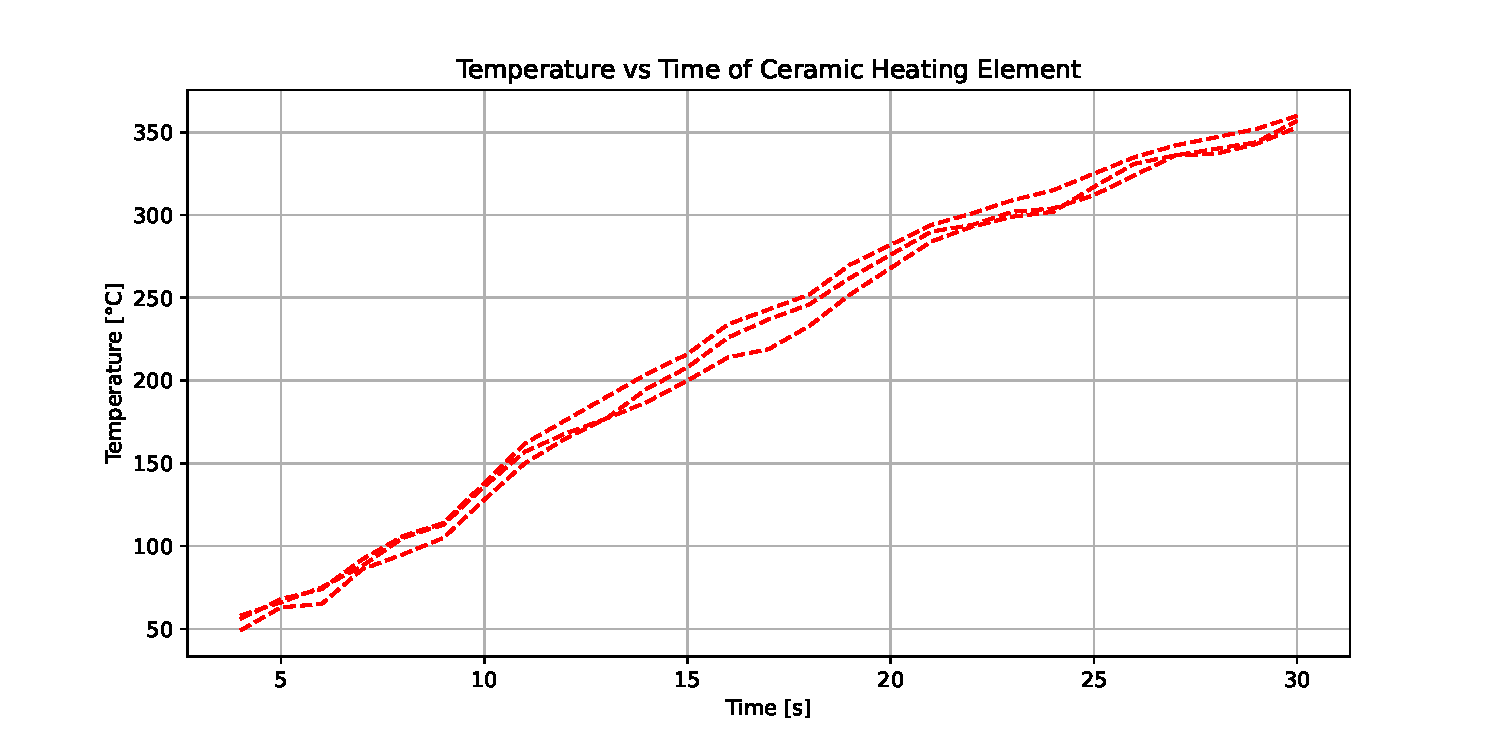
\includegraphics[width=\textwidth]{plots/temperature}
	\caption{Temperature plot of ceramic heating element}
	\label{fig:temperature}
\end{figure}

\subsubsection{Cutting Tests}
Four series of cutting tests were performed. For each series, six tests were performed to get a valid standard deviation. From the tests performed, it can be concluded that the standard deviation is a lot smaller than initially expected. Even when taking into account all measurements from both lines and forces, the standard deviation is still bellow 1.5\,s. 

\begin{table}[h]
    \centering
    \begin{tabular}{ m{4cm} | m{1.5cm} | m{1.5cm} } 
      \hline
      Force                 & \multicolumn{1}{c}{0.098\,N} & \multicolumn{1}{|c}{9.8\,N}  \\ \hline
      Time Delay            & \multicolumn{1}{c}{22.2}    & \multicolumn{1}{|c}{20.8}       \\
                            & \multicolumn{1}{c}{22.6}    & \multicolumn{1}{|c}{21.4}       \\
                            & \multicolumn{1}{c}{23.6}    & \multicolumn{1}{|c}{20.9}       \\
                            & \multicolumn{1}{c}{23.0}    & \multicolumn{1}{|c}{21.4}       \\
                            & \multicolumn{1}{c}{23.5}    & \multicolumn{1}{|c}{20.8}       \\
                            & \multicolumn{1}{c}{23.3}    & \multicolumn{1}{|c}{20.4}       \\
                            & \multicolumn{1}{c}{}        &  \multicolumn{1}{|c}{}          \\
      Mean                  & \multicolumn{1}{c}{23.06}   &\multicolumn{1}{|c}{20.95}      \\
                            & \multicolumn{1}{c}{}        &  \multicolumn{1}{|c}{}          \\
      Standard Deviation    & \multicolumn{1}{c}{0.572}   &\multicolumn{1}{|c}{0.482}      \\
    \end{tabular}
    \caption{\label{tab:nylon-2}Cutting tests performed with a 2.0\,mm nylon line}
\end{table}

\begin{table}[h]
    \centering
    \begin{tabular}{ m{4cm} | m{1.5cm} | m{1.5cm} } 
      \hline
      Force                 & \multicolumn{1}{c}{0.098\,N} & \multicolumn{1}{|c}{9.8\,N}  \\ \hline
      Time Delay            & \multicolumn{1}{c}{20.2}    & \multicolumn{1}{|c}{18.7}       \\
                            & \multicolumn{1}{c}{21.6}    & \multicolumn{1}{|c}{18.5}       \\
                            & \multicolumn{1}{c}{19.4}    & \multicolumn{1}{|c}{19.6}       \\
                            & \multicolumn{1}{c}{20.8}    & \multicolumn{1}{|c}{18.9}       \\
                            & \multicolumn{1}{c}{20.9}    & \multicolumn{1}{|c}{19.1}       \\
                            & \multicolumn{1}{c}{21.4}    & \multicolumn{1}{|c}{20.0}       \\
                            & \multicolumn{1}{c}{}        &  \multicolumn{1}{|c}{}          \\
      Mean                  & \multicolumn{1}{c}{20.70}   &\multicolumn{1}{|c}{19.13}      \\
                            & \multicolumn{1}{c}{}        &  \multicolumn{1}{|c}{}          \\
      Standard Deviation    & \multicolumn{1}{c}{0.811}   &\multicolumn{1}{|c}{0.568}      \\
    \end{tabular}
    \caption{\label{tab:nylon-14}Cutting tests performed with a 1.4\,mm nylon line}
\end{table}

\subsubsection{Test success}
The cutting and heating tests confirmed the system's reliability and exceeded the required standard deviation substantially. These numbers should not be taken as facts, as conditions during flight could impact performance. For example, airflow and line movement can increase the time to separation.

\newpage

\section{Simulation}
Before implementing the state estimation on the hardware, a simulation was written in Python to validate the performance.

\subsubsection{Scope of Test}
The simulation is used to validate the state estimation model and to tune the gains of the Kalman filter. In detail, the following functions should be tested:
\begin{itemize}
    \item Correctness of Kalman filter model
    \item Test finite state machine 
    \item Correctness of deployment altitude
\end{itemize}

\subsubsection{Acceptance criteria}
The test is successful if
\begin{itemize}
    \item The altitude and velocity estimation is accurate
    \item The Kalman filter can be tuned to acceptable levels
    \item The finite state machine working as expected
    \item The estimated cutting point is within 50\,m of the targeted altitude
\end{itemize}

\subsection{Test Setup}
For the test, the entire state estimation algorithm and the finite state machine were implemented in Python. Data from previous rocket flights are used for the simulation. Different flight profiles can be passed through to determine the system's effectiveness. The main altitude was set to 100 meters above ground level, and the burn duration is estimated to be 10 seconds.


In order to compare the estimations, raw data and moving averages are displayed in the same plot. The derivative of a moving average was taken for the velocity estimation since raw data had way too much noise.

The data used for the simulations were collected from previous rocket flights from ARIS using the same barometer. Therefore the noise and accuracy closely match the expected data from the Reefing System. Furthermore, the data is collected at 100\,Hz, which also matches the sampling speed on the Reefing System.  

\newpage

\subsection{Results}

\subsubsection{Kalman filter tuning}\label{filter-tuning}
Two parameters of the Kalman filter are used to tune the dynamics of the filter. The gain $R$, the altitude measurement covariance $\sigma_R$ and $Q$, the acceleration covariance $\sigma_a$. 

By analyzing previous flight data and the datasheet from the barometer, a measurement covariance of 5\,m was chosen. The acceleration covariance was experimentally selected by running a series of simulations. As shown in Figure \ref{fig:tune-velocity} it can be observed that the lower the covariance is, the smoother or less responsive the velocity estimation becomes. A smooth velocity estimation is beneficial for the application as it improves the deployment estimate. Thus a value of 5\,{m/s}$^2$ was selected. While the velocity is more irregular than lower $Q$ values, the altitude estimate, as seen in Figure \ref{fig:tune-altitude}, is closer to the real world.   

\begin{figure}[h!]
	\centering
	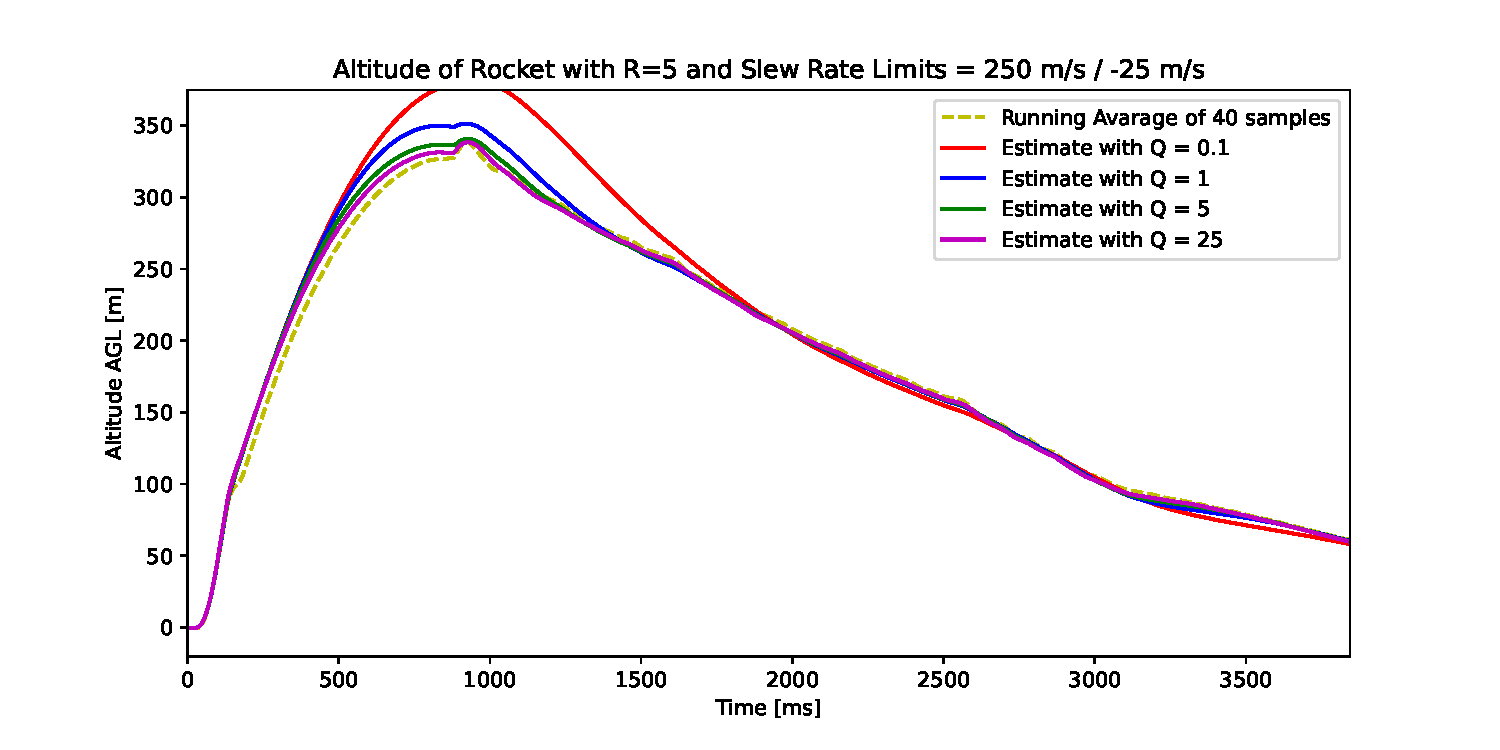
\includegraphics[width=\textwidth]{plots/altitude-tune}
	\caption{Altitude plot of flight simulation}
	\label{fig:tune-altitude}
\end{figure}

\begin{figure}[h!]
	\centering
	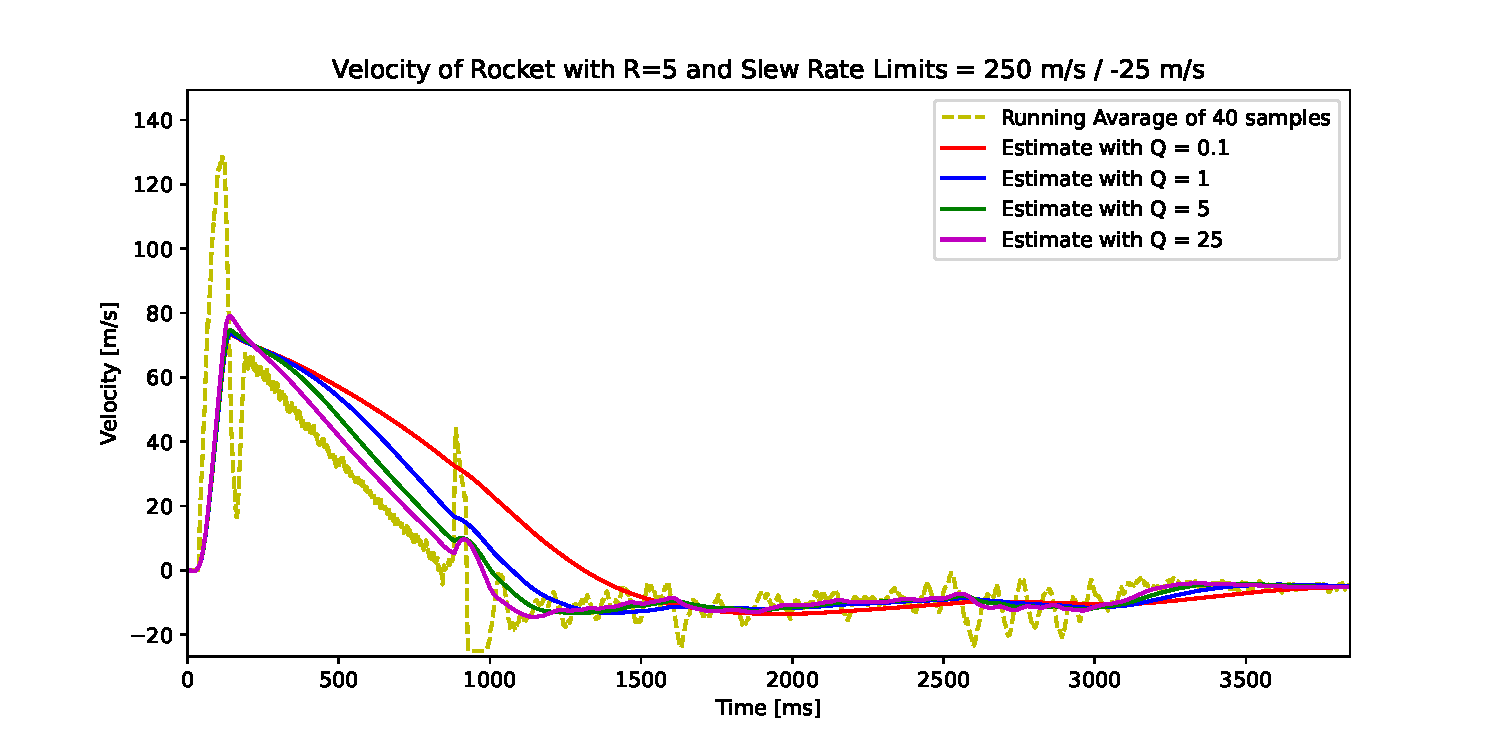
\includegraphics[width=\textwidth]{plots/velocity-tune}
	\caption{Velocity plot of flight simulation}
	\label{fig:tune-velocity}
\end{figure}

\subsubsection{Test success}
The state estimation is working as expected, and especially the velocity estimation is significantly improved over the running average as shown in Figure \ref{fig:sim-velocity}. The state estimation and the finite state machine make it possible to accurately predict the flight phases and the point where the heating element gets turned on. The estimated cutting point matches the requested altitude closely. The simulation made it possible to find an appropriate filter tune, and the Kalman filter matches the model. 

\begin{figure}[h!]
	\centering
	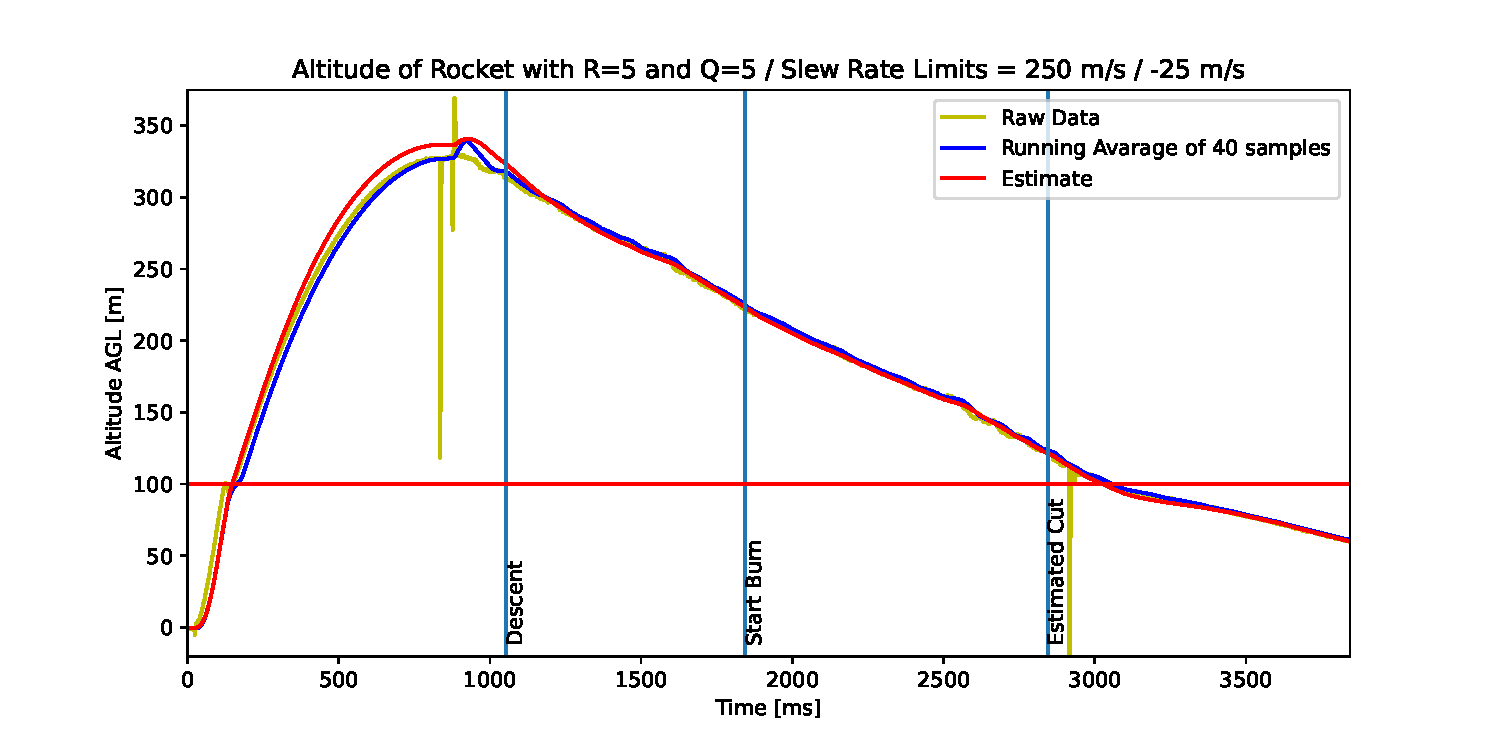
\includegraphics[width=\textwidth]{plots/sim-altitude}
	\caption{Altitude plot of flight simulation}
	\label{fig:sim-altitude}
\end{figure}

\begin{figure}[h!]
	\centering
	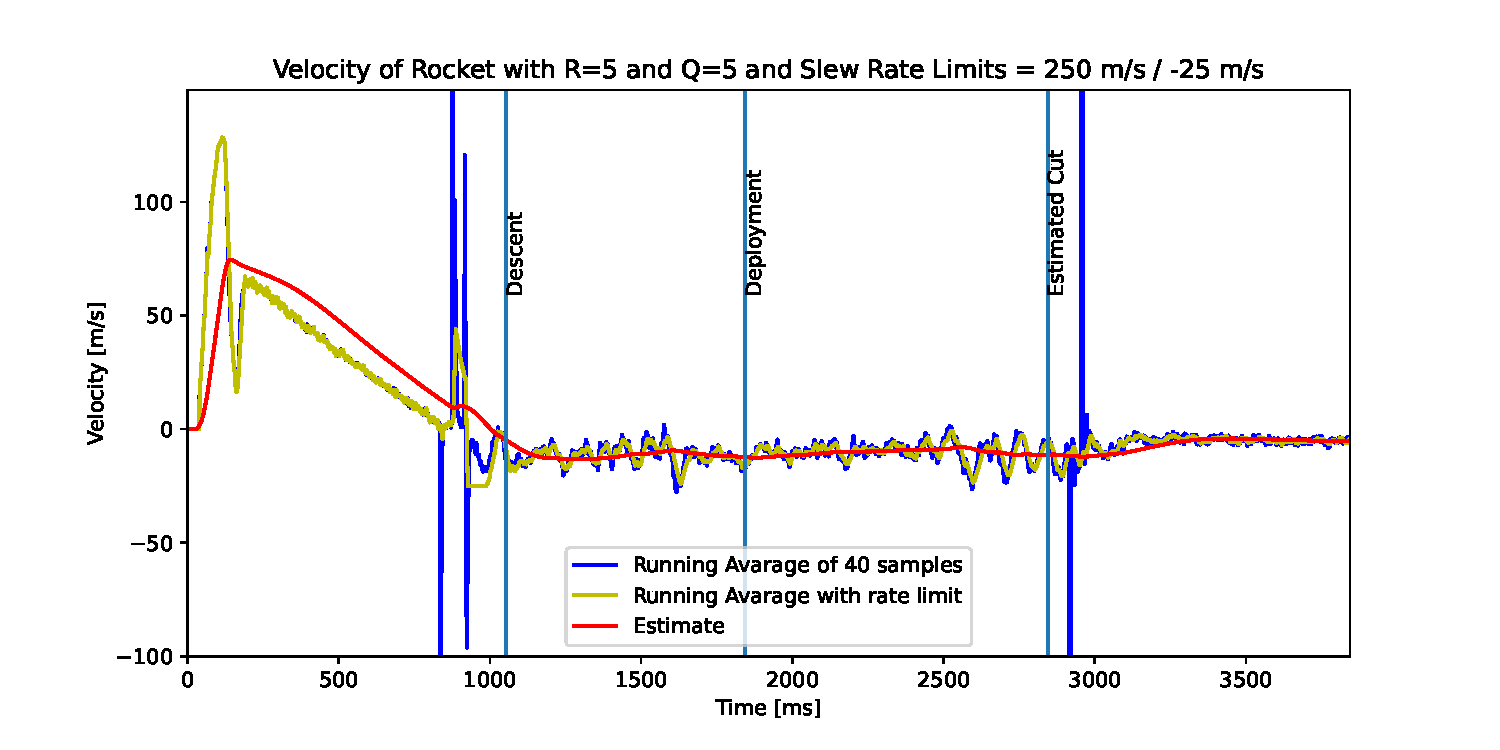
\includegraphics[width=\textwidth]{plots/sim-velocity}
	\caption{Velocity plot of flight simulation}
	\label{fig:sim-velocity}
\end{figure}

\newpage

\section{Firmware Validation}
To validate that all tasks are executed on time and that no stack overflow occurs, the \acrshort{rtos} was traced.

\begin{figure}[h!]
    \centering
	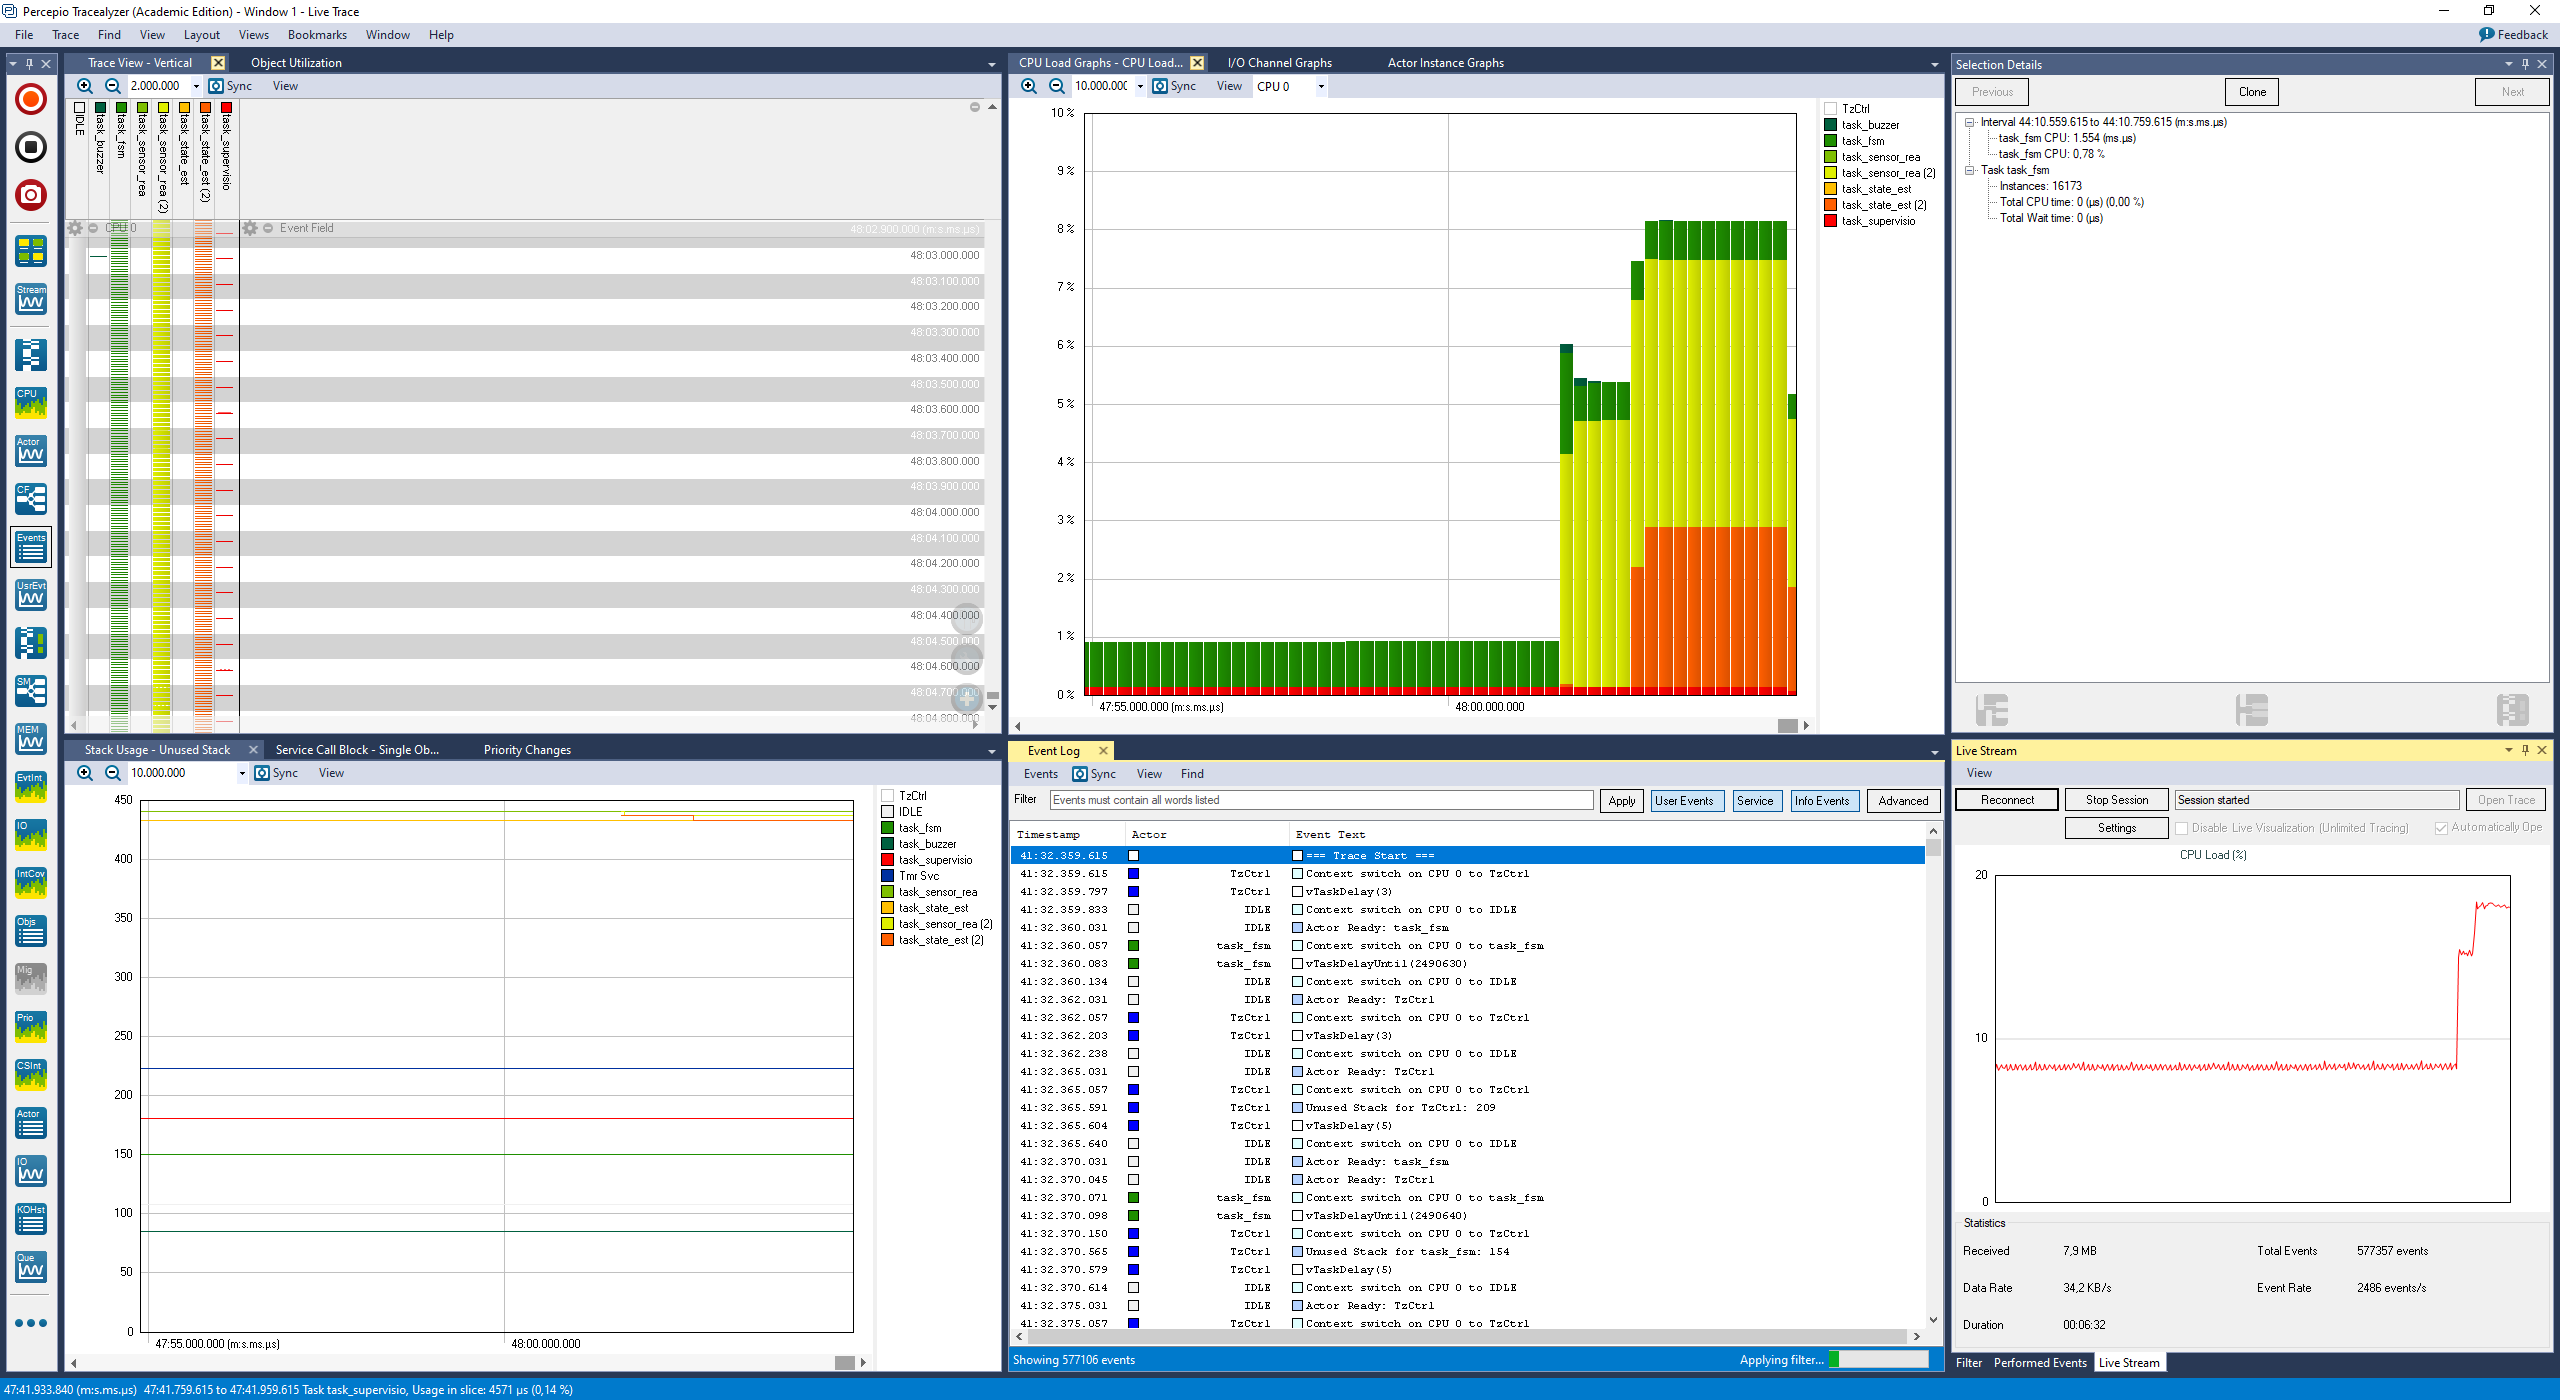
\includegraphics[width=10cm]{images/tracealyzer}
	\caption{Overview of trace views in Tracealyzer 4}
	\label{fig:tracealyzer}
\end{figure}

\subsubsection{Scope of Test}
The scope of the firmware validation is to verify the operation during all phases of flight. In detail, the following functions should be tested:
\begin{itemize}
    \item Task execution timings
    \item \acrshort{cpu} utilization
    \item Task stack usage
    \item Dynamic task starting and stopping
\end{itemize}

\subsubsection{Acceptance criteria}
The test is successful if
\begin{itemize}
    \item All task execution timings are as expected
    \item The \acrshort{cpu} usage stays bellow 75\,\%
    \item All tasks have at least 64 integers free stack
    \item Dynamic starting and stopping of the tasks works without any issues
\end{itemize}

\subsection{Test Setup}
Tracealyzer is a solution for visual trace diagnostics, giving embedded software developers insight into the runtime world. This tool allows for easier debugging of system-level issues and helps improve the software's design and performance. For the validation, a framework was added to the firmware to print out trace data over the \acrshort{usb} port. Percepio, the developer of Tracealyzer, provides the framework. While the trace is enabled, the \acrshort{cli} is disabled to not generate package collisions over the \acrshort{usb}.

\subsection{Results}
\subsubsection{Measurements and Observations}
From the \acrshort{cpu} load graph, it is easily recognizable that there is more than enough headroom for additional processing. During the flight, the maximum reached \acrshort{cpu} usage does not exceed 9\,\%. As shown in Figure \ref{fig:cpu-usage} the two tasks that require the most time to execute are the state estimation and sensor read task. This behavior is expected, as the sensor readout is done with all blocking functions and is therefore bound to \acrshort{spi} speeds. The state estimation requires the second-longest time to execute. The execution time for the state estimation is mainly the processing time for all the filters. The buzzer task is not fixed to a sampling frequency. Therefore it only utilizes \acrshort{cpu} time whenever the buzzer is beeping. The time it takes to print out the trace information is contained in the TzCtrl generated by the Tracealyzer framework and is not enabled in the trace.  

\begin{figure}[h!]
    \centering
	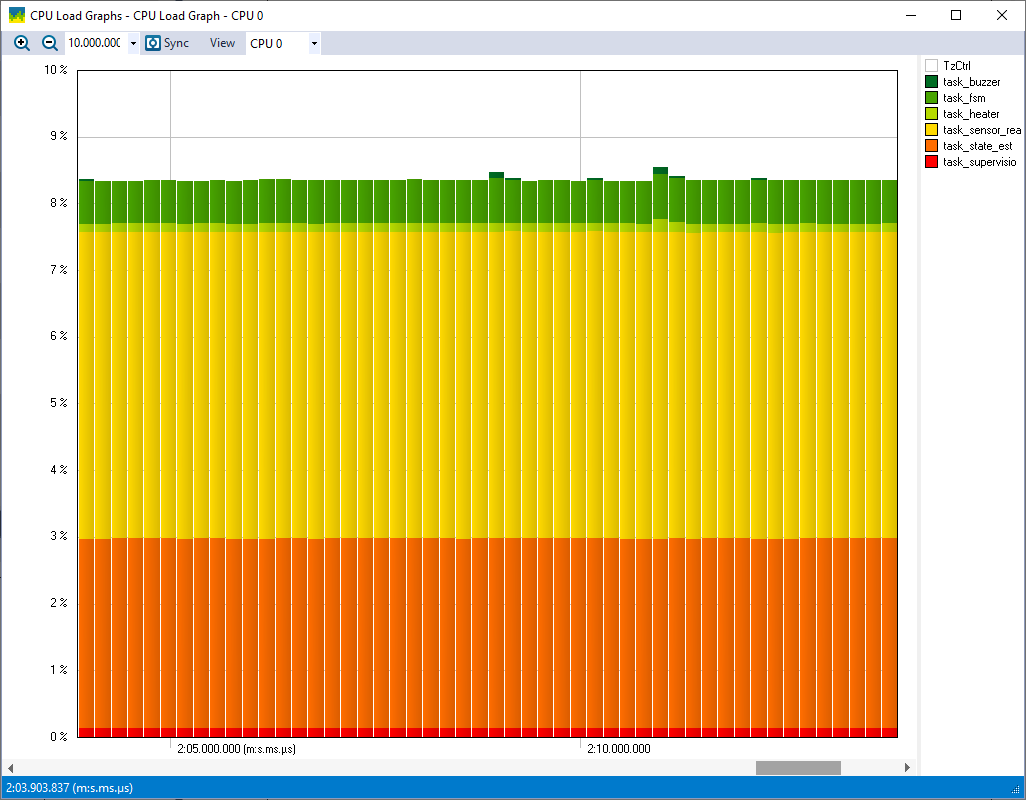
\includegraphics[width=7.8cm]{images/cpu-usage}
	\caption{CPU usage during flight with all tasks running}
	\label{fig:cpu-usage}
\end{figure}

The dynamically starting and stopping of the tasks were tested by switching the device from the idle mode to the ready mode and back. As soon as the state is changed, all required tasks are started, as shown in Figure \ref{fig:cpu-start}. The state estimation does not execute immediately after it is started, allowing for all the sensors to be initialized and read out at least once.

\begin{figure}[h!]
    \centering
	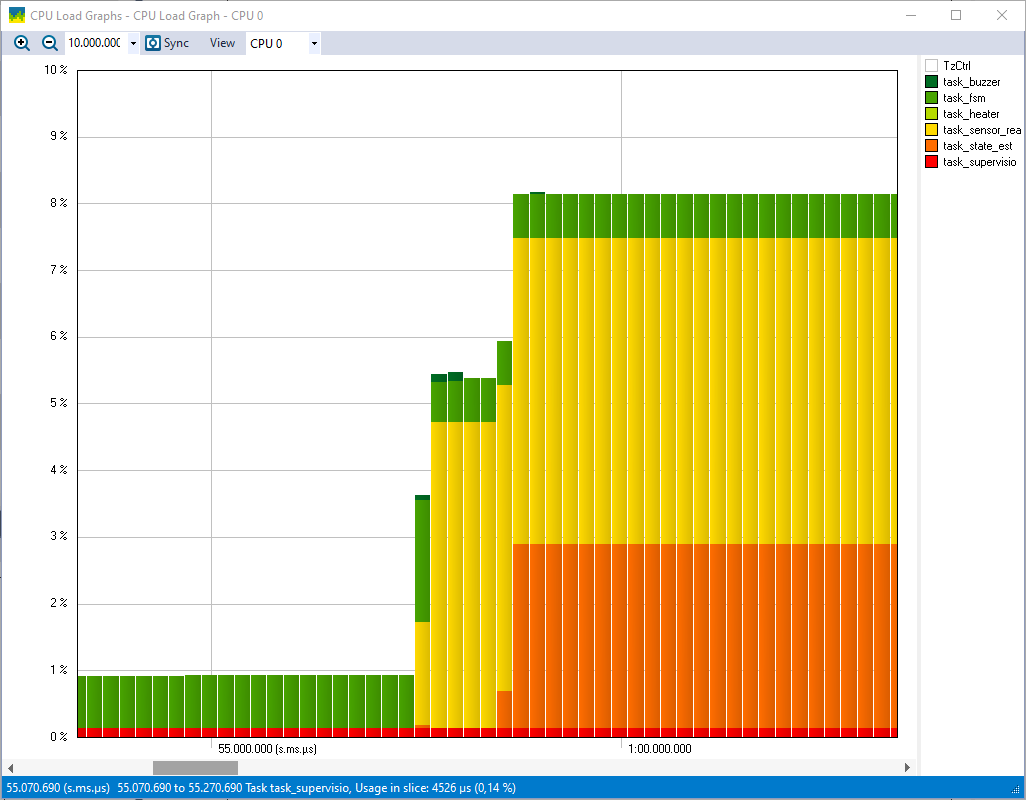
\includegraphics[width=7.8cm]{images/cpu-start}
	\caption{Dynamic starting of tasks in runtime}
	\label{fig:cpu-start}
\end{figure}

The timings were further validated by looking at the flow chart of task execution, depicted in Figure \ref{fig:cpu-flow}. Almost all time is spent just waiting for tasks to be ready for execution. The state estimation and the \acrshort{fsm} task are executed with a frequency of 100\,Hz while the sensor read task executes twice as often to read out the temperature and pressure.
\begin{figure}[h!]
    \centering
	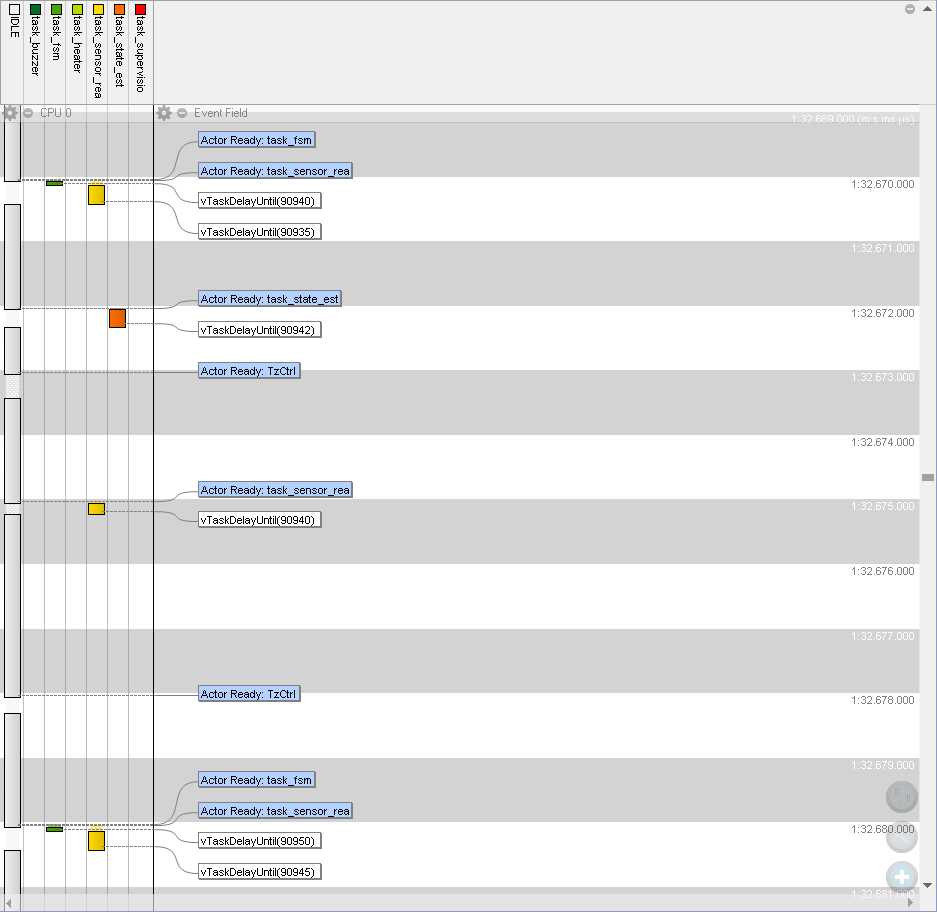
\includegraphics[width=7.8cm]{images/cpu-flow}
	\caption{Trace view of task execution}
	\label{fig:cpu-flow}
\end{figure}

Last but not least, the stack usage of all tasks was readout. The stack usage in FreeRTOS is not defined in bytes but in 32-bit integers. All tasks have more than 64 integers of stack left.


\subsubsection{Test success}
With the help of Tracealyzer, it was possible to prove that all timings and the stack usage are within an acceptable range. Furthermore, during testing, no unexpected observations were discovered.

The only part of the software that could not be analyzed with the trace is the \acrshort{cli}. Since both the trace and \acrshort{cli} share the \acrshort{usb} port, the task is disabled while tracing. Luckily this is not an issue for flight, as the \acrshort{cli} task is not running during that phase.

\newpage

\section{Drone Flight}
The purpose of the drone flight is to validate the state estimation before flying on a rocket. The test took place on the 12th of May, 2022. 

\begin{figure}[h!]
	\centering
	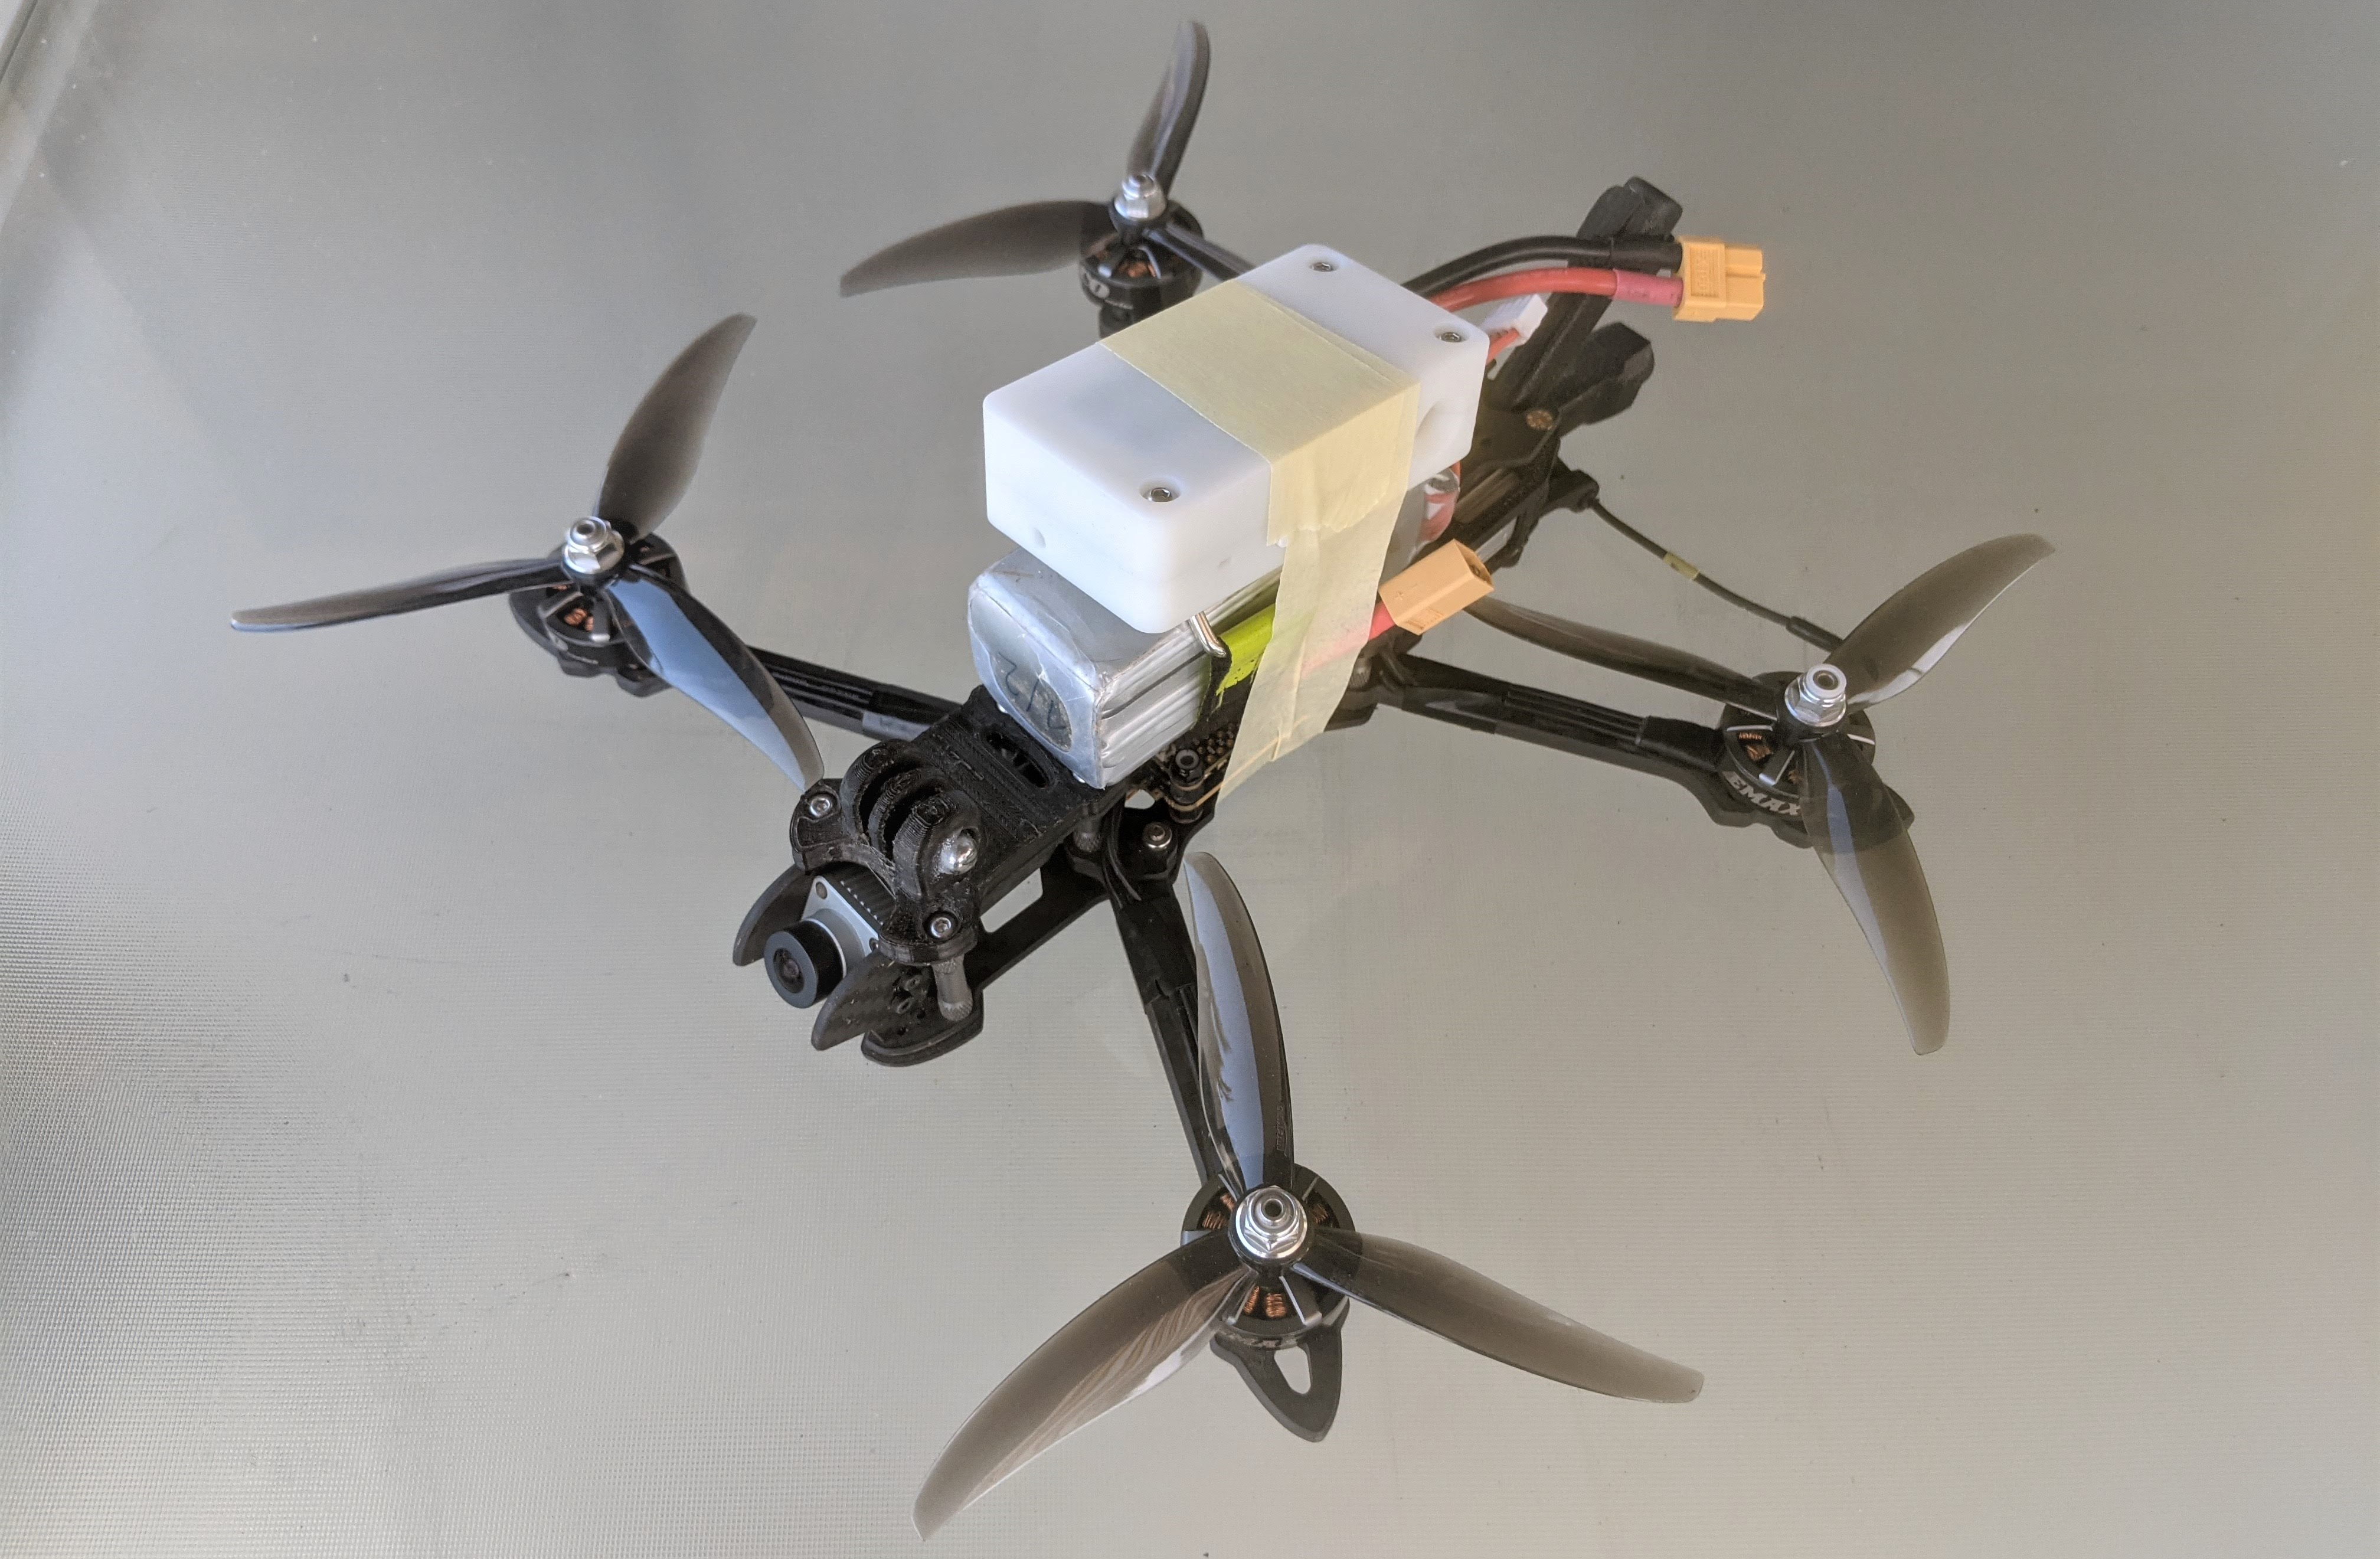
\includegraphics[width=\textwidth]{images/fpv}
	\caption{\acrshort{fpv} drone used for test flight with reefing system taped on top}
	\label{fig:fpv-drone}
\end{figure}

\subsubsection{Scope of Test}
The scope of the drone flight is to validate the state estimation. In detail, the following functions should be tested:
\begin{itemize}
    \item Liftoff detection with accelerometer
    \item Kalman Filter velocity and altitude estimation
    \item Correct state switching
    \item Data logging
\end{itemize}

\subsubsection{Acceptance criteria}
The test is successful if
\begin{itemize}
    \item All flight phases are detected
    \item The Kalman Filter estimations are realistic
    \item The data can be retrieved and analyzed after the test
\end{itemize}

\subsection{Test Setup}
The drone used for the test is a \acrshort{fpv} racing drone, built for high-speed maneuvers. With accelerations of up to 4\,g, the drone allows the simulation of a rocket flight. During this test, no reefing line was inserted to avoid stings from getting entangled in the propellers. For that reason, the burn duration was set to 5 seconds, and the main altitude was left at the default 100\,m.

In order to reproduce the flight profile of a rocket as closely as possible, the drone accelerates upward as fast as possible. At around 150\,m above ground level, the power is reduced for it to descend back to the ground.

\subsection{Results}
\subsubsection{Measurements and Observations}
The full duration of the drone flight was logged to the onboard memory. The flight logs were parsed and plotted using the jupyter notebook. The generated plots are shown in Figure \ref{fig:drone-altitude} and \ref{fig:drone-velocity}. 

\begin{figure}[h!]
	\centering
	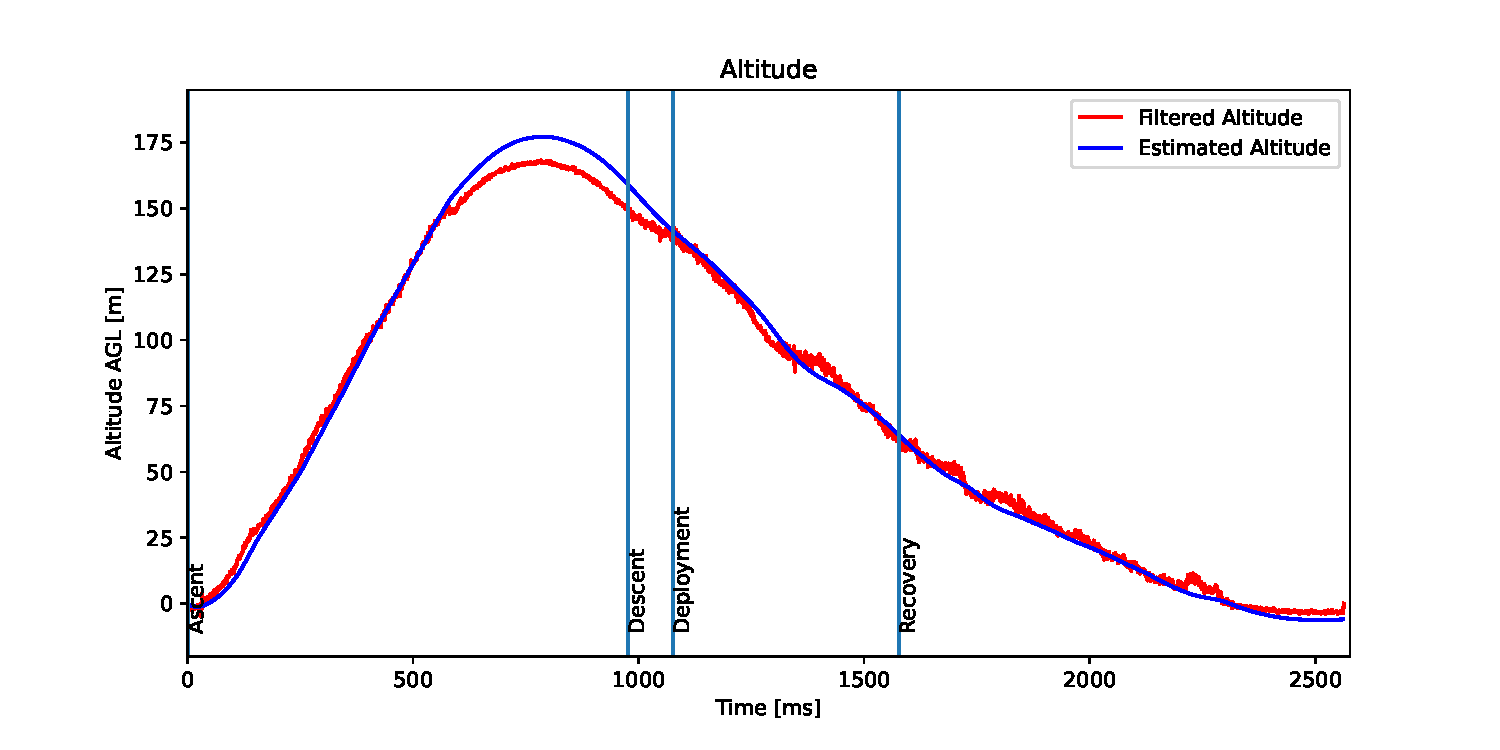
\includegraphics[width=\textwidth]{plots/drone-altitude}
	\caption{Altitude plot from flight log}
	\label{fig:drone-altitude}
\end{figure}

\begin{figure}[h!]
	\centering
	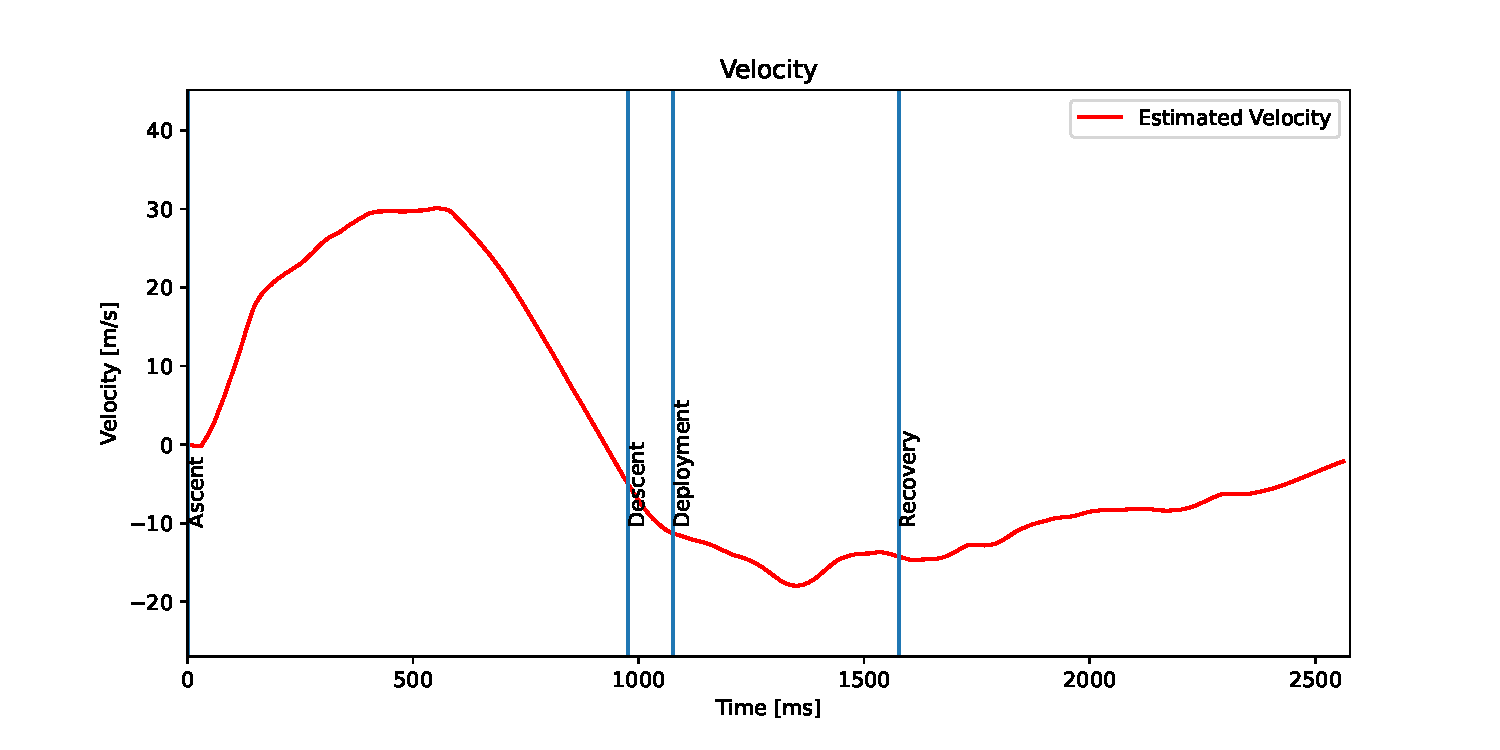
\includegraphics[width=\textwidth]{plots/drone-velocity}
	\caption{Velocity plot from flight log}
	\label{fig:drone-velocity}
\end{figure}

The filtered altitude is the moving average altitude calculated before passing it into the Kalman filter. The estimated altitude is a lot smoother than the filtered altitude. 

The filter dynamics are tuned for a rocket flight, where velocity changes are slowly reaching zero. Therefore the filter overestimated the apogee and consequently detected the descent phase late. Since the drone flight is very short, this delay is visible. However, it is of no concern, as rocket flights are a lot longer.

The velocity estimate is lagging about two seconds behind the actual velocity. As already explained in Section \ref{filter-tuning} the filter is purposely tuned to be slow but accurate. For that reason, the result is expected.

\subsubsection{Test success}
Overall, the test was successful and provided data about the state estimation performance in flight. Compared to simulations done beforehand, the actual data matches them perfectly. No unexpected observations were discovered, and the system is ready for the first rocket flight. 


\newpage

\section{Rocket Flight}
In order to fully validate the system, a full-scale rocket flight was conducted on the 14th of May, 2022. The rocket flight was in cooperation with ARGOS, a Swiss rocketry association. 

\begin{figure}[h!]
	\centering
	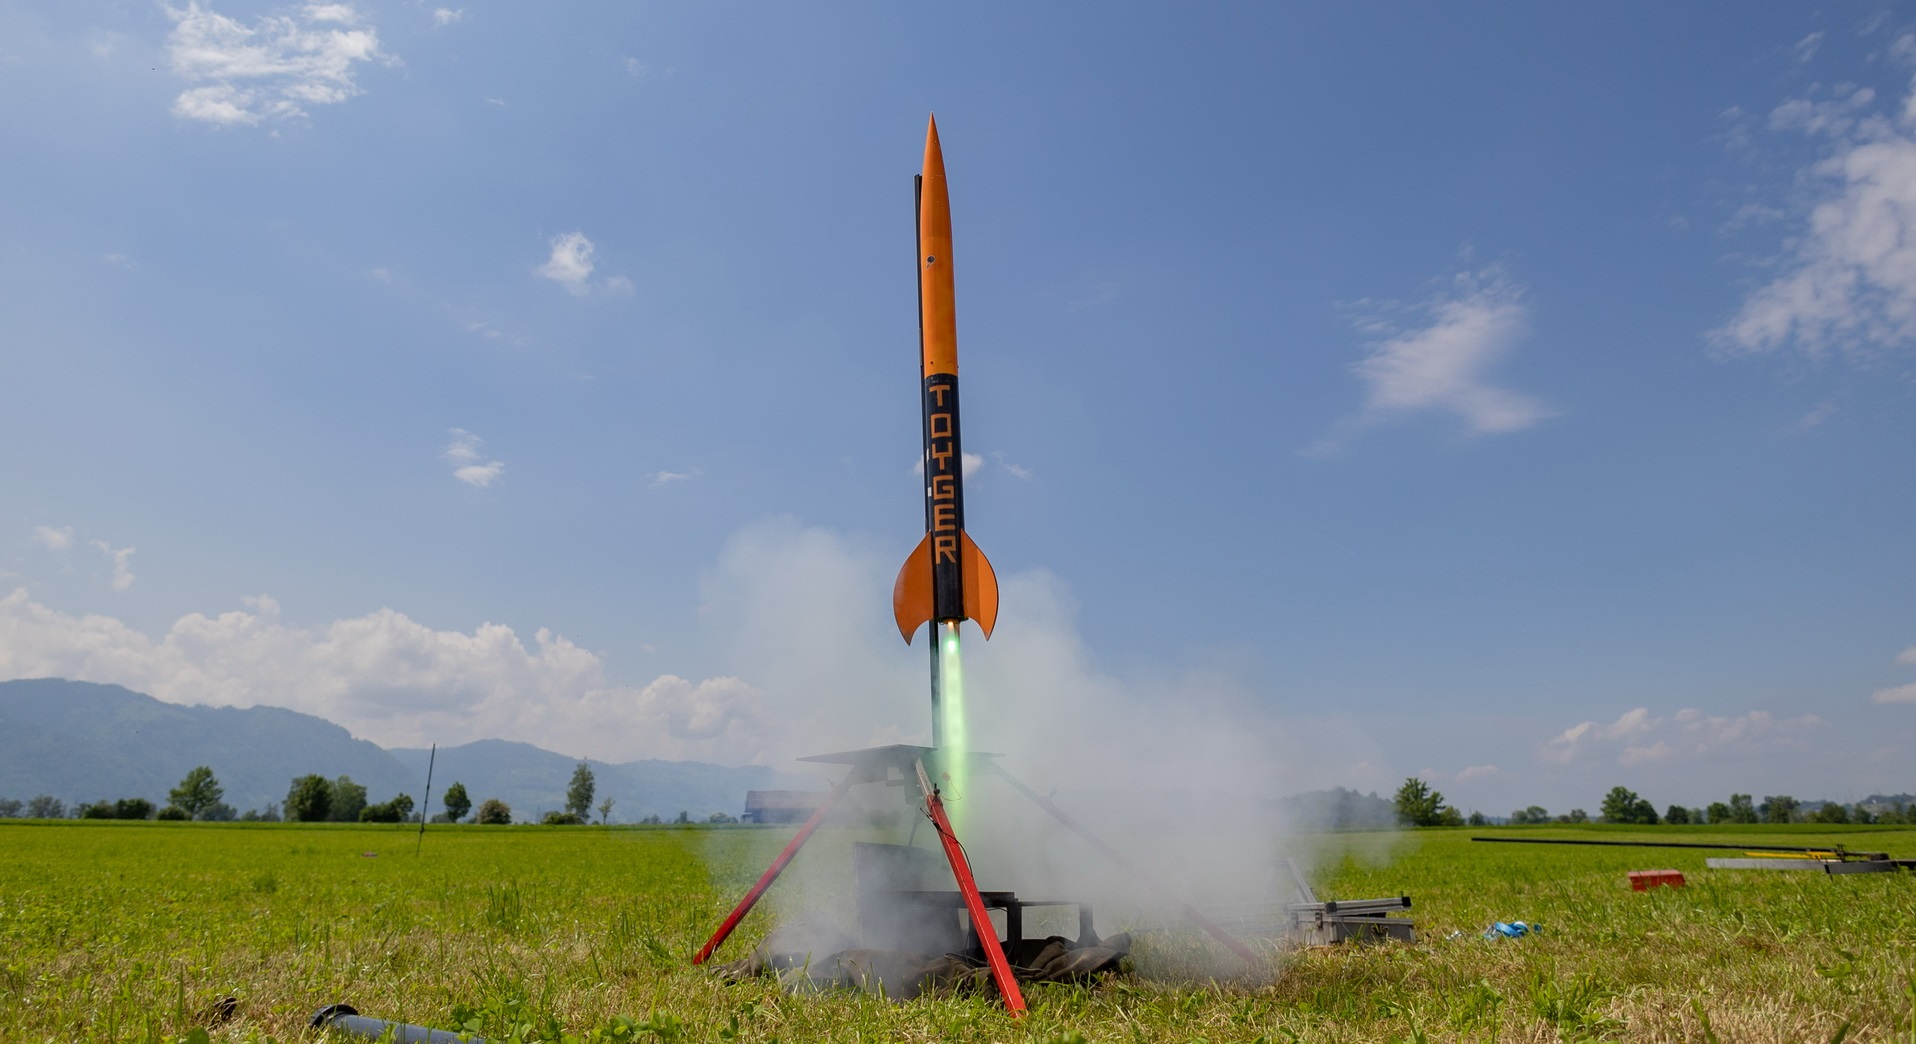
\includegraphics[width=\textwidth]{images/toyger}
	\caption{Rocket \emph{Toyger} lifting off from the launch rail in Kaltbrunn}
	\label{fig:operation}
\end{figure}

\subsubsection{Scope of Test}
The scope of the rocket flight test is to verify the operation in a real-world environment. In detail, the following functions should be tested:

\begin{itemize}
    \item Power management over an extended period
    \item Liftoff detection while the reefing computer is in sleep mode (wake up from accelerometer)
    \item Kalman Filter velocity and altitude estimation
    \item Separation of the reefing line
    \item Data logging during the flight
\end{itemize}

\subsubsection{Acceptance criteria}
The test is successful if
\begin{itemize}
    \item The reefing line gets separated during the descent of the rocket
    \item The Kalman Filter roughly estimates the altitude and velocity of the rocket
    \item The data can be retrieved and analyzed after the test
\end{itemize}

\subsection{Test Setup}
The rocket named Toyger is the rocket conducting the test. It is 178cm long and has a dry mass of almost 2kg. The rocket was constructed from a build kit and is made out of cardboard and wood. Epoxy was added to the outer walls to strengthen the material.

The rocket has flown five times before and is an excellent fit for the test as it is a proven design. 
\subsubsection{Parachute Setup}
The rocket is equipped with a single 137cm diameter parachute for recovery. A reefing ring was added to each suspension line of the parachute, and a reefing line was pulled through. In addition, the Reefing System was added to the line and securely mounted to the upper side of a canopy gore using tape. 

The parachute gets ejected at apogee by a redundant black powder charge, pushing the motor section tube and nosecone apart. The parachute is pulled out, and the descent of the flight starts. 

\subsubsection{Reefing System Configuration}
The biggest concern before the test was that the heating element does not reach the appropriate temperature in time to separate the reefing line. Because of that, the following configuration was chosen.

Preheating of the heating element is turned on from the rocket's launch. A burn duration of 30\,s was configured, forcing the computer to start heating at full power beginning at apogee. 

\subsection{Results}

\subsubsection{Measurements and Observations}
During the flight, the system was constantly logging data. After the flight, the logs were pulled from the device and plotted. The plots are shown in Figure \ref{fig:argos-altitude} and \ref{fig:argos-velocity}. 

\begin{figure}[h!]
	\centering
	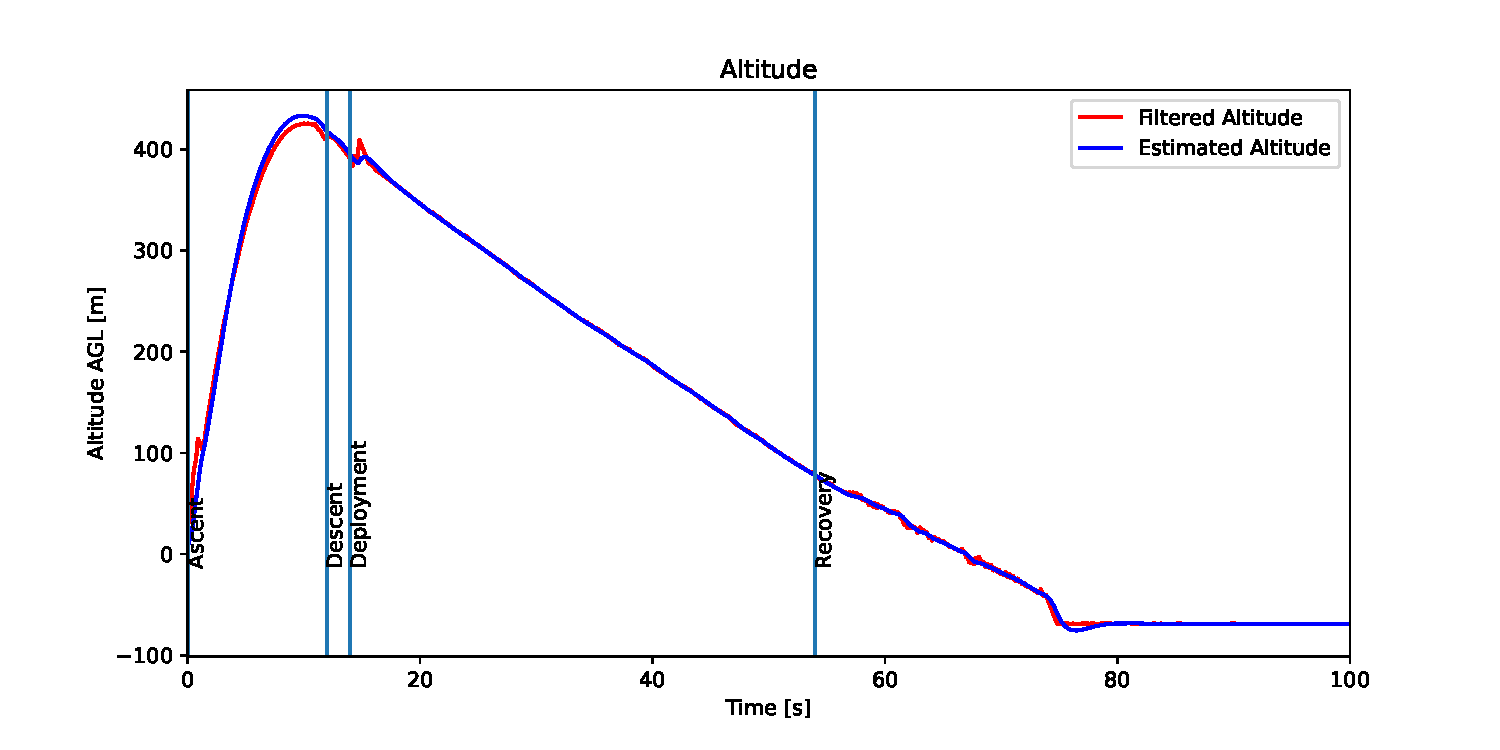
\includegraphics[width=\textwidth]{plots/argos-altitude}
	\caption{Altitude plot from flight log}
	\label{fig:argos-altitude}
\end{figure}

\begin{figure}[h!]
	\centering
	\includegraphics[width=\textwidth]{plots/argos-velocity}
	\caption{Velocity plot from flight log}
	\label{fig:argos-velocity}
\end{figure}

The state estimation worked flawlessly during all phases of the flight. One thing to note is that in Figure \ref{fig:argos-altitude} the estimated altitude did go below zero after touchdown, even though the rocket landed above its liftoff point. This occurrence can be explained by the fact that the system is sleeping before liftoff and does not adjust the zero altitude for about an hour. Temperature and pressure changes during that hour are not taken into account. This behavior was not unexpected but will need to be fixed in the future.  

After the rocket hit apogee, the parachute was ejected and immediately disreefed. Resulting in a slow descent to the ground. As shown in Figure \ref{fig:toyger-parachute} the reefing computer is still attached to the parachute, and the reefing line is cut.

\begin{figure}[h!]
	\centering
	\includegraphics[width=10cm]{images/toyger-parachute}
	\caption{Descent with disreefed parachute}
	\label{fig:toyger-parachute}
\end{figure}

\subsubsection{Test success}
The reefing computer separated the line, logged all data during the flight, and estimated the velocity and altitude to acceptable levels. Therefore the test validated some of the most critical aspects of the flight. 

\subsubsection{Unexpected Observations}
One of the black powder charges failed to ignite at apogee, forcing the rocket into a free fall for around 6 seconds after apogee. Luckily the second black powder charge fired and ejected the parachutes. The cause is most likely improper preparation of the ejection mechanism and has nothing to do with the Reefing System.

On the other hand, a problem related to the Reefing System is the early separation of the reefing line. As soon as the parachute was ejected, the line separated, advancing it to the fully open stage. The behavior observed was not easily explainable in the beginning. Unfortunately, the line was not recovered after the flight as it was not attached to the parachute. Without the line, the conclusion is open to speculation. The line ripping from the shear forces was quickly disputed, as the shear strength of the reefing line is higher than the shear strength of the suspension line, therefore making it impossible for the reefing line to rip first. It was concluded that the temperature rise of the element was a lot quicker during the flight than during ground testing. The quicker temperature increase can be explained when taking into account external factors. The rocket was fully assembled and sitting in the sun for an hour, heating the inside to over 45$^{\circ}$C. During the rocket's ascent, the system was preheating the element for about 14 seconds. Without any air circulation and being well isolated by the parachute, the temperature most likely reached the melting point of the reefing line much quicker than in testing on an open bench. As a result, the line was melted enough to separate as soon as the parachute ejected.

Another observation after the flight is that the timestamp overflowed after 65.535 seconds. The cause of that is that a 16\,bit unsigned integer is used to timestamp the data. After 65535\,ms, the integer overflows and returns to zero. This issue will not be resolved on the computer side as the increase to a 32\,bit integer would reduce the number of data points significantly. The overflow does not impact data integrity and is only fixed in the parsing stage. Whenever the timestamp decreases, $2^{16}$ is added to the rest of the data points, fixing the issue altogether.

\subsubsection{Things to improve}
Although the test was overall very successful, there are some things to improve.
\begin{itemize}
    \item The ambient temperature needs to be considered when preheating the element. A software update that enables the preheating only while below a certain threshold can be easily added.
    \item More test flights are needed to improve the timing of the separation.
    \item The reefing line should always be attached to the parachute on the opposite side of the reefing cutter. The line can help a lot in the post-flight analysis. For example, burn marks on multiple spots of the line indicate that the line was moving a lot while the element was heating.
    \item Before liftoff, the system needs to periodically wake up and reset the liftoff position to prevent altitude drifts. 
\end{itemize}

\chapter{Summary \& Conclusion}
To summarize, a fully comprehensive device has been developed. With it, parachute reefing lines can be separated during flight. A Kalman filter was designed and implemented on the hardware to estimate the velocity and altitude of the rocket. Additional software tools were created to simulate the state estimation and plot flight data. In order to change settings on the device, a user interface is presented. To protect the hardware from its surroundings, a sturdy enclosure was designed. Lastly, an extensive testing campaign was performed to assess the device's functionality.

All requirements defined in the task definition have been satisfied. The only pending aspect is the usage of the telemetry data. The implementation of this feature has been neglected because the telemetry part on the primary flight computer is not fully implemented yet. However, this functionality can easily be added in the future if necessary.

\section{Continuing Work}
Although the designed reefing system provides a rich set of features, there are some aspects to improve and add.\\
The following continuations are possible:

\begin{itemize}
		\item Testing the device on more rocket flights. The test results can help tune the system for accurate parachute disreefing. 
		\item Adding the light sensor to the software. The sensor can provide information about the deployment point of the parachute.  
		\item Support telemetry operation. The data from the rocket's main body is more accurate than the onboard data.
		\item Periodically reset the zero altitude while waiting for the rocket to lift off. This is very important to reduce the drift of altitude before a flight. 
		\item Cost reduction of the hardware. This can be achieved by removing unused parts like the thermocouple interface and ideal diode controller.
		\item Investigate more powerful heating element options to separate the reefing line quicker.
		\item Size and weight reduction by reducing battery size and case design. 
\end{itemize}

\section{Reflection \& Project Schedule}
A detailed project schedule with the planned and actual working hours can be found in Appendix \ref{fig:project_schedule}.

My time management during the project was excellent, all milestones were reached as scheduled, and all functions were implemented on time. At one point in the project cycle, I was even two weeks ahead of schedule. Some parts of the firmware turned out to be more complicated than expected, resulting in long workdays to move forward. The enclosure design was backtracked a few times to add improvements and reduce weight. Unfortunately, during the project's development phase, the report was put on hold. As a result, in the last few weeks, all my free time was spent working on the report. Overall I worked a lot more hours than initially targeted. Primarily the report required a lot more work than expected.   

\section{Personal Reflection}

In general, this thesis overall has been delightful. Within just a few weeks, I transformed an idea into a working product. The Reefing System is working as designed, and I am looking forward to seeing the device being used in large rockets. During the project, I could leverage my previous experience and build on it. I found it fascinating to learn more about all the parachute systems used in space flight and how reefing line cutters are implemented. Working with embedded systems is something I have always liked, and this project was no exception. Developing with real-time operating systems and complex logic is something I enjoy. 

I had trouble with time management in past projects, so I made sure to develop a realistic timetable this time. Spending the extra time on the schedule has proven to be very advantageous as I was able to deliver all tasks on time. 

One thing I was struggling with was the amount of text and images I needed to produce for the report. Typically these projects are done in pairs, reducing the workload on the documentation side.

Altogether I am very proud of what I achieved in such a short time frame. 


\appendix
\chapter{Appendix}
\clearpage

\section{Declaration of Authorship} \label{Declaration of Authorship}
We hereby certify that the thesis we are submitting is entirely our own original work except where otherwise indicated. I am aware of the University’s regulations concerning plagiarism, including those regulations concerning disciplinary actions that may result from plagiarism. Any use of the works of any other author, in any form, is properly acknowledged at their point of use.

\bigskip
\textbf{Location, Date} \\
Rapperswil, 03. June 2022

\vspace{1.2cm}
\begin{tabular}{@{}p{0.1cm}p{6cm}p{0.6cm}p{6cm}@{}}
& \hrulefill \\[-0.3em]
& Luca Jost\\
\end{tabular}

\includegraphics[width=4.8cm, align=t, smash=br, hshift=0.9cm, vshift=2.55cm]{appendix/Signature_Luca_Jost.pdf}

\newpage

\section{Project Schedule} \label{fig:project_schedule}
\enlargethispage{2.5cm}
\begin{adjustwidth}{0.23cm}{0cm} \hfuzz=7.0pt \vfuzz=20.0pt
\makebox[\textwidth]{\includegraphics[angle=90, width=17.3cm, page=1]{appendix/Project_Schedule_220601.pdf}}
\end{adjustwidth}
\newpage

\section{Task Definition} \label{apx:assignment}
\enlargethispage{2.5cm}
\begin{adjustwidth}{-0.23cm}{0cm} \hfuzz=7.0pt \vfuzz=20.0pt
\makebox[\textwidth]{\includegraphics[width=17.3cm, page=1]{appendix/thesis-assigment}}
\end{adjustwidth}
\newpage

\begin{adjustwidth}{-0.23cm}{0cm} \hfuzz=7.0pt \vfuzz=20.0pt
\makebox[\textwidth]{\includegraphics[width=17.3cm, page=2]{appendix/thesis-assigment}}
\end{adjustwidth}
\newpage

\begin{adjustwidth}{-0.23cm}{0cm} \hfuzz=7.0pt \vfuzz=20.0pt
\makebox[\textwidth]{\includegraphics[width=17.3cm, page=3]{appendix/thesis-assigment}}
\end{adjustwidth}
\newpage

\begin{adjustwidth}{-0.23cm}{0cm} \hfuzz=7.0pt \vfuzz=20.0pt
\makebox[\textwidth]{\includegraphics[width=17.3cm, page=4]{appendix/thesis-assigment}}
\end{adjustwidth}
\newpage

\begin{adjustwidth}{-0.23cm}{0cm} \hfuzz=7.0pt \vfuzz=20.0pt
\makebox[\textwidth]{\includegraphics[width=17.3cm, page=5]{appendix/thesis-assigment}}
\end{adjustwidth}
\newpage


\section{Kalman Filter Discretization \& Implementation}\label{apx:kalman}
\subsection{Discretization}
In order to implement the system in the real world, the filter needs to be discretized. This step is done with the zero-order hold discretization to convert the continuous-time state space system to a discrete-time model with a fixed timestep.\cite{kalman-discretization}

Applying the zero-order hold method we get
\begin{equation}
\begin{split}
    Ad & = \mathrm{e}^{AT_s} \\
    Gd & = \int_0^{T_s} \mathrm{e}^{At} G \,\mathrm{d}t \\
    Hd & = H
\end{split}
\end{equation}

Applying the Taylor series for $Ad$ we get

\begin{equation}
\begin{split}
    Ad & = \displaystyle\sum_{n=1}^{\infty} \frac{{T_s}^n A^n}{n!} \\
    & = \mathbb{I} + AT + \frac{A^2 T^2}{2!} + ...\\
    & = \begin{bmatrix}1 & 0 \\ 0 & 1 \end{bmatrix} + \begin{bmatrix}0 & T_s \\ 0 & 0 \end{bmatrix} + \begin{bmatrix}0 & 0 \\ 0 & 0 \end{bmatrix} + ... \\
    & = \begin{bmatrix}1 & T_s \\ 0 & 1 \end{bmatrix}
\end{split}
\end{equation}

By using the result from above and solving the integral we can solve $Gd$
\begin{equation}
\begin{split}
    Gd & = \int_0^{T_s} \begin{bmatrix}1 & t\\ 0 & 1 \end{bmatrix} \begin{bmatrix}0 \\ 1 \end{bmatrix} \,\mathrm{d}t \\
    & = \int_0^{T_s} \begin{bmatrix} t \\ 1 \end{bmatrix} \,\mathrm{d}t \\
    & = \begin{bmatrix} \frac{t^2}{2} \\ t \end{bmatrix} \bigg|_0^{T_s} \\
    & = \begin{bmatrix} \frac{{T_s}^2}{2} \\ {T_s} \end{bmatrix}
\end{split}
\end{equation}

\newpage

\subsection{Implementation}
The system is now fully defined and the standard Kalman Filter equations can be used.\cite{kalman-introduction}

Prediction Step
\begin{equation}
    \hat{x_k} = A \bar{x}_{k-1}
\end{equation}
where
\begin{itemize}
    \item $\hat{x}$ is the predicted state estimate;
    \item $\bar{x}_{k-1}$ is the previous updated estimate.
\end{itemize}

\begin{equation}
    \bar{P_k} = A \hat{P}_{k-1} A^T + Gd Q Gd^T
\end{equation}
where
\begin{itemize}
    \item $\bar{P_k}$ is the predicted error covariance;
    \item $Q$ is the acceleration covariance $\sigma_a$.
\end{itemize}

Update Step
\begin{equation}
    K_k = \bar{P}_k H^T(R + H \bar{P}_k H^T)^{-1}
\end{equation}
where
\begin{itemize}
    \item $K_k$ is the Kalman gain;
    \item $R$ is the altitude measurement covariance $\sigma_R$.
\end{itemize}

\begin{equation}
    \bar{x_k} = \hat{x_k} + K_k(y-H\hat{x_k})
\end{equation}
where
\begin{itemize}
    \item $\bar{x_k}$ is the updated state estimate;
    \item $y$ is the altitude measurement. 
\end{itemize}

\begin{equation}
    \hat{P_k} = (\mathrm{I} - K_k H)\bar{P}
\end{equation}
\begin{itemize}
    \item $\hat{P_k}$ is the updated error covariance.
\end{itemize}

\newpage

\section{Reefing-System Schematics} \label{apx:schematic}
\enlargethispage{2.5cm}
\begin{adjustwidth}{-0.23cm}{0cm} \hfuzz=7.0pt \vfuzz=20.0pt
\makebox[\textwidth]{\includegraphics[angle=90, width=17.3cm, page=1]{appendix/Reefing System Schematics}}
\end{adjustwidth}
\newpage

\begin{adjustwidth}{0.23cm}{0cm} \hfuzz=7.0pt \vfuzz=20.0pt
\makebox[\textwidth]{\includegraphics[angle=90, width=17.3cm, page=2]{appendix/Reefing System Schematics}}
\end{adjustwidth}
\newpage

\begin{adjustwidth}{-0.23cm}{0cm} \hfuzz=7.0pt \vfuzz=20.0pt
\makebox[\textwidth]{\includegraphics[angle=90, width=17.3cm, page=3]{appendix/Reefing System Schematics}}
\end{adjustwidth}
\newpage

\begin{adjustwidth}{-0.23cm}{0cm} \hfuzz=7.0pt \vfuzz=20.0pt
\makebox[\textwidth]{\includegraphics[angle=90, width=17.3cm, page=4]{appendix/Reefing System Schematics}}
\end{adjustwidth}
\newpage

\begin{adjustwidth}{-0.23cm}{0cm} \hfuzz=7.0pt \vfuzz=20.0pt
\makebox[\textwidth]{\includegraphics[angle=90, width=17.3cm, page=5]{appendix/Reefing System Schematics}}
\end{adjustwidth}
\newpage

\begin{adjustwidth}{-0.23cm}{0cm} \hfuzz=7.0pt \vfuzz=20.0pt
\makebox[\textwidth]{\includegraphics[angle=90, width=17.3cm, page=6]{appendix/Reefing System Schematics}}
\end{adjustwidth}
\newpage

\begin{adjustwidth}{-0.23cm}{0cm} \hfuzz=7.0pt \vfuzz=20.0pt
\makebox[\textwidth]{\includegraphics[angle=90, width=17.3cm, page=7]{appendix/Reefing System Schematics}}
\end{adjustwidth}
\newpage

\begin{adjustwidth}{-0.23cm}{0cm} \hfuzz=7.0pt \vfuzz=20.0pt
\makebox[\textwidth]{\includegraphics[angle=90, width=17.3cm, page=8]{appendix/Reefing System Schematics}}
\end{adjustwidth}
\newpage

\begin{adjustwidth}{-0.23cm}{0cm} \hfuzz=7.0pt \vfuzz=20.0pt
\makebox[\textwidth]{\includegraphics[angle=90, width=17.3cm, page=9]{appendix/Reefing System Schematics}}
\end{adjustwidth}
\newpage

\begin{adjustwidth}{-0.23cm}{0cm} \hfuzz=7.0pt \vfuzz=20.0pt
\makebox[\textwidth]{\includegraphics[angle=90, width=17.3cm, page=10]{appendix/Reefing System Schematics}}
\end{adjustwidth}
\newpage

\begin{adjustwidth}{-0.23cm}{0cm} \hfuzz=7.0pt \vfuzz=20.0pt
\makebox[\textwidth]{\includegraphics[angle=90, width=17.3cm, page=11]{appendix/Reefing System Schematics}}
\end{adjustwidth}
\newpage

\begin{adjustwidth}{-0.23cm}{0cm} \hfuzz=7.0pt \vfuzz=20.0pt
\makebox[\textwidth]{\includegraphics[angle=90, width=17.3cm, page=12]{appendix/Reefing System Schematics}}
\end{adjustwidth}
\newpage

\begin{adjustwidth}{-0.23cm}{0cm} \hfuzz=7.0pt \vfuzz=20.0pt
\makebox[\textwidth]{\includegraphics[angle=90, width=17.3cm, page=13]{appendix/Reefing System Schematics}}
\end{adjustwidth}
\newpage

\section{Reefing-System Mechanical Drawing} \label{Reefing System Enclosure Mechanical Drawing}
\enlargethispage{2.5cm}
\begin{adjustwidth}{0.23cm}{0cm} \hfuzz=7.0pt \vfuzz=20.0pt
\makebox[\textwidth]{\includegraphics[angle=90, width=17.3cm, page=1]{appendix/Reefing System Mechanical}}
\end{adjustwidth}
\newpage

\section{Data Archive} \label{Data Archive}
All created files and documents of this project are publicly available on GitHub. An institution called \textbf{BA-OST-22} (\url{https://github.com/BA-OST-22}) has been created which contains repositories for each individual part of the project.
A quick description of the repositories including the associated web link is listed below:

\subsubsection{reefing-system-admin} \label{reefing-system-admin} \vspace{-0.2cm}
\begin{description}
  \item[Description:] This repository contains all confidential information of the project.\vspace{-0.25cm}
  \item[URL:] \url{https://github.com/BA-OST-22/reefing-system-admin}\vspace{-0.25cm}
  \item[Type:] Private\vspace{-0.25cm}
\end{description}

\subsubsection{reefing-system-docs} \vspace{-0.2cm}
\begin{description}
  \item[Description:] This repository contains all additional documentation of the project.\vspace{-0.25cm}
  \item[URL:] \url{https://github.com/BA-OST-22/reefing-system-docs}\vspace{-0.25cm}
  \item[Type:] Public\vspace{-0.25cm}
\end{description}

\subsubsection{reefing-system-hardware} \vspace{-0.2cm}
\begin{description}
  \item[Description:] This repository contains hardware and mechanical related documents.\vspace{-0.25cm}
  \item[URL:] \url{https://github.com/BA-OST-22/reefing-system-hardware}\vspace{-0.25cm}
  \item[Type:] Public\vspace{-0.25cm}
\end{description}

\subsubsection{reefing-system-firmware} \vspace{-0.2cm}
\begin{description}
  \item[Description:] This repository contains firmware source code written in C.\vspace{-0.25cm}
  \item[URL:] \url{https://github.com/BA-OST-22/reefing-system-firmware}\vspace{-0.25cm}
  \item[Type:] Public\vspace{-0.25cm}
\end{description}

\subsubsection{reefing-system-utilities} \vspace{-0.2cm}
\begin{description}
  \item[Description:] This repository contains all utilities for simulation, flight parsing and data plotting written in Python.\vspace{-0.25cm}
  \item[URL:] \url{https://github.com/BA-OST-22/reefing-system-utilities}\vspace{-0.25cm}
  \item[Type:] Public\vspace{-0.25cm}
\end{description}

\backmatter

\bibliographystyle{plain}
\typeout{}
\bibliography{./sections/bibliography.bib}

\end{document}